\documentclass[a4paper,11pt]{article}
\pdfoutput=1 

\usepackage{jinstpub} 
\usepackage[utf8]{inputenc}
\usepackage{lineno}

\usepackage[capitalise,noabbrev,nameinlink]{cleveref}
\newlength{\abc}
\settowidth{\abc}{\space}
\AtBeginDocument{%
\renewcommand{\ref}[1]{\mbox{\Cref{#1}}}
\renewcommand{\equationautorefname}{Equation~\hspace{-\abc}}
\renewcommand{\sectionautorefname}{Section\,\negthinspace}
\renewcommand{\subsectionautorefname}{Section\,\negthinspace}
\renewcommand{\subsubsectionautorefname}{Section\,\negthinspace}
\renewcommand{\figureautorefname}{Figure\,\negthinspace}
\renewcommand{\tableautorefname}{Table\,\negthinspace}
}

% si units
\usepackage[binary-units=true]{siunitx}

% multirows in tables
\usepackage{multirow}

\usepackage{textcomp}
\usepackage{xcolor}
\usepackage{graphicx}
\usepackage{mathtools}
\usepackage{subcaption}
\usepackage[LGRgreek]{mathastext}
\usepackage{xspace}
%
% text handling
%

% vertical offset shortcut for paragraphs
\newcommand{\pg}[0]{\vspace*{0.75em}\newline}

% indentation shortcut
\newcommand{\ind}[0]{\hspace*{\customindent}}

% combination of vertical offset and indentation
\newcommand{\parag}{\parag\ind}


%
% content shorthands
%

% text and name highlights
\newcommand{\thl}[1]{``#1''}
\newcommand{\nhl}[1]{\textsc{#1}}

% missing citations
\newcommand{\tocite}[1]{\textbf{\textcolor{red}{[\ifthenelse{\equal{#1}{}}{?}{#1}]}}}

% arXiv and cds link
\newcommand{\arxivlink}[2]{\href{https://arxiv.org/abs/#1}{\texttt{arXiv:#1\,[#2]}}}
\newcommand{\cdslink}[1]{\href{http://cds.cern.ch/record/#1}{\texttt{cds:#1}}}

% argmin/max operators
\DeclareMathOperator*{\argmin}{arg\ min}
\DeclareMathOperator*{\argmax}{arg\ max}

% uneven plus-minus value
\newcommand{\upm}[4]{#1#2/\!#3\!#4}

%special signs
\newcommand{\inches}{\ensuremath{{}^{\prime\prime}}}
\newcommand{\skiroc}{SKIROC2-CMS}
\newcommand{\percent}{$\%$}
\newcommand{\permille}{\ensuremath{{}^\text{o}\mkern-5mu/\mkern-3mu_\text{oo}}}
\newcommand{\med}{\text{med}}

%% Units
\newcommand{\degrees}{\ensuremath{^{\circ}}\xspace}
\newcommand{\hitspermmbx}{\ensuremath{\text{Hits/mm}^{2}\text{/BX}}\xspace}
\newcommand{\permmbx}{\ensuremath{\text{/mm}^{2}\text{/BX}}\xspace}
\newcommand{\flux}{\ensuremath{\text{n_{eq}}/\text{cm}^{2}/\text{yr}}\xspace}
\newcommand{\neqcm}{\ensuremath{\mathrm{n_{eq}}/\mathrm{cm}^{2}}\xspace}
\newcommand{\percms}{\ensuremath{\text{cm}^{-2}\mathrm{s}^{-1}}\xspace}
\newcommand{\micron}{\ensuremath{\upmu\mathrm{m}}\xspace}
\newcommand{\microsecond}{\ensuremath{\upmu\mathrm{s}}\xspace}
\newcommand{\microwatt}{\ensuremath{\upmu\mathrm{W}}\xspace}

%abbreviations
\newcommand{\eg}{e.g.}
\newcommand{\ie}{i.e.}

%software
\newcommand{\CMSSW}{\textsc{CMSSW}}
\newcommand{\ROOT}{\textsc{ROOT}}
\newcommand{\corryvreckan}{\textsc{CORRYVRECKAN}}
\newcommand{\Geant}{\textsc{GEANT4}}
\newcommand{\luigi}{\textsc{LUIGI}}
\newcommand{\millepede}{\textsc{MILLEPEDE}}

%
% physics processes
%

\newcommand{\slep}{\text{single-lepton}}
\newcommand{\dlep}{\text{dilepton}}
\newcommand{\fullh}{\text{full-hadron}}
\newcommand{\Slep}{\text{Single-lepton}}
\newcommand{\Dlep}{\text{Dilepton}}
\newcommand{\Fullh}{\text{Full-hadron}}
\newcommand{\slepe}{\text{single-electron}}
\newcommand{\slepmu}{\text{single-muon}}
\newcommand{\Slepe}{\text{Single-electron}}
\newcommand{\Slepmu}{\text{Single-muon}}

\newcommand{\hf}{\text{heavy-flavor}}
\newcommand{\ttbar}{\ensuremath{t\bar{t}}}
\newcommand{\bbbar}{\ensuremath{b\bar{b}}}
\newcommand{\ccbar}{\ensuremath{c\bar{c}}}
\newcommand{\totbar}{\ensuremath{t\hspace{-0.5mm}/\hspace{-0.5mm}\bar{t}}}
\newcommand{\bobbar}{\ensuremath{b\hspace{-0.5mm}/\hspace{-0.5mm}\bar{b}}}
\newcommand{\ttH}{\ensuremath{\ttbar H}}
\newcommand{\Hbb}{\ensuremath{H\rightarrow \bbbar}}
\newcommand{\Hnbb}{\ensuremath{H\nrightarrow \bbbar}}
\newcommand{\HWW}{\ensuremath{H\rightarrow W^+W^-}}
\newcommand{\Htautau}{\ensuremath{H\rightarrow \tau^+\tau^-}}
\newcommand{\ttHbb}{\ensuremath{\ttH\,(\Hbb)}}
\newcommand{\ttHnbb}{\ensuremath{\ttH\,(\Hnbb)}}
\newcommand{\ttX}{\ensuremath{\ttbar\!+\!\text{X}}}
\newcommand{\ttbb}{\ensuremath{\ttbar\!+\!\bbbar}}
\newcommand{\ttb}{\ensuremath{\ttbar\!+\!\bobbar}}
\newcommand{\tttb}{\ensuremath{\ttbar\!+\!2b}}
\newcommand{\ttcc}{\ensuremath{\ttbar\!+\!\ccbar}}
\newcommand{\ttlf}{\ensuremath{\ttbar\!+\!\text{lf}}}
\newcommand{\tthf}{\ensuremath{\ttbar\!+\!\text{hf}}}
\newcommand{\Singlet}{\ensuremath{\text{Single}\ \totbar}}
\newcommand{\singlet}{\ensuremath{\text{single}\ \totbar}}
\newcommand{\Singlett}{\ensuremath{\text{Single}\ t}}
\newcommand{\Singletbar}{\ensuremath{\text{Single}\ \bar{t}}}
\newcommand{\Vjets}{\ensuremath{V\hspace{-0.5mm}\!+\!\text{jets}}}
\newcommand{\Wjets}{\ensuremath{W\hspace{-0.5mm}\!+\!\text{jets}}}
\newcommand{\Zjets}{\ensuremath{Z\hspace{-0.5mm}\!+\!\text{jets}}}
\newcommand{\Diboson}{\ensuremath{\text{Diboson}}}
\newcommand{\diboson}{\ensuremath{\text{diboson}}}
\newcommand{\ttW}{\ensuremath{\ttbar\!+\!W}}
\newcommand{\ttZ}{\ensuremath{\ttbar\!+\!Z}}
\newcommand{\ttV}{\ensuremath{\ttbar\!+\!V}}


%
% physics process colors
%

\definecolor{ttHcol}{RGB}{67,118,201}
\definecolor{ttbbcol}{RGB}{235,230,10}
\definecolor{ttbcol}{RGB}{205,0,10}
\definecolor{tttbcol}{RGB}{255,153,1}
\definecolor{ttcccol}{RGB}{131,38,10}
\definecolor{ttlfcol}{RGB}{81,142,25}
\definecolor{Singletcol}{RGB}{0,204,204}
\definecolor{Vjetscol}{RGB}{104,140,140}
\definecolor{Dibosoncol}{RGB}{1,25,147}
\definecolor{ttVcol}{RGB}{255,102,101}


%
% other physics variables
%

\newcommand{\BR}{\ensuremath{B\!R}}
\newcommand{\met}{\ensuremath{\cancel{E}_T}}
\DeclareRobustCommand{\orderof}{\ensuremath{\mathcal{O}}}


\title{\boldmath Neutron Irradiation and Electrical Characterisation of \\8'' Silicon Pad Sensor Prototypes for the CMS Endcap Calorimeter Upgrade}


\author[a]{Nick Hinton}
\author[b]{Timo Peltola}
\author[c]{Thorben Quast}
\author[c]{Eva Sicking}

\affiliation[a]{Brown University}
\affiliation[b]{Texas Tech University}
\affiliation[c]{CERN Experimental Physics Department}

\collaboration[d]{on behalf of the CMS HGCAL silicon group}

\emailAdd{thorben.quast@cern.ch}

\abstract{
    As part of its HL-LHC upgrade program, the CMS collaboration is planning to replace its existing endcap calorimeters with a high-granularity calorimeter (HGCAL). 
    The new calorimeter will be a sampling calorimeter with unprecedented transverse and longitudinal readout for both electromagnetic and hadronic compartments. 
    Due to its compactness, intrinsic time resolution and radiation hardness, silicon has been chosen as active material for the regions exposed to higher radiation levels. 
    The silicon sensors will be fabricated as \SI{20}{\centi\metre} (8'') wide hexagonal wafers and will be segmented into several hundred sensitive pads which will be read out individually. 
    As part of the sensor qualification strategy, sensor irradiation with neutrons at the Rhode Island Nuclear Science Center have been conducted for the first time followed by their electrical characterisation in 2020/21.
    The completion of this important milestone in the R$\&$D program for this ambitious calorimeter is documented in this work.
    This paper provides detailed account of the associated infrastructural aspects, and explains the procedures followed.
    With it, this work may serve as an instructive inspiration for future R$\&$D on the radiation hardness of large silicon structures for potential future silicon-based detector concepts.
    Last but not least, the results on the electrical properties of the irradiated HGCAL silicon sensors are presented which may serve as a practical reference for the expected degradation of HGCAL silicon sensors towards the end of its lifetime.
} 
\keywords{Calorimeter, CMS, HGCAL, silicon sensors, neutron irradiation, HL-LHC, electrical properties, leakage, dark current, depletion voltage}

\linenumbers

\begin{document}
\maketitle
\flushbottom

\linenumbers
\section{Introduction}
\label{sec:introduction}

The Large Hadron Collider at CERN will be upgraded to provide more instantaneous luminosity~\cite{hllhc-tdr:2017}.
Experiments, such as CMS, need to upgrade their detector systems. 
One of the CMS upgrades is the replacement of the current endcap calorimeters with the High Granularity Calorimeter (HGCAL)~\cite{hgcal-tdr:2018}.
Silicon sensors will be used and their electrical properties are important to assess after irradiation.
This is what we will show here.
\section{Silicon Pad Sensor Prototypes for the CMS Endcap Calorimeter Upgrade}
\label{sec:sensors}

The CMS high granularity calorimeter will be made of more than \SI{600}{\metre\squared} of planar DC-coupled silicon pad sensors.
The sensors are fabricated as 8'' hexagonal wafers.
A hexagonal sensor geometry allows for an optimal use of the circular wafer as which the silicon crystals are grown.
Motivated by empiric evidence of superior noise performance with respect to n-type sensors~\cite{Adam_2017}, p-type doping of their bulk was chosen.\newline
In this work, hexagonal wafer prototype sensors of the so-called low-density (LD) and high-density (HD) designs were irradiated with neutrons and electrically qualified.
Their design is illustrated in~\ref{fig:Sensors}.
Each HGCAL silicon sensor is segmented into several hundred pads that constitute the sensitive units. 
The majority of those pads are shaped as regular hexagons which are drawn as cyan-colored pads in~\ref{fig:Sensors}.
Special non-hexagonal structures fill out the wafer periphery.
The arrangement of pads on a wafer is enclosed and protected from external disturbance by a guard ring.
\begin{figure}
	\captionsetup[subfigure]{aboveskip=-1pt,belowskip=-1pt}
	\centering
	\begin{subfigure}[b]{0.50\textwidth}
		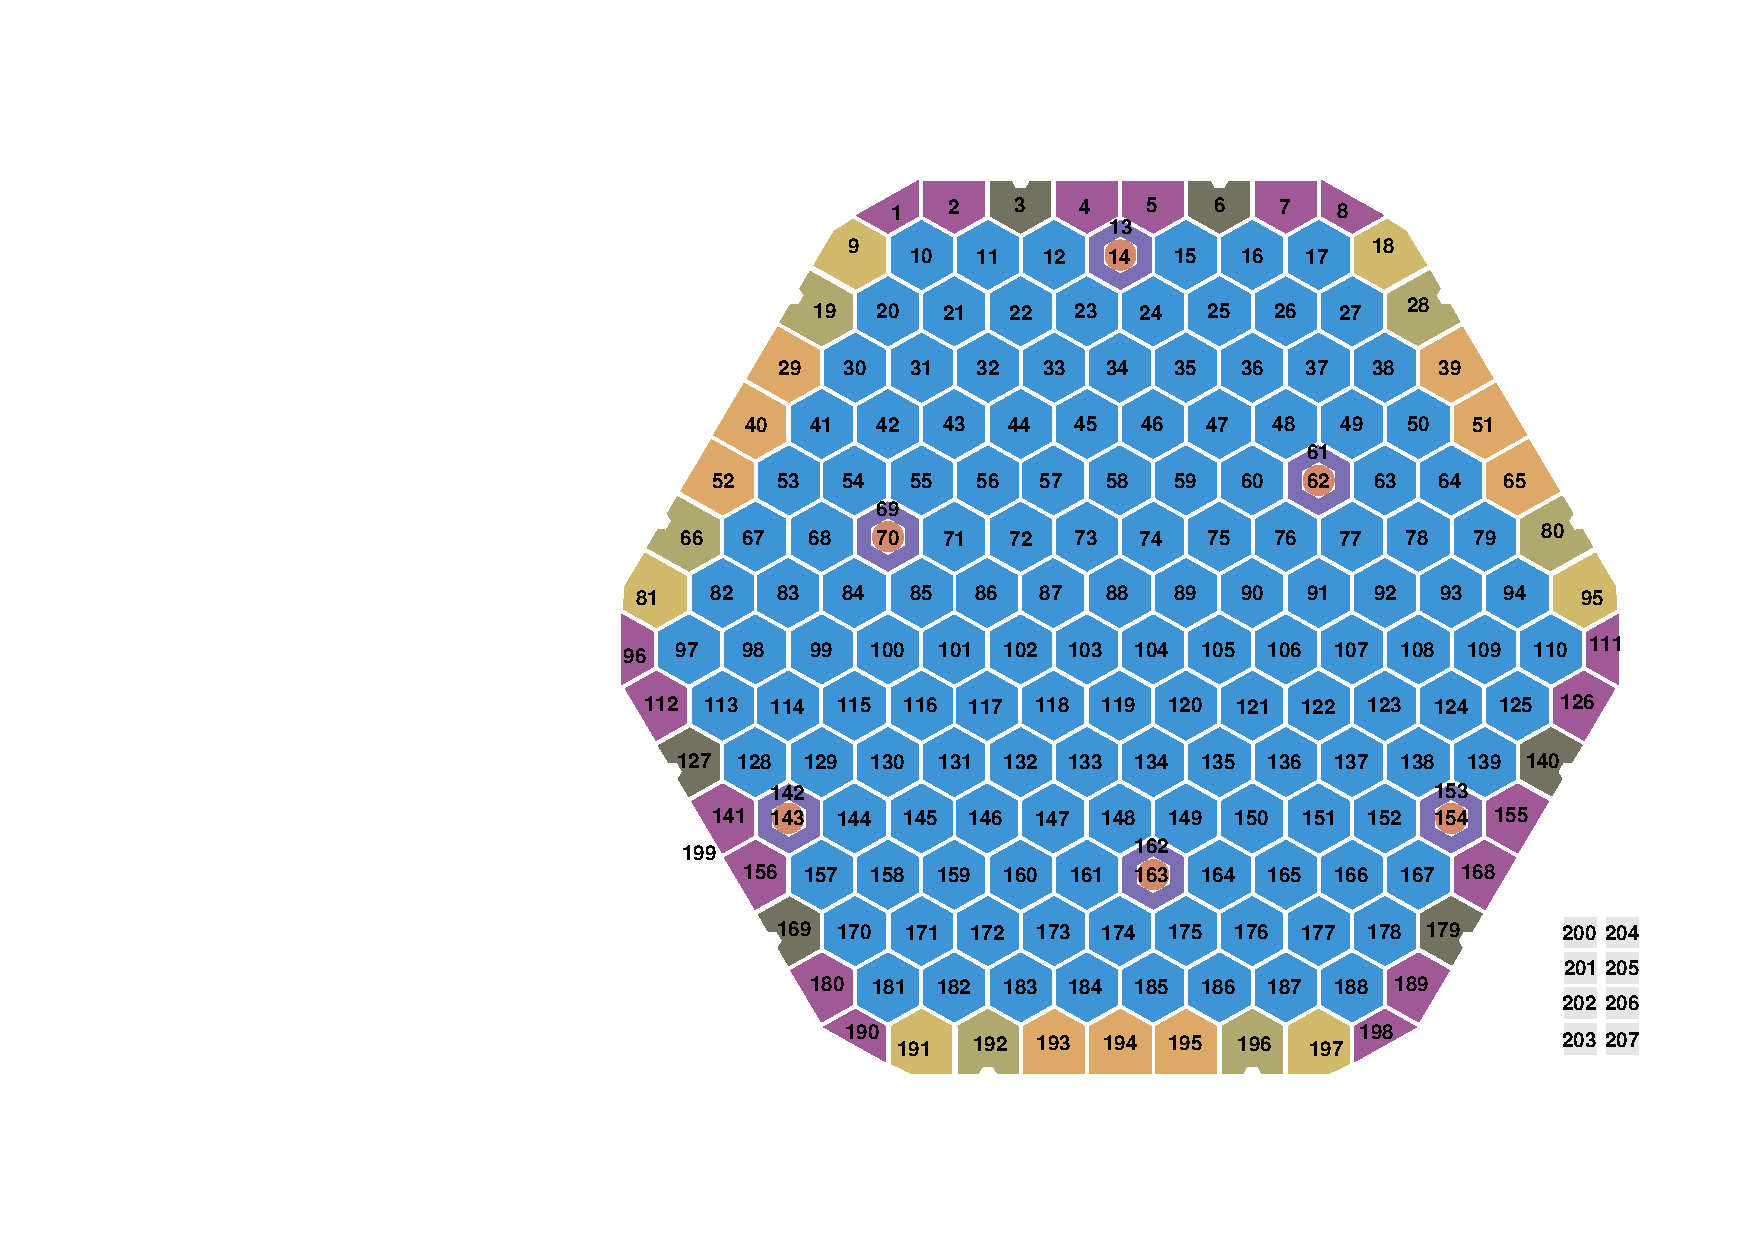
\includegraphics[width=0.999\textwidth]{plots/ch_mapping/LD.pdf}
		\subcaption{
		}
	\end{subfigure}
	\hfill
	\begin{subfigure}[b]{0.48\textwidth}
		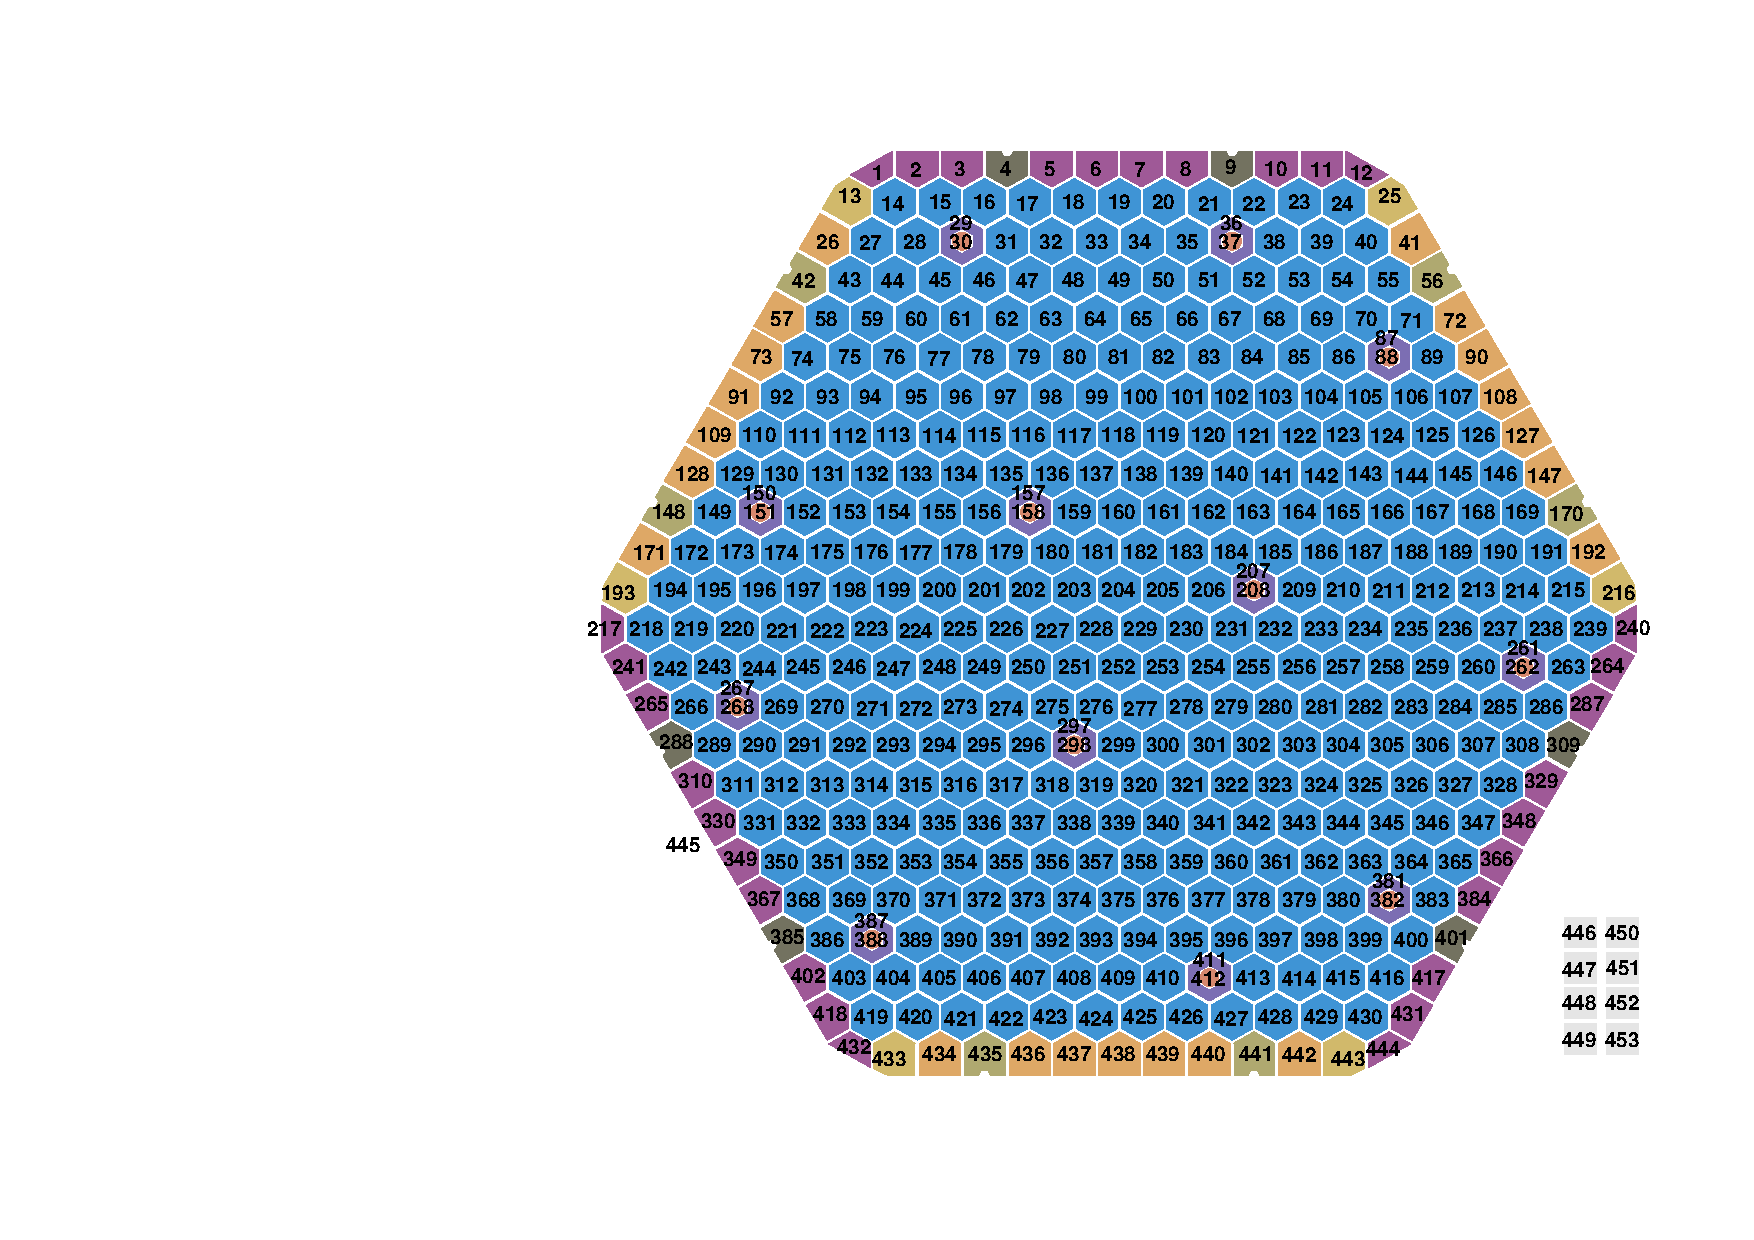
\includegraphics[width=0.999\textwidth]{plots/ch_mapping/HD.pdf}
		\subcaption{
		}
	\end{subfigure}    
	\caption{
        (a) Layout of the tested 8'' prototype silicon pad sensors with the low-density (LD) and (b) the high-density (HD) design.
		Regular hexagonal pads are depicted in cyan. 
		Small and large edge pads populate the wafer periphery. 
		Six (LD), respectively twelve (HD), regular, small hexagonal pads on the wafer are dedicated for calibration of the energy.
		The sensors guard rings are not shown.
	}
	\label{fig:Sensors}
\end{figure}
The LD sensors were produced from physically thinned p-type float zone silicon wafers.
They are segmented into 198 pads, where full hexagonal pads are about \SI{1.2}{\centi\metre\squared} large, and have an active thickness of \SI{200}{\micro\meter} or \SI{300}{\micro\meter}.
%It was found empirically~\cite{hgcal-tdr:2018} that the relative signal degradation is worse the thicker the active area of the silicon sensor is.
LD sensors will be installed in regions of intermediate radiation fluences inside HGCAL.
By contrast, regions with the highest fluences will be populated with HD sensors whose active thickness amounts to \SI{120}{\micro\meter} \footnote{Although their active thickness amounts to only \SI{120}{\micro\meter}, the physical thickness of HD sensors is \SI{300}{\micro\meter}.}.\newline
HD sensors are segmented into 444 pads (full hexagon pad size: \SI{0.5}{\centi\metre\squared}) and are produced from epitaxial on a handle wafers.
As it is foreseen for the final design, p-stop structures were added to all the tested prototype silicon sensors in this work in order to limit the accumulation of electrons between the sensitive pads.
Those structures were either bound to the single pads (individual p-stop) or shared between neighboring ones (common p-stop)~\cite{Brondolin_2020}.
In addition, the tested prototype sensors differed in their flatband voltage (either \SI{-2}{\volt} or \SI{-5}{\volt}).
Other than that, all production parameters, such as doping concentrations and the composition of the oxide layer, were identical for all prototype sensors discussed in this work.
It is noted that differences in the bulk properties are not expected to affect the sensor degradation due to irradiation~\cite{MOLL199987} and are thus not subject of this work.
\newline
Prior to irradiation, the studied sensors had been electrically qualified demonstrating their proper functionality:
Full depletion was achieved at bias voltages betweem \SI{40}{\volt} ($\pm\SI{5}{\volt}$) for \SI{120}{\micro\metre} sensors and \SI{280}{\volt} ($\pm\SI{10}{\volt}$) for \SI{300}{\micro\meter} sensors. 
Moreover, per-pad leakage currents of the non-irradiated sensors did not exceed a few nanoamperes, and the total currents at room temperatures between 20-\SI{24}{\celsius} over the full wafer remained well below \SI{100}{\micro\ampere} over the relevant range of bias voltages up to \SI{-850}{\volt}. \newline
In general, exposure of silicon sensors to radiation adds impurities to the silicon lattice which affects both the leakage currents and the depletion voltages. 
While the bulk-dominated leakage current density increases proportionally with the fluence, the expected increase of the depletion voltage (for p-type sensors) is non-trivial and its quantification beyond the scope of this work.
The interested reader is encouraged to consult Refs.~\cite{moll:SiDamages,LINDSTROM200330} for this purpose.
\section{Irradiation at the Rhode Island Nuclear Science Center}
\label{sec:irradiation}

\subsection{Rhode Island Nuclear Reactor}
\label{subsec:RINSC}
The Rhode Island Nuclear Science Center (RINSC) houses a \SI{2}{\mega\watt}, light-water cooled, pool-type reactor in Narragansett, Rhode Island, USA.
Its core consists of fuel assemblies reflected with a combination of graphite and beryllium.
The fuel is plate type U$_3$Si$_2$ cladded with aluminum enriched to less than 20$~\%$ Uranium-235.
In general, there are six different methods to irradiate materials at RINSC.
However, only the delivery method via the beamport was applicable because it is the only sample delivery system large enough to accept full-sized HGCAL silicon sensor wafers.
The beamport has not been used for the last 30 years prior to this activity.
A sketch of the beamport and a photo of its inside are shown in \ref{fig:Beamport_Schematic}a and b.
\begin{figure}[!hbt]
  \begin{center}
    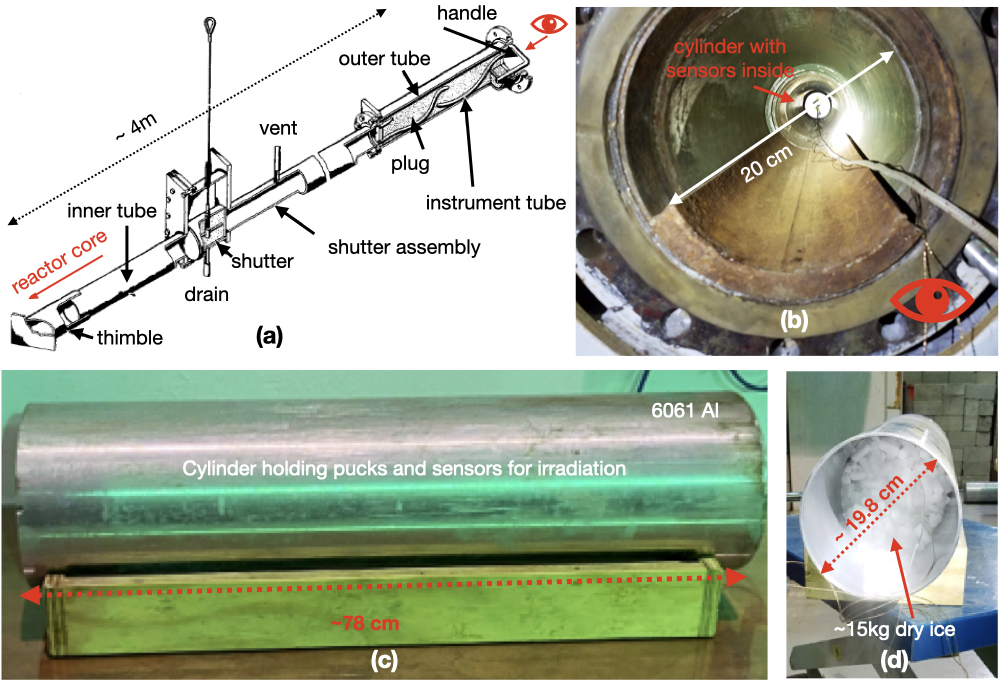
\includegraphics[width=0.99\textwidth]{figures/figures_edited_001.jpeg}
    \caption{(a) Schematic of the beamport sample delivery system at RINSC.
    (b) The view down into the beamport used for these irradiation studies.
    (c) The sample delivery cylinder that contains the sensor-holding hockey pucks and (d) dry ice for cooling of the silicon sensors in the beamport during and after irradiation.
    }
    \label{fig:Beamport_Schematic}
  \end{center}
\end{figure}
It measures about \SI{4}{\metre} from its opening to the termination near to the reactor core, and it can accommodate samples with diameters of up to \SI{20}{\centi\metre} and with depths up to \SI{90}{\centi\metre}.
A shutter assembly sits \SI{3}{\metre} from the opening of the beamport, which must be raised to allow for the insertion of the samples and closed prior to the start of the reactor.
A \SI{85}{\centi\metre}-long lead plug serves as a radiation shield that has to be inserted into the opening of the beamport prior to the start of the irradiation.

\subsection{Irradiation of HGCAL silicon sensor prototypes}
\label{subsec:irradiation}
Given the constraints of the beamport system at RINSC, a dedicated sample delivery method had to be developed for irradiation HGCAL silicon wafers.
This new sample delivery allows for:
\begin{itemize}
  \item Positioning sensors as close to the reactor core as possible,
  \item protecting them from physical damage during the loading, irradiation, and unloading,
  \item keeping the irradiated sensors at cold temperatures during the after the irradiation,
  \item and monitoring the temperature of the samples inside the breamport.
\end{itemize}
Two compatible pieces of hardware were manufactured for the irradiation of the HGCAL silicon sensor prototypes: a sensor container, referred to as a "hockey puck", and a sample delivery cylinder (see~\ref{fig:Beamport_Schematic}c). 
The former is used to protect, orient, and store the sensors during irradiation while the latter is used to protect and locate the hockey puck inside the beamport.\newline
The cylinder is made from 6061 aluminum, has an outer diameter of \SI{19.8}{\centi\metre} fitting into the beamport, and the inner diameter of the cylinder is \SI{19.1}{\centi\metre} allowing for smooth insertion and removal of the hockey pucks.
The cylinder has a welded cap on the end that faces the reactor core, and a removable cap with threaded holes for 8 to 32 countersunk flat head machine screws that are flush with the outer wall of the cylinder. 
Both the welded cap and the removable cap have vent holes to allow for air to flow into and out of the cylinder.
An eye bolt is screwed into the removable cap to facilitate removing the cylinder from the beamport after irradiations.\newline
We experimented with three different hockey puck materials, see~\ref{fig:Pucks_Arrayed}a: Oak, acrylic, and PEEK. 
Those differ in their mechanical deformation with respect to temperature fluctuations, in their activations, radiation hardness and overall cost.
As practical compromise between thse factors, we found acrylic most suitable for irradiation up to fluences of $2\cdot 10^{15}\neq$, andPEEK material suitable for higher fluences. 
\textcolor{red}{One-two sentences on the material choice.}\newline
\begin{figure}[!hbt]
  \begin{center}
    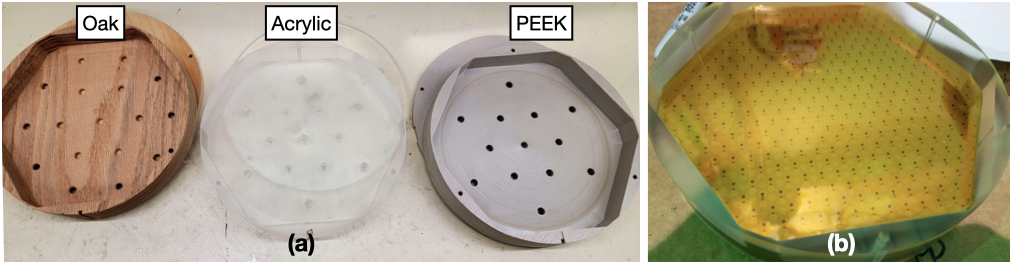
\includegraphics[width=0.99\textwidth]{figures/figures_edited_002.jpeg}
    \caption{(a) Sample containers ('hockey pucks') holding HGCAL silicon sensors for neutron irradiation at RINSC. 
    The deployed materials were wood (oak), acrylic, and PEEK.
    (b) An 8'' high-density HGCAL prototype silicon sensor inside an acrylic puck closed with a Kapton\texttrademark$~$foil.}
    \label{fig:Pucks_Arrayed}
  \end{center}
\end{figure}
The puck base has an outer diameter of \SI{18.6}{\centi\metre} that allows for a smooth fit inside the cylinder. 
Its interior of the puck is milled out in the profile of the silicon sensors with an additional clearance of \SI{1}{\milli\metre}. 
With these constraints the thinnest sections of the wall of the puck are slightly over \SI{1}{\milli\metre} thick which provides a difficult machining challenge.
The puck has a lid, made from the same material as the base, that matches the outer diameter of the base and provides a way to close the puck during handling.
Matching through holes in the base and lid allow for using nylon threaded rods and nuts to fasten the puck together. \newline
Kapton\texttrademark$~$foils were used to separate sensors in a stack such that no sensors are in direct contact with any rough surfaces (cf.~\ref{fig:Pucks_Arrayed}b).
In addition, antistatic foam was used for covering the top and bottom of the sensor-Kapton\texttrademark$~$stack serving as a cushion  against the walls inside the puck.
%Sensors were irradiated in batches of four, which required ten layers of Kapton\texttrademark$~$foils and three to four layers of antistatic foam. 
After preparation of the puck, the latter was inserted into the delivery cylinder.
In general, the silicon sensors should be kept at low temperatures during the irradiation in order to limit unwanted annealing.
For this purpose, the rest of the delivery cylinder was filled with 15-\SI{18}{\kilo\gram} of dry ice.
In order to monitor the temperature, PT1000 resistance temperature detectors (RTD) were inserted into the puck, at the front and the back face, to record the temperature throughout the irradiation for assessment of the expected sensor annealing during irradiation.\newline 
%Before the cylinder was closed, the RTD wires were routed through the vent holes in the removable cap, and were connected to a dedicated temperature readout system outside the beamport.
Once the cylinder had been fully packed, it was loaded onto a sled and inserted into the opening of the beamport.
It was then pushed all the way inside, the shutter was lowered, the lead plug was inserted into the opening of the beamport, and the setup was ready for irradiation.\newline
Representative temperature recordings during two different irradiation rounds are shown in~\ref{fig:Round_10_Temperature_Profile}.
\begin{figure}[!hbt]
  \begin{center}
    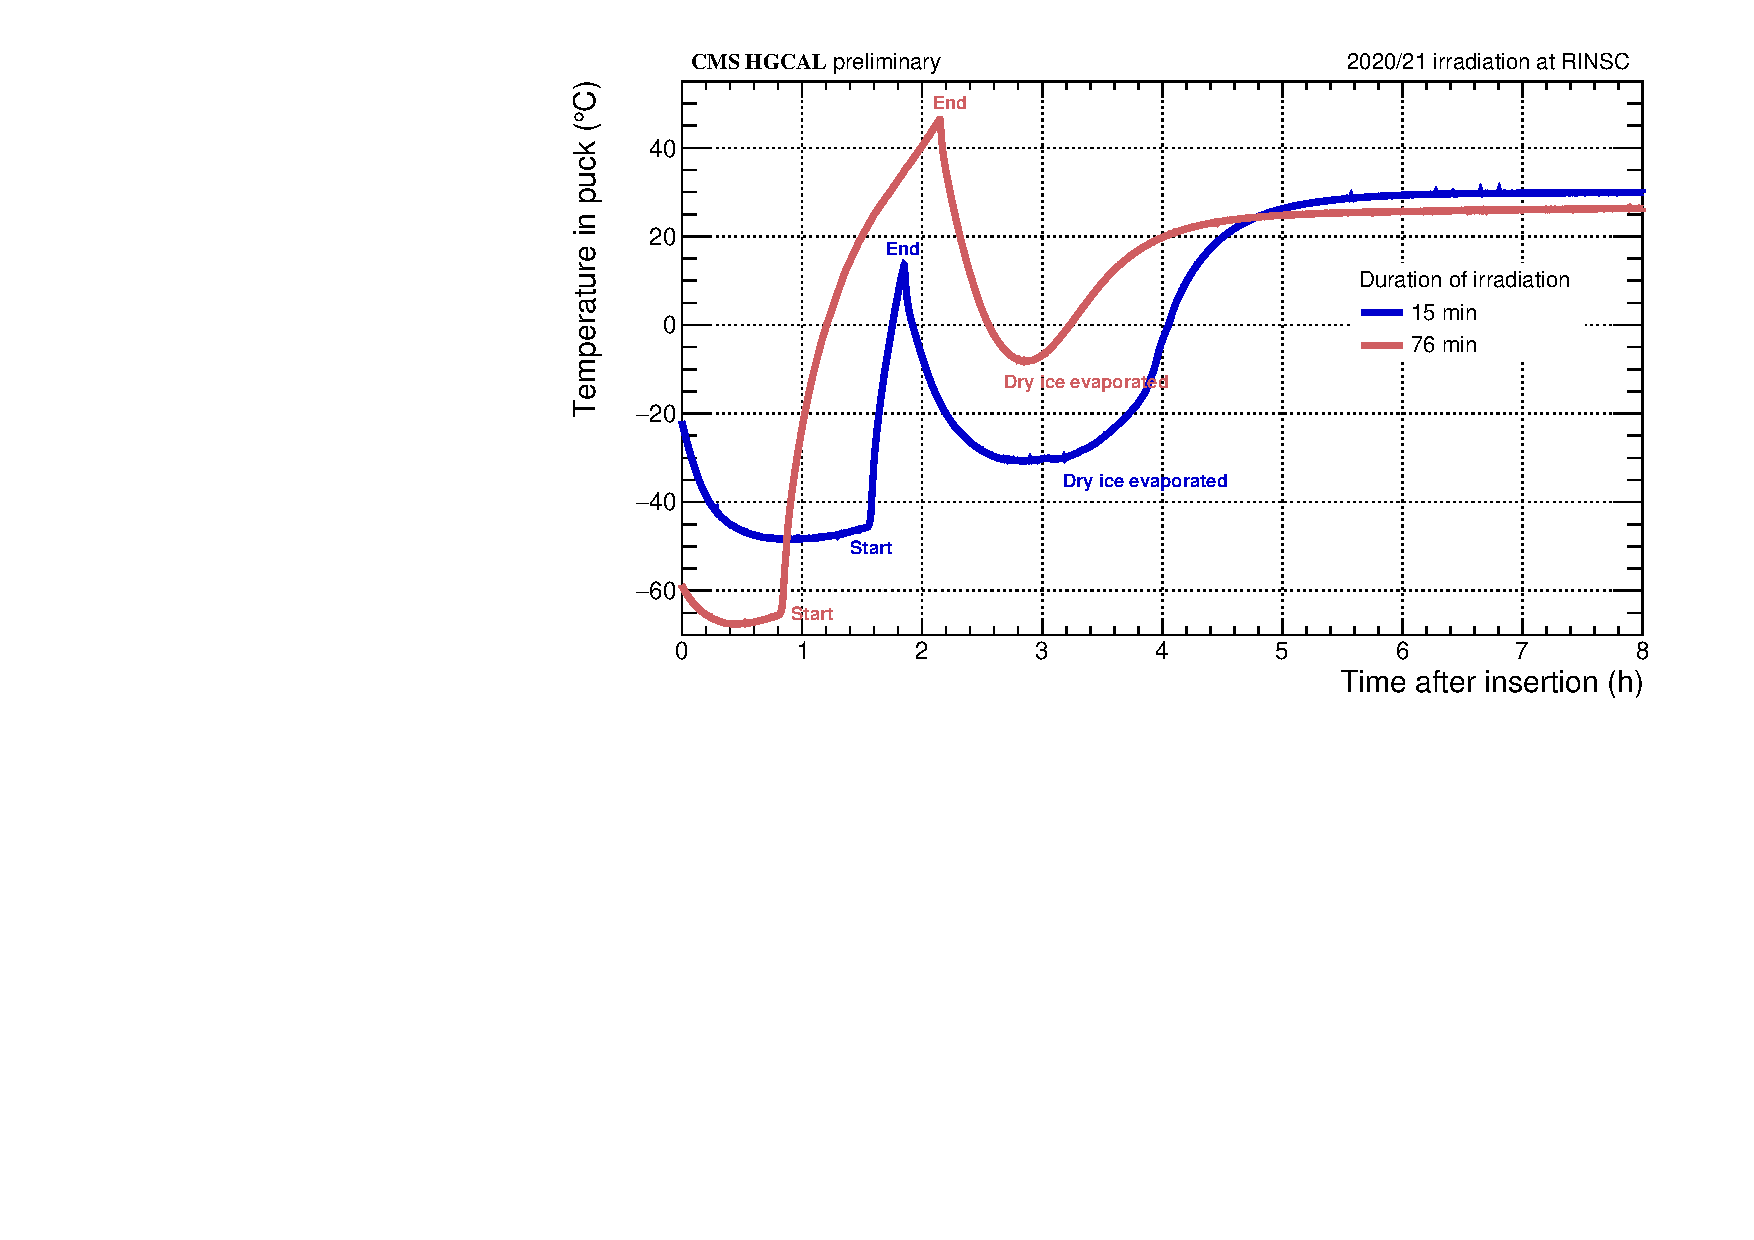
\includegraphics[width=0.69\textwidth]{plots/RINSC_temp/RINSC_temp.pdf}
    \caption{Representative temperature recordings during two of the RINSC irradiation rounds of HGCAL prototype silicon sensors. 
    The time when the irradiation was started and when it ended is indicated.
    The increase of the temperature towards its plateau coincides with the evaporation of the dry ice inside the delivery cylinder.
    }
    \label{fig:Round_10_Temperature_Profile}
  \end{center}
\end{figure}
During irradiation, the temperature rises significantly eventually reaching temperatures of a few \SI{+10}{\celsius} or more.
In fact, it was found that most of the dry ice was eventually consumed hereby.
Only after shutdown of the reactor, the temperature decreased again.
As a result, the annealing of the silicon sensors inside the beam port was in fact not negligible.
The corresponding annealing time at \SI{60}{\celsius} varied between a few minutes to a few hundred minutes for all the HGCAL silicon sensors irradiated at RINSC in 2020/21.
After \SI{24}{\hour} in the beamport after irradiation, the cylinder's radioactive levels have decayed sufficiently such that it could be safely extracted and the sensors be transferred into a storage freezer.

\subsection{Fluence Assessment}
In addition to the sensors, mechanical packing material, and temperature sensors, each puck contained a number of reference samples for measuring the fluence achieved during an irradiation round. 
Two different objects were found appropriate for measuring the fluences during this campaign: Reference silicon diodes from the D0 experiment, and ultrapure iron foils. 
The diodes were included inside the puck as close to the sensors as possible by encasing them in small plastic bags and taping them to the inside faces of the puck. 
By contrast, the iron foils were attached to the exterior of the cylinder for ease of removal and rapid counting. \newline
After irradiation, gamma spectra of the iron foils were measured at RINSC for derivation of the integrated fluence.
In addition, CV and IV measurements of the irradiated diodes were performed at Brown university to assess the depletion voltage, the associated dark current and ultimately the fluence assuming by the literature value for the current-related leakage current rate of $3.99\pm 0.03\cdot 10^{-17}~$A/cm at \SI{20}{\celsius}~\cite{moll:SiDamages}.\newline
%It was found empirically that the usage of commercially-available pin diodes saturated already at low fluences (below 4E14) and thus were not found to be particularly useful. 
The reference silicon diodes are most useful for the lower to medium range of the targeted fluences,  where their depletion voltage was well within the measurement range ($<\SI{1000}{\volt}$).
For higher fluences, full depletion of the silicon diodes could not be reached, and the gamma ray spectra derived from the iron foils are considered more reliable.
\ref{table:irrads} in~\ref{appendix:irrad_rounds} shows the estimated actual fluences from those reference samples.\newline
In order to improve the accuracy of the fluence assessment, future irradiation of HGCAL silicon wafers at RINSC will include iron foils inside the puck as well as additional test structures of HGCAL silicon sensors.
\section{Electrical Characterisation of Silicon Sensors}
\label{sec:setup}
The experimental setup and the procedure for the electrical characterisation of silicon sensors is presented in this section.
Although those tests were conducted at different locations, the following description is limited to the particular setup at CERN from which most of the results of this work were obtained.

\subsection{Setup at CERN}
\label{subsec:setup_alps}
At CERN, the S200FA probe station produced by Wentworth Laboratories Ltd. was in use for the electrical characterisation of neutron-irradiated silicon sensors. 
It is referred to as "Automatic-Low-Temperature Probe Station" (ALPS) because of its temperature-controlled chuck (produced by Systems att, C200-40 model) that can reach temperatures down to \SI{-40}{\celsius} and its programmable movements.
Apart from the power supply and meters, all relevant components were installed inside ALPS, see \ref{fig:ALPS_setup}.
\begin{figure}[h]
	\centering
	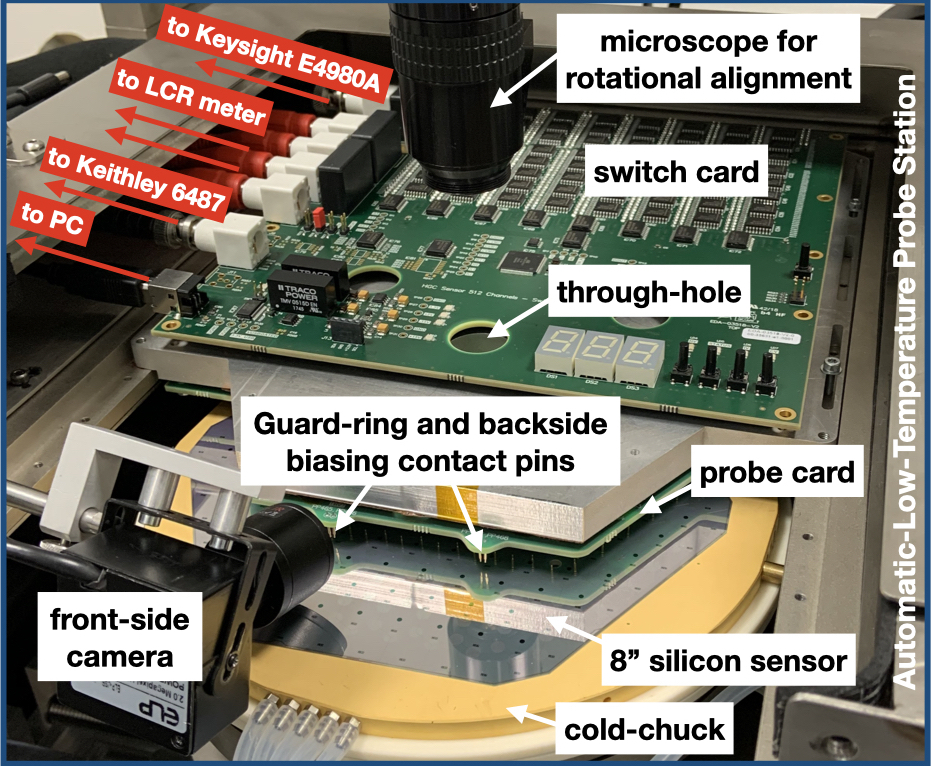
\includegraphics[width=0.75\textwidth]{figures/ALPS_photo_edit.jpeg}
	\caption{
		Silicon sensor right before connecting to the switch- and probe-card ARRAY system inside the Automatic-Low-Temperature-Probe Station (ALPS) at CERN for the testing of neutron-irradiated CMS HGCAL silicon sensor prototypes.
		The probe station was closed and flushed with dry air during the testing to prevent the formation of ice.
		}
		\label{fig:ALPS_setup}
	\end{figure}
The silicon wafers were first placed on the chuck and then connected to the probe- and switch-card based ARRAY system~\cite{pitters:array2019}.
Through-holes in the cards and the probe station's microscope  enable sufficient sensor-to-pin alignment. 
The high voltage from the Keithley 2410 power supply was provided to the chuck and to the sensor's backside.
Two probe cards specific for the high- and for the low-density sensor layouts had been designed and manufactured for the tests.
Exploiting the availability of a dedicated pad, also the guard ring could be connected through pins on the probe cards.
The switch card was operated with a bias resistance (R$_\text{bias}$) of \SI{1}{\mega\ohm} and a high voltage resistance (R$_\text{HV}$) of \SI{12}{\kilo\ohm}.
In this configuration, the ARRAY system is designed to withstand total leakage currents up to $\mathcal{O}(\SI{1}{\milli\ampere})$ and per-pad currents up to \SI{10}{\micro\ampere}.
Cooling the neutron-irradiated sensors down to \SI{-40}{\celsius} was therefore imperative.
The spatial variation of the chuck's temperature profile at this temperature amounts to $\pm\SI{0.5}{\celsius}$, cf.~\ref{appendix:chuck_temp}, whereas fluctuations with time are found to be negligible. 
In order to prevent the formation of ice, the probe station had to be flushed with dry air. 
With total currents at the order of $\mathcal{O}(\SI{1}{\milli\ampere})$, the voltage drop at R$_\text{HV}$ for the testing of neutron-irradiated sensors is non-negligible and is corrected for in \ref{sec:results}.
The voltage at the silicon pad under test is referred to as "effective bias voltage" in this work.
Per-pad leakage currents were measured with a Keithley 6487 picoammeter, whereas total currents were measured directly with the Keithley 2410 power supply.
A Keysight E4980A LCR meter was operated at a frequency (f$_\text{LCR}$) of \SI{2}{\kilo\hertz} for the inference of the per-pad impedance.
This particular frequency was chosen to minimise the error associated to the capacitance~\cite{pitters:array2019}.
It was found empirically that the impact on the end capacitance is negligible whereas the derived depletion voltages are increased by about \SI{10}{\percent} when reducing f$_\text{LCR}$ to \SI{500}{\hertz}. 

\subsection{Measurement Procedure}
\label{subsec:setup_procedure}
After connecting the sensor to the probecard, per-pad leakage currents as a function of the bias voltage (IV) for the full sensor were measured first, preceded by a per-pad capacitance vs. bias voltage assessment (CV).
After each iteration over all pads a given bias voltage, voltages were incremented up to \SI{850}{\volt}, whereby the exact choice depended on the measurement type and on the sensor thickness, or up to a maximum total leakage current of \SI{2}{\milli\ampere}.  
Pads whose leakage currents exceeded \SI{5}{\micro\ampere} were not measured any further and in particular were excluded from the subsequent CV.
The entire characterisation sequence is fully automatised as a LabView-based program (HexDAQ version 1.5.1~\cite{labview_hexdaq}).
Including voltage ramps and settling times, IV measurements of low-density sensors took about \SI{1.5}{\hour} (CV: \SI{2.5}{\hour}), whereby the duration was about twice as long for high-density sensors.
IV and CV measurements were performed both before and after a beneficial annealing for \SI{80}{\min} at \SI{60}{\celsius}\footnote{Corresponding to about two weeks at room temperature.}
\section{Results}
\label{sec:results}
The results of the electrical characterisation of the neutron-irradiated HGCAL silicon pad sensor prototypes are presented in this section. 
\ref{subsec:leakagecurrents} focuses on the discussion of leakage currents (\emph{IV}) whereas \ref{subsec:Udep} addresses the findings of the capacitance (\emph{CV}) and depletion voltage assessments. 
The presentation of the results is complemented in \ref{subsec:discussion} with a discussion on the limitations in their interpretability and on the drawn conclusion.

\subsection{Leakage Current}
\label{subsec:leakagecurrents}
\begin{figure}
	\captionsetup[subfigure]{aboveskip=-1pt,belowskip=-1pt}
	\centering
	\begin{subfigure}[b]{0.49\textwidth}
		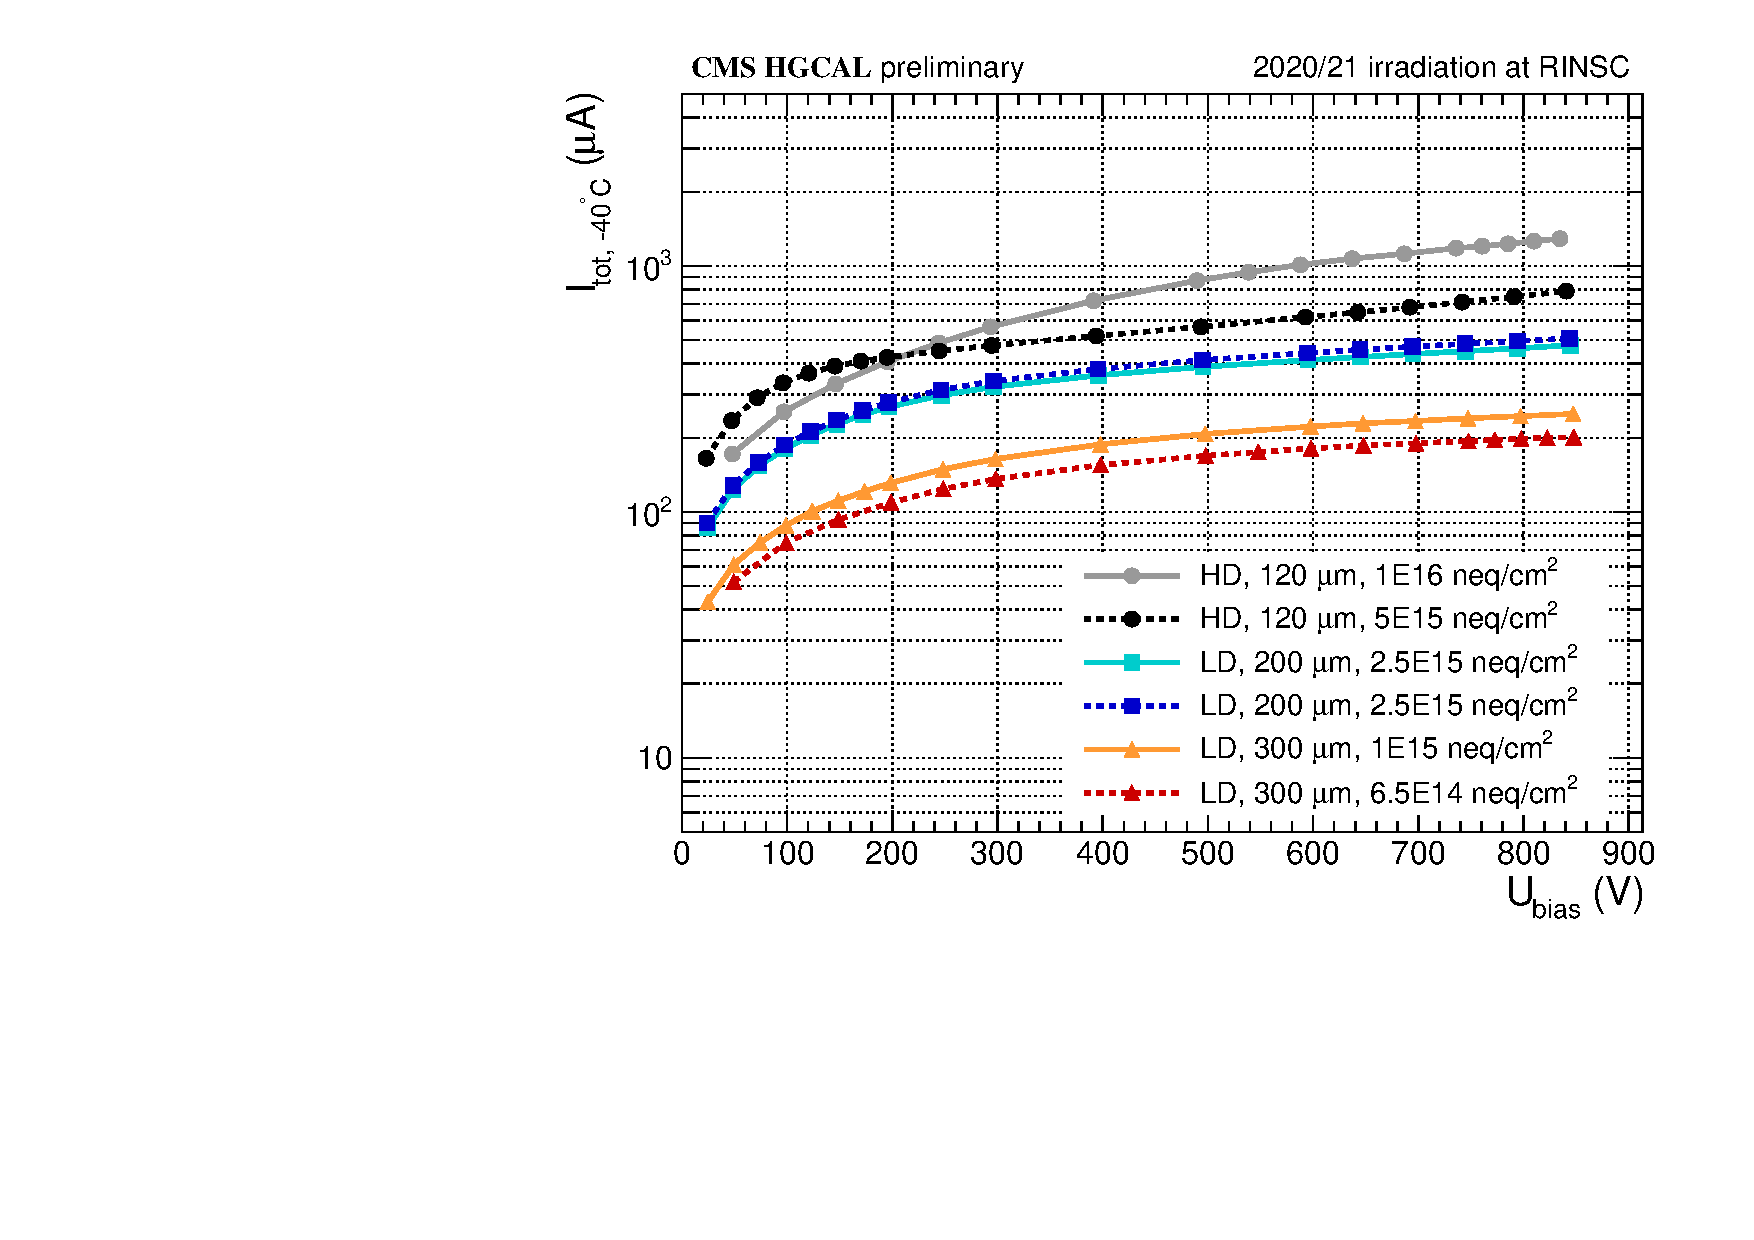
\includegraphics[width=0.999\textwidth]{plots/total_iv/total_current_IV.pdf}
		\subcaption{
		}
		\label{plot:tot_IV_good}
    \end{subfigure}
    \hfill
    \begin{subfigure}[b]{0.49\textwidth}
        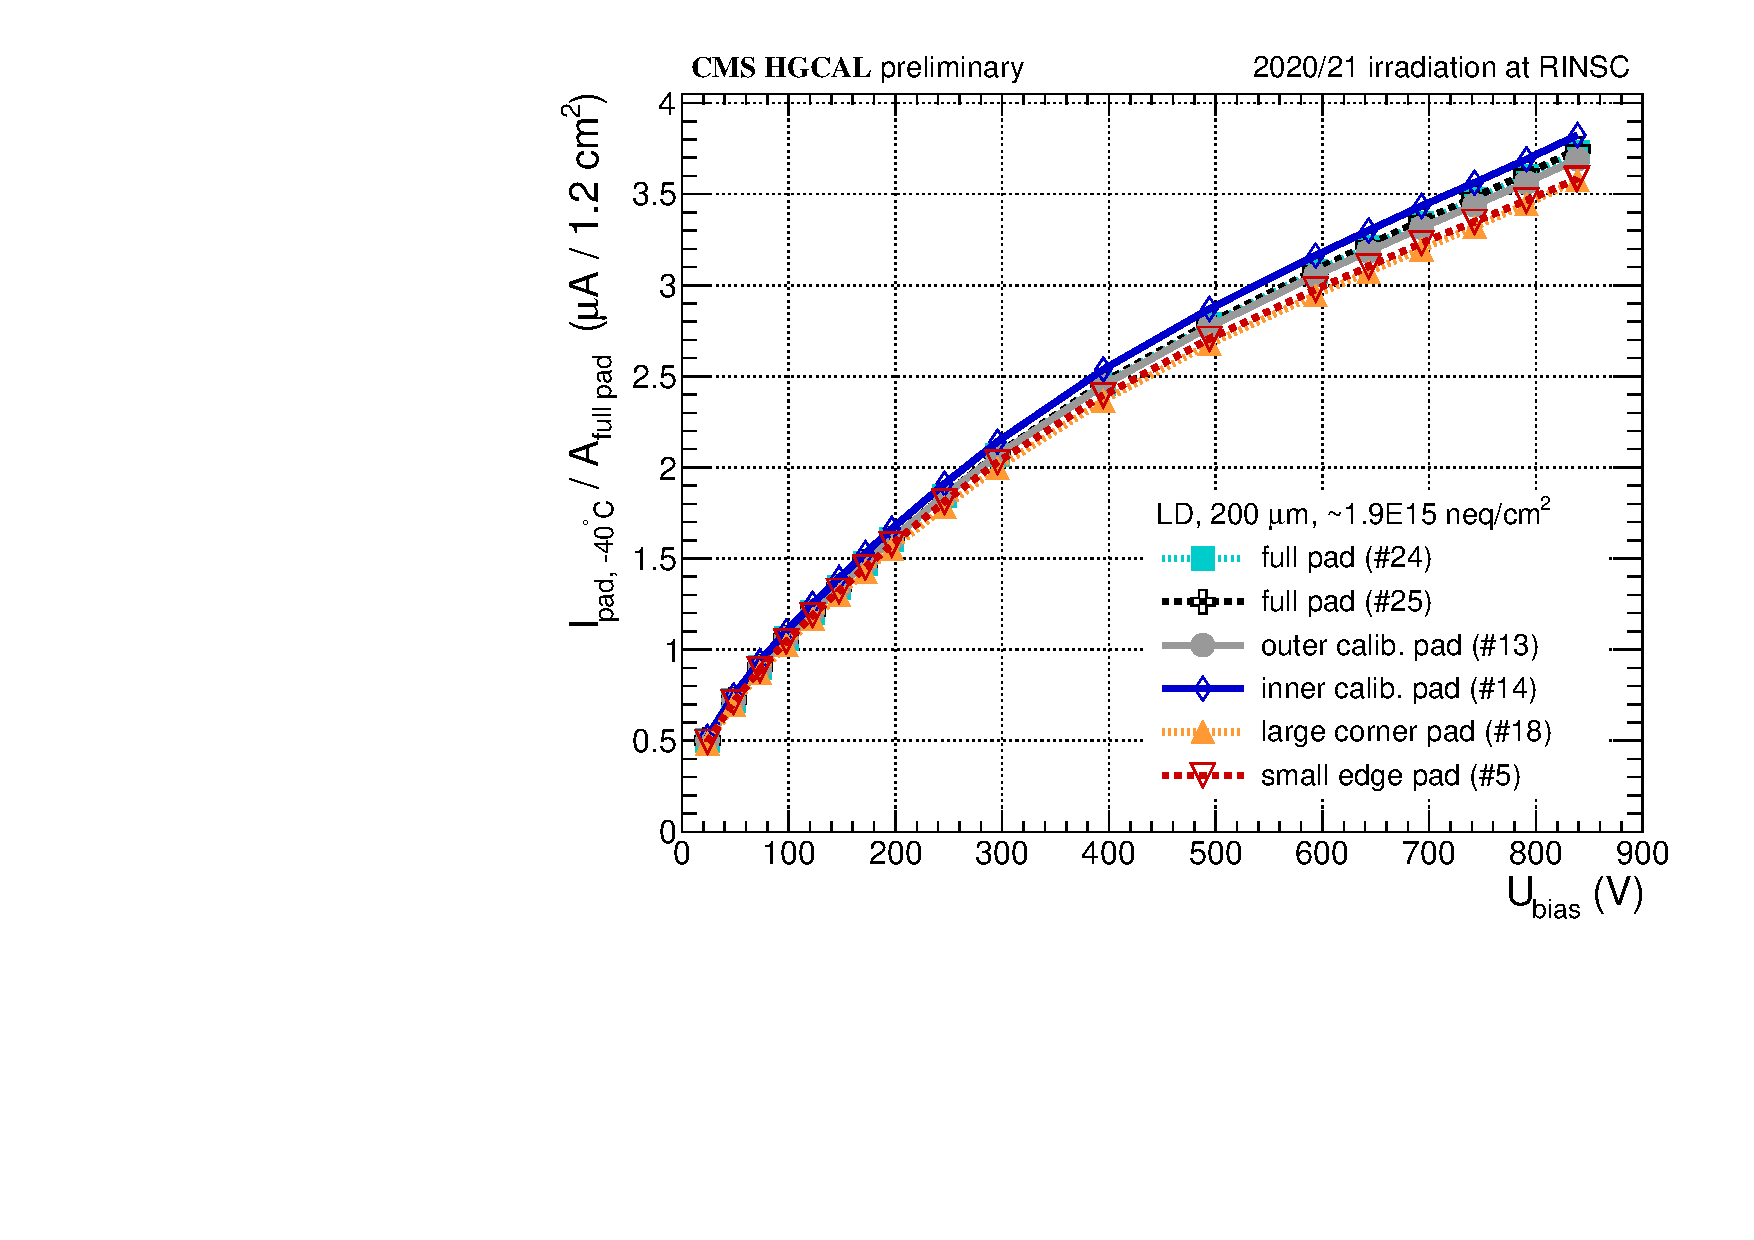
\includegraphics[width=0.999\textwidth]{plots/channel_iv/channel_IV_sensors_channels.pdf}
        \subcaption{
        }
        \label{plot:pad_IV_channels}
    \end{subfigure}

	\caption{
		(a) Total leakage currents after irradiation (without additional thermal annealing) for two representative example sensors. 
		Currents were measured at \SI{-40}{\celsius} ($\text{I}_\text{tot, \SI{-40}{\celsius}}$) and at different effective bias voltages ($\text{U}_\text{bias}$). 
        (b) Per-pad leakage currents normalised to the area of full hexagonal pads as a function of the effective bias voltage for different pads with different geometries on one example sensor.
	}
\end{figure}
The total leakage current, interpreted as the dark current of a full silicon sensor, is defined as the current flowing through the high-voltage resistor R$_\text{HV}$ (cf. Figure 2 in~\cite{pitters:array2019}).
As it is exemplified for two prototype sensors in \ref{plot:tot_IV_good}, the total leakage current did not exhibit indications of breakdowns and stayed well below the ARRAY system's compliance of \SI{2}{\milli\ampere} for most of the irradiated sensors that were tested up to \SI{850}{\volt} at \SI{-40}{\celsius}.
Irreversible discharges are undesired but in fact occurred for a handful of the tested sensors where the total leakage current during electrical characterisation suddenly increased and exceeded the \SI{2}{\milli\ampere} limitation.
Whereas one half of those instances could be traced back to mechanical damages, e.g.$~$induced during the transport or sensor handling, the other half hinted at the presence of a minor flaw in the HGCAL silicon sensor design.
The latter ultimately lead to a design modification with which the risk of discharges in the future should be minimised\footnote{More than 50 prototype sensors with the improved design have been characterized with voltages up to \SI{850}{\volt} in the meantime. None have shown discharges thus far.}.
Results of the affected sensors are not discussed further in this work.
\ref{plot:pad_IV_channels} shows the per-pad leakage current as a function of the effective bias voltage for adjacent pads on one representative low density sensor irradiated to intermediate fluences of $\sim 1.9\cdot 10^{15}~\neqcm$.
The data demonstrate that, in good approximation, the leakage current of a pad after irradiation scales with its volume.
The relative increase from \SI{600}{\volt} to \SI{800}{\volt} remains well below \SI{150}{\percent}, again not showing indications of sensor breakdowns.
The beneficial effect of annealing on the leakage current has been studied in more detail for a sensor which was not exposed to high temperatures during irradiation.
The measured IV curves after different annealing times are shown for a representative pad in \ref{plot:annealing_IV}.
\begin{figure}
	\captionsetup[subfigure]{aboveskip=-1pt,belowskip=-1pt}
	\centering
	\begin{subfigure}[b]{0.49\textwidth}
		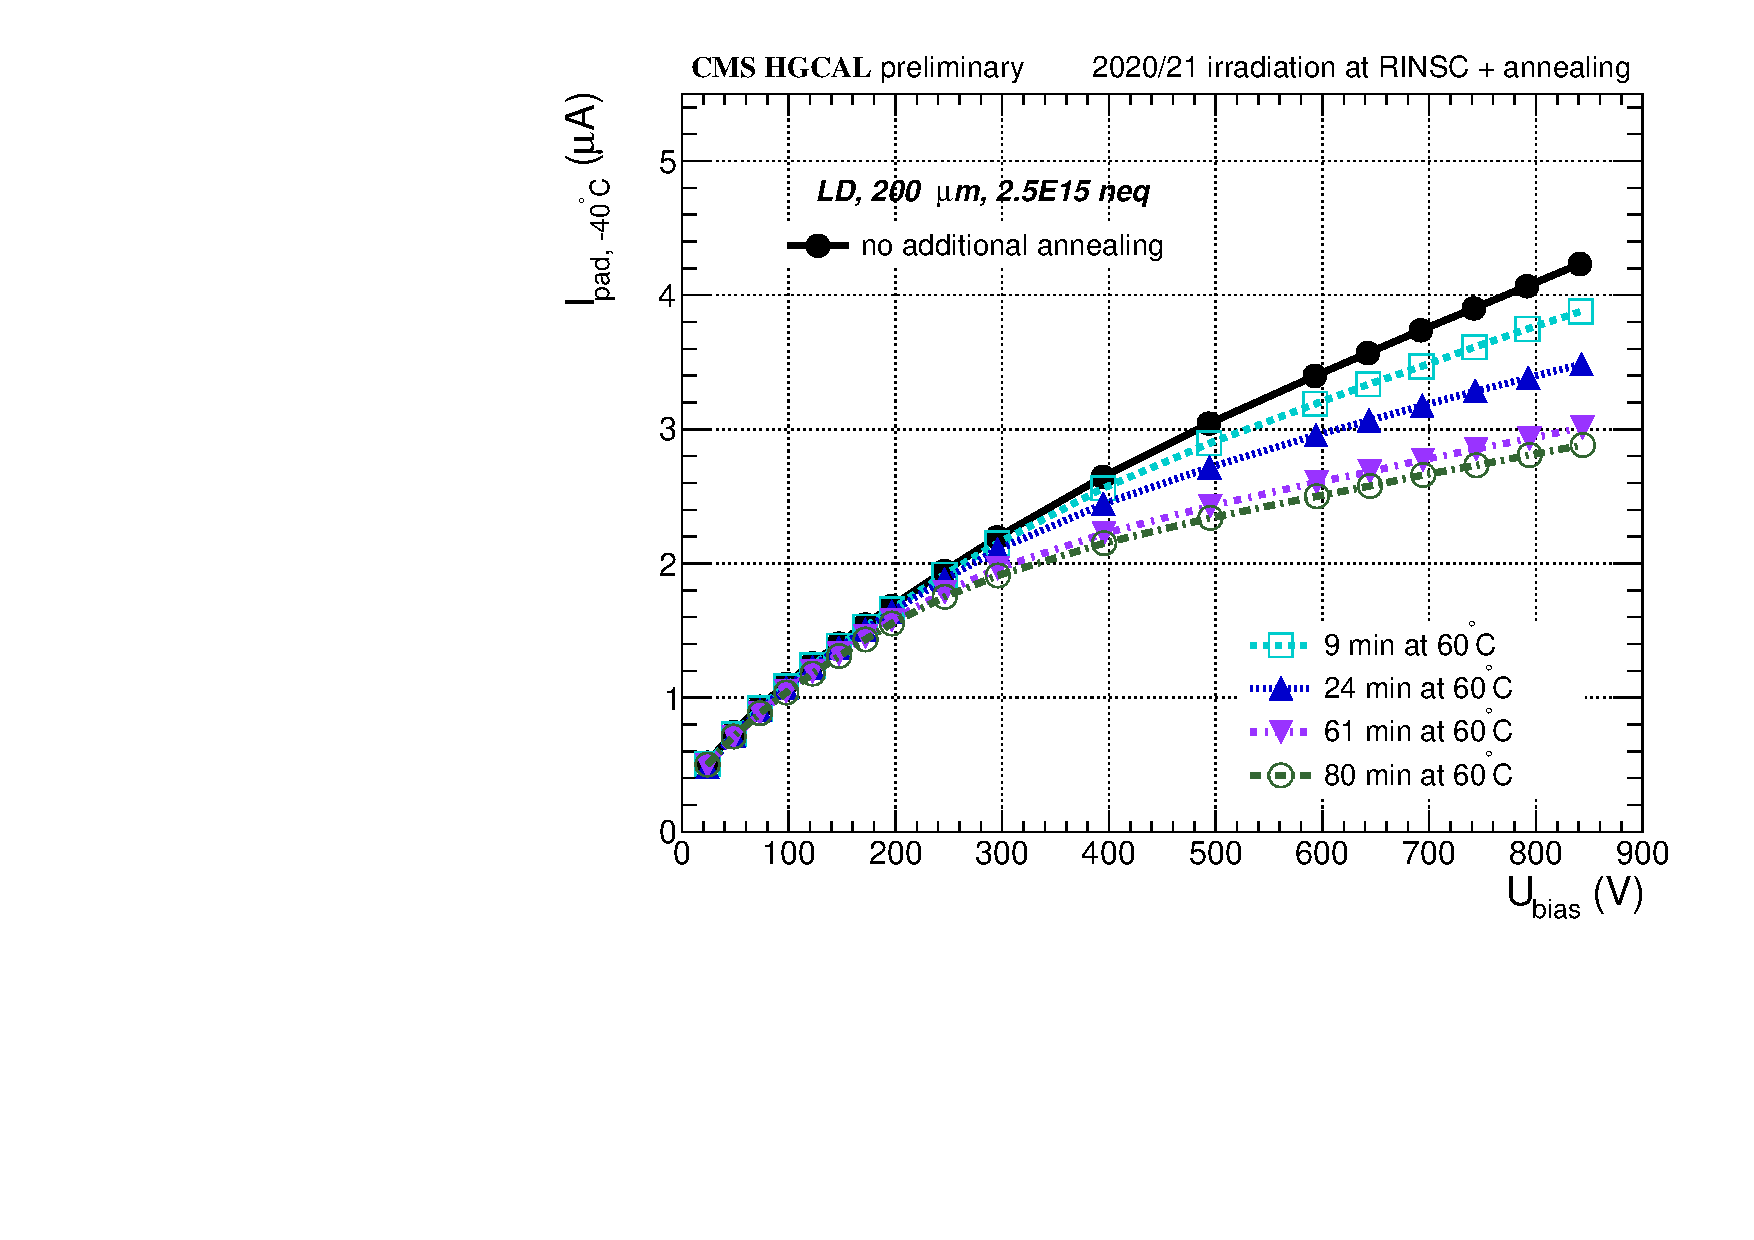
\includegraphics[width=0.999\textwidth]{plots/annealing_iv/annealing_IV_ch24.pdf}
		\subcaption{
		}
		\label{plot:annealing_IV}
	\end{subfigure}
	\hfill
	\begin{subfigure}[b]{0.49\textwidth}
		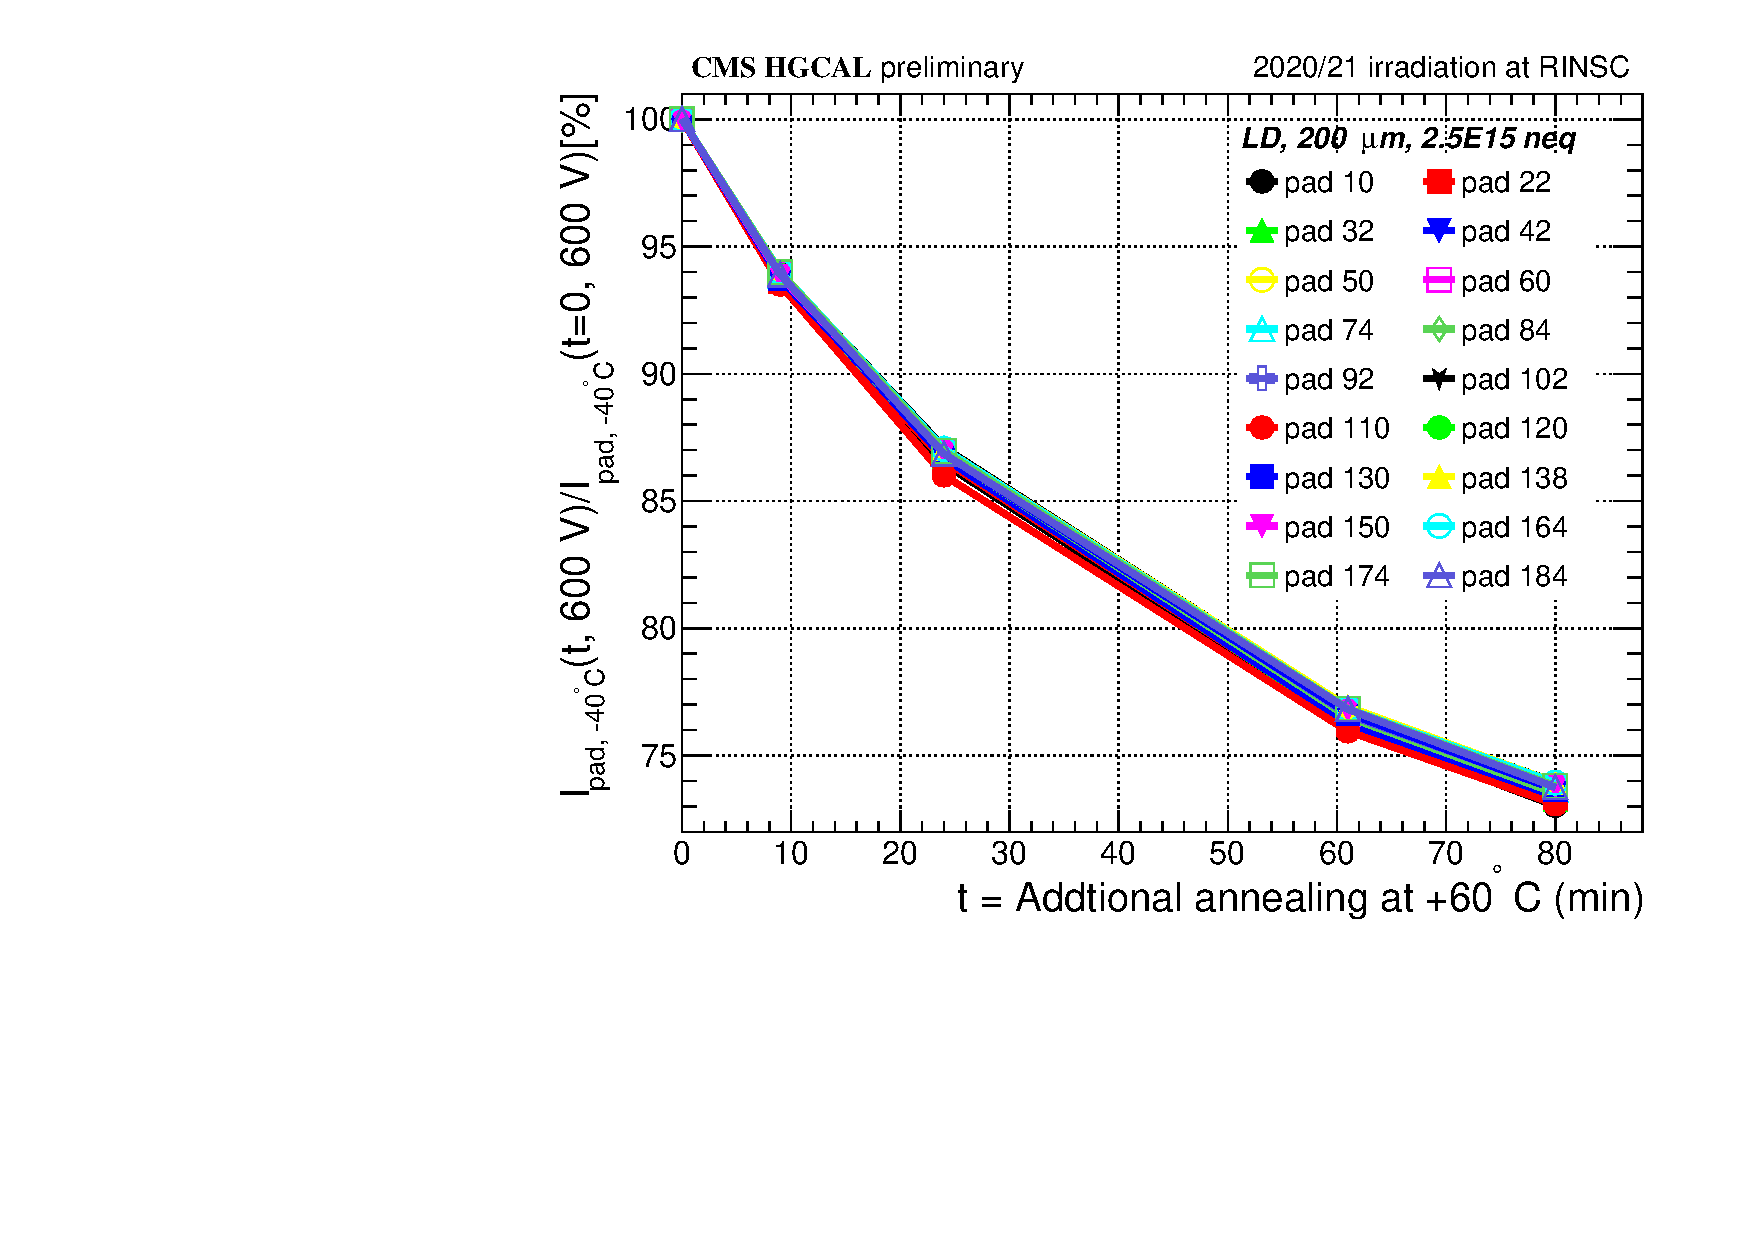
\includegraphics[width=0.999\textwidth]{plots/annealing_iv/annealing_current.pdf}
		\subcaption{
		}
		\label{plot:annealing_current}
	\end{subfigure}    

	\caption{
		(a) IV-curves of a representative full hexagonal pad for different annealing durations for a \SI{200}{\micro\metre} low-density prototype sensor irradiated to approximately 2.4$\cdot 10^{15}~\neqcm$.
        (b) Decrease of the per-pad leakage current (interpolated to $U_\text{bias}=\SI{600}{\volt}$) as a function of the annealing time at \SI{60}{\celsius} for a subset of full hexagonal pads that are uniformly distributed over the full sensor.
	}
\end{figure}
For bias voltages beyond full depletion, per-pad leakage currents at \SI{600}{\volt} are reduced systematically by \SI{25}{\percent} after \SI{80}{\minute} at \SI{60}{\celsius}, cf.~\ref{plot:annealing_current}.
Given the simultaneous reduction in the depletion voltage, cf.~\ref{plot:annealing_CV}, leakage currents around full depletion are even reduced further.
Altogether, we observe the expected proportionality of the per-pad leakage current density to the anticipated fluence that the sensors were exposed to.
The proportionality for current densities interpolated to an effective bias voltage of \SI{600}{\volt}, which is well above full depletion for most of the investigated sensors, and extrapolated to HGCAL's foreseen operation temperature of \SI{-30}{\celsius} is displayed in \ref{plot:alpha_600}.
\begin{figure}
	\captionsetup[subfigure]{aboveskip=-1pt,belowskip=-1pt}
	\centering
    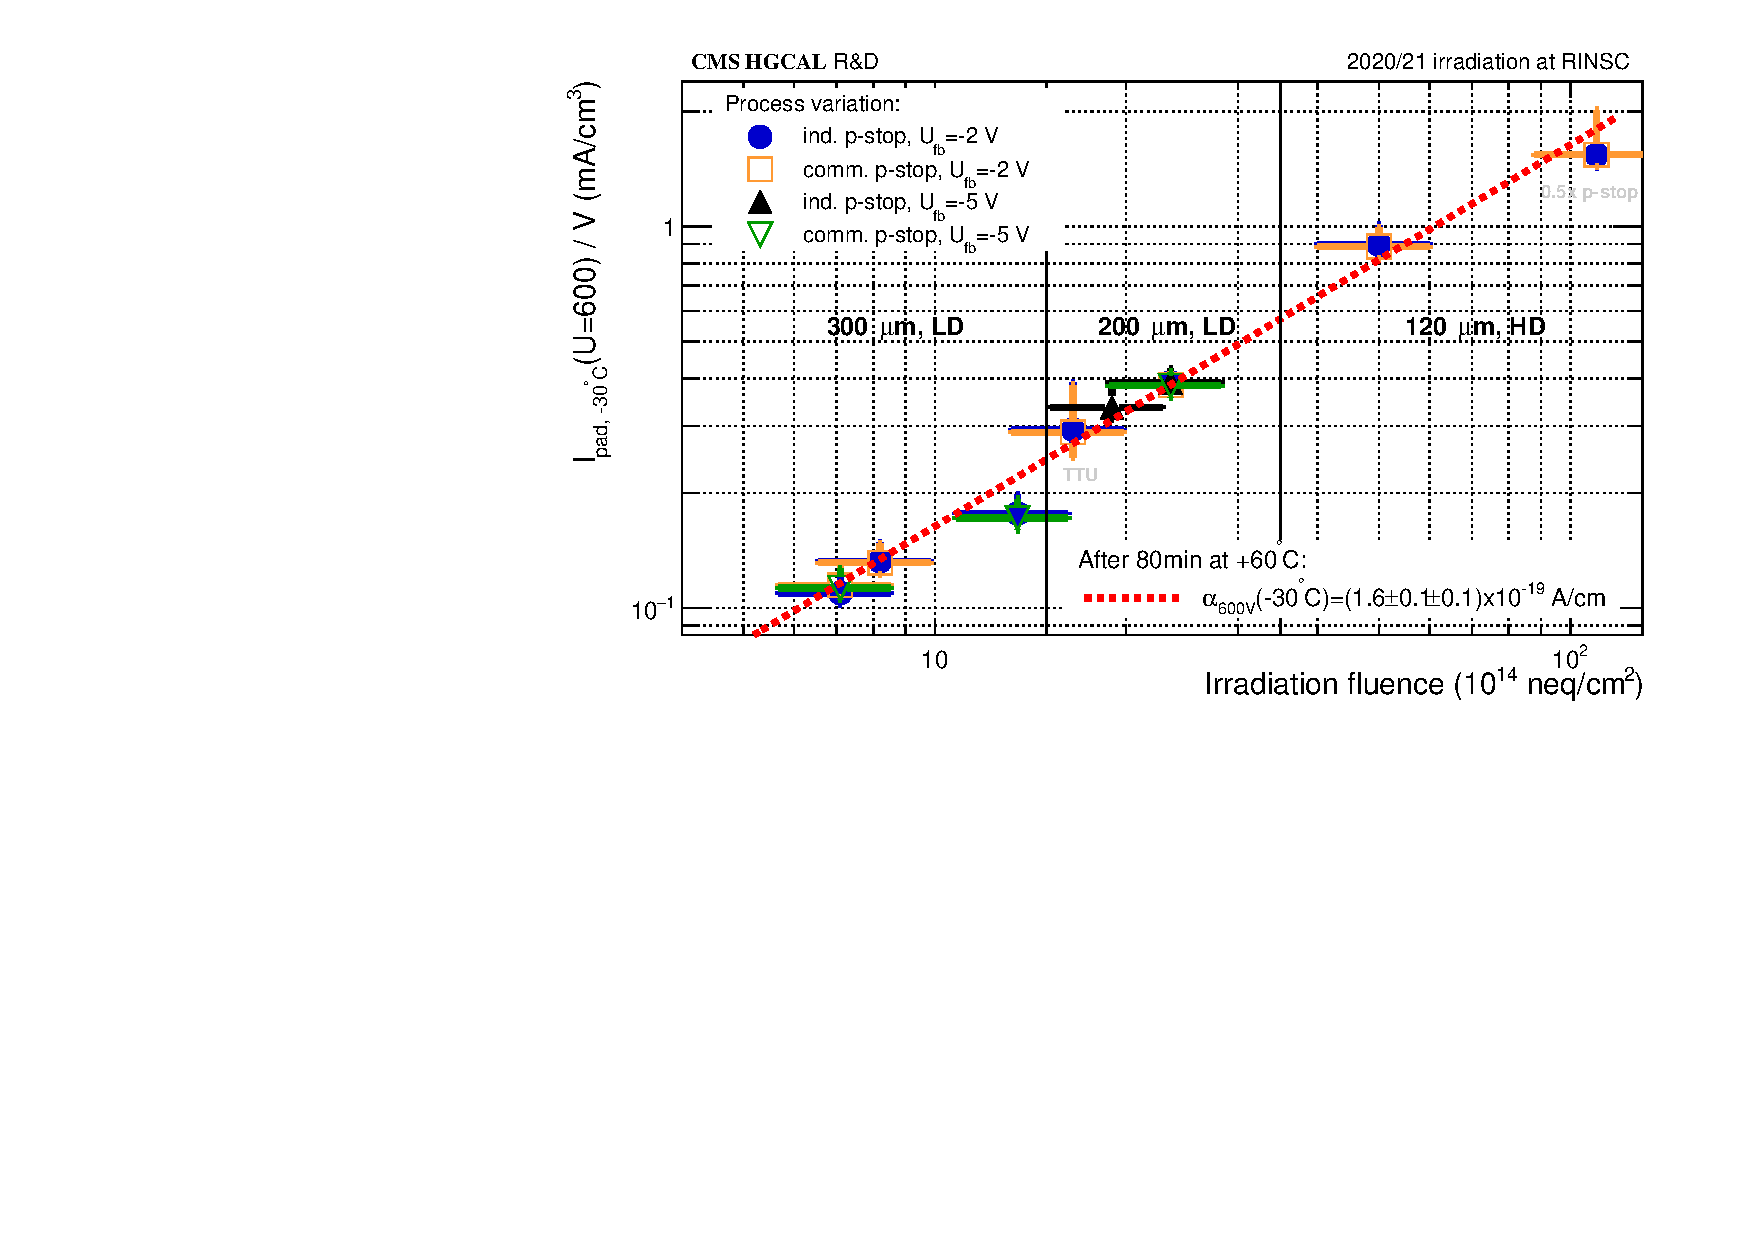
\includegraphics[width=0.69\textwidth]{plots/alpha/alpha_600V.pdf}
	\caption{
		Volume-normalised per-pad leakage currents interpolated to an effective bias voltage of \SI{600}{\volt} as a function of the fluence that they were exposed to.
        The quoted currents were measured after additional annealing at \SI{60}{\celsius}, and are scaled to HGCAL's foreseen operation temperature of \SI{-30}{\celsius}.
		"0.5x p-stop" denotes HD sensors with half the p-stop concentration.
		"TTU" denotes the measurements of \SI{120}{\micro\meter} HD sensors conducted with a setup, analogous to the one described in~\ref{subsec:setup_alps}, at Texas Tech University. 
		Those exhibit overall consistency with the measurements conducted with the setup at CERN.
		}
	\label{plot:alpha_600}
\end{figure}
As expected~\cite{MOLL199987}, the current-related damage rate ($\alpha$) is found to be independent of the tested silicon material properties investigated in this work.
However, the numerical result for $\alpha$ scaled to room temperature, $\alpha_\text{600V}(\SI{+20}{\celsius})=\left(3.2\pm 0.2\pm 0.2\right)\cdot 10^{-17}~$A/cm, is about \SI{20}{\percent} less than the literature value~\cite{moll:SiDamages}.
Among other contributing factors, this could indicate a systematic overestimate of the fluence at the RINSC irradiation facility.\newline 
Interestingly, even after correction for the chuck temperature non-uniformity, per-pad leakage current densities across a sensor at a fixed voltage vary significantly by $\mathcal{O}(10~\%)$.
The associated current profiles are present both before (cf. \ref{plot:iv_hexplot_3009,plot:iv_hexplot_0541_04,plot:iv_hexplot_1013}) and after additional annealing (cf. \ref{plot:iv_hexplot_3009_annealed,plot:iv_hexplot_0541_04_annealed,plot:iv_hexplot_1013_annealed}).
Furthermore, they are consistent between sensors that had been irradiated simultaneously in the same puck.
Hence, this circumstance is interpreted as evidence for the presence fluence profile within the beam port of the irradiation facility at RINSC.
It is noted that this fluence profile can reasonably well be approximated as a Gaussian with a width of $\sigma\sim\SI{10}{\centi\metre}$.
\begin{figure}
	\captionsetup[subfigure]{aboveskip=-1pt,belowskip=-1pt}
	\centering
	\begin{subfigure}[b]{0.32\textwidth}
		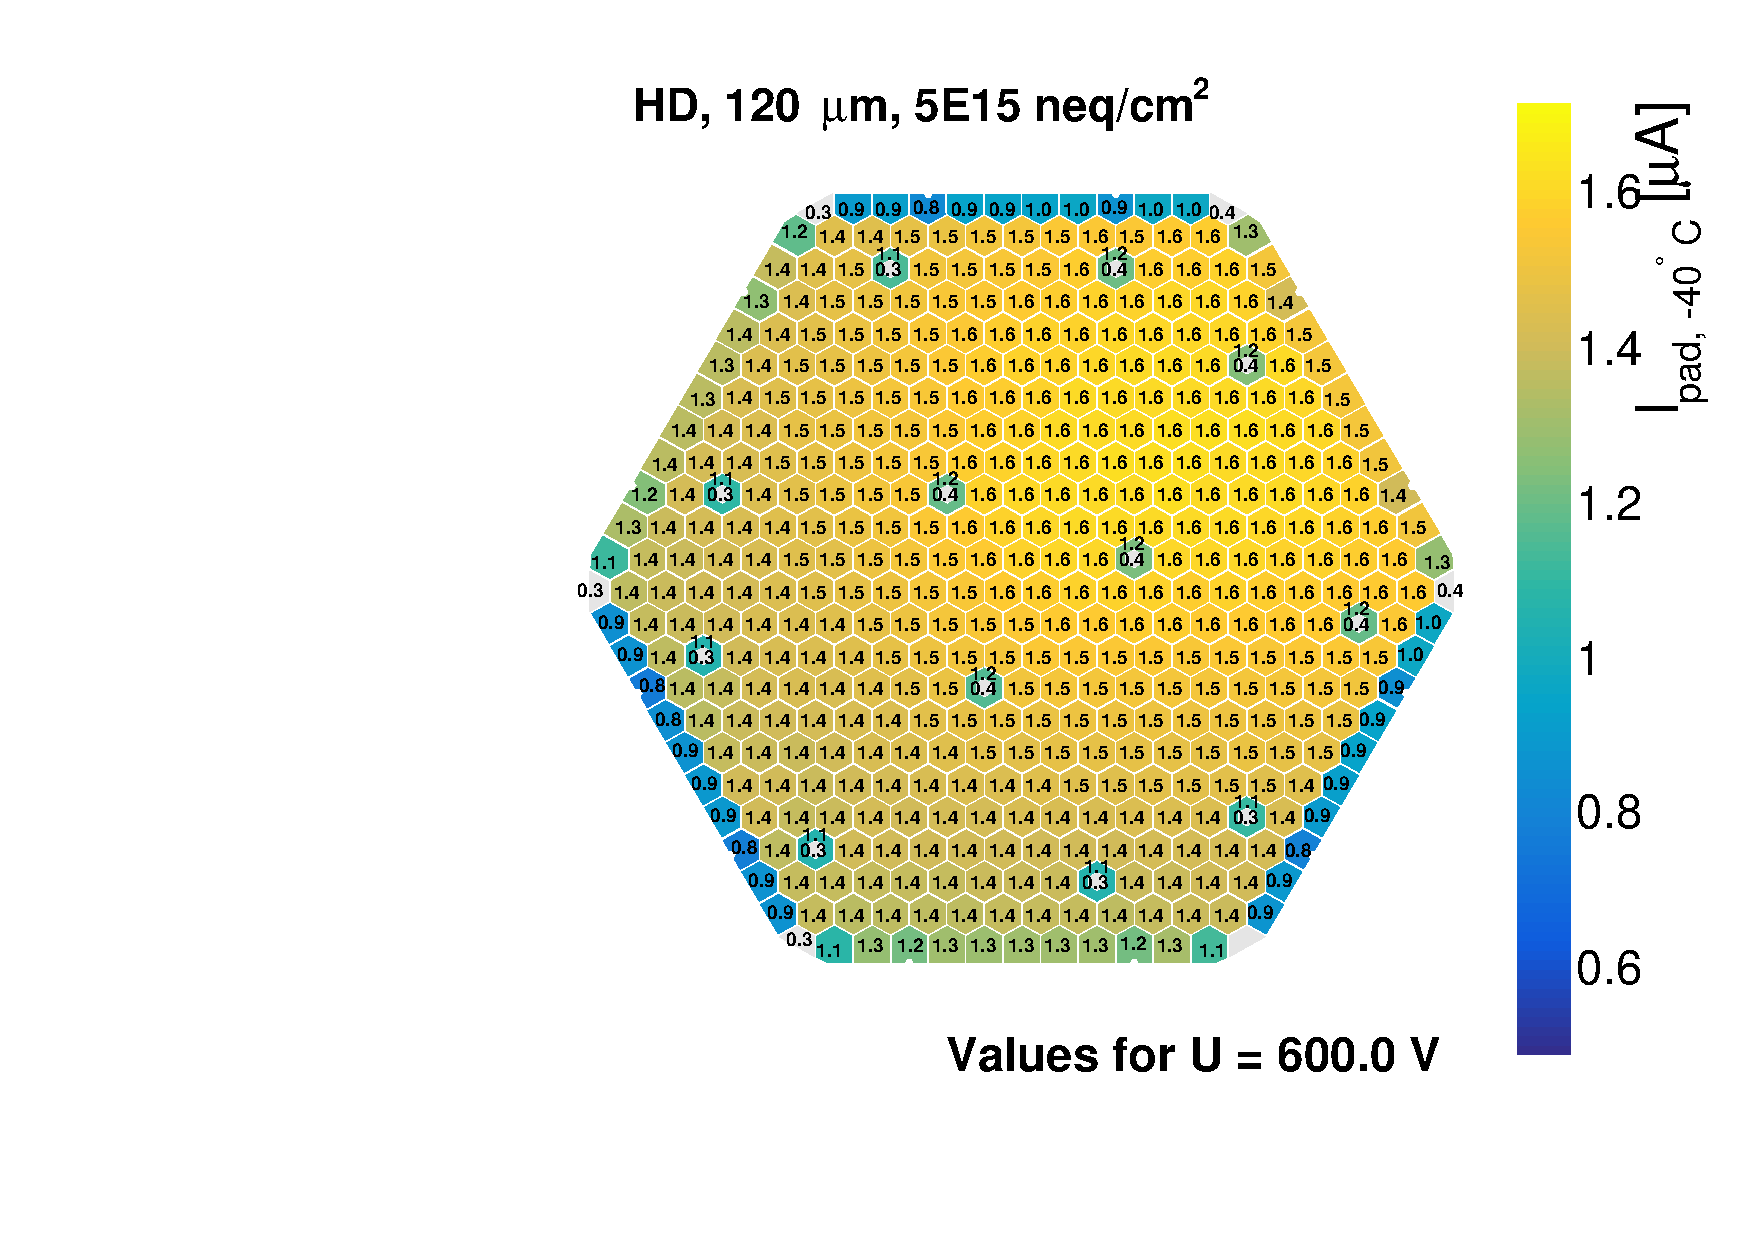
\includegraphics[width=0.999\textwidth]{plots/iv_hexplots/3009.pdf}
		\subcaption{
		}
		\label{plot:iv_hexplot_3009}
	\end{subfigure}
	\hfill
	\begin{subfigure}[b]{0.32\textwidth}
		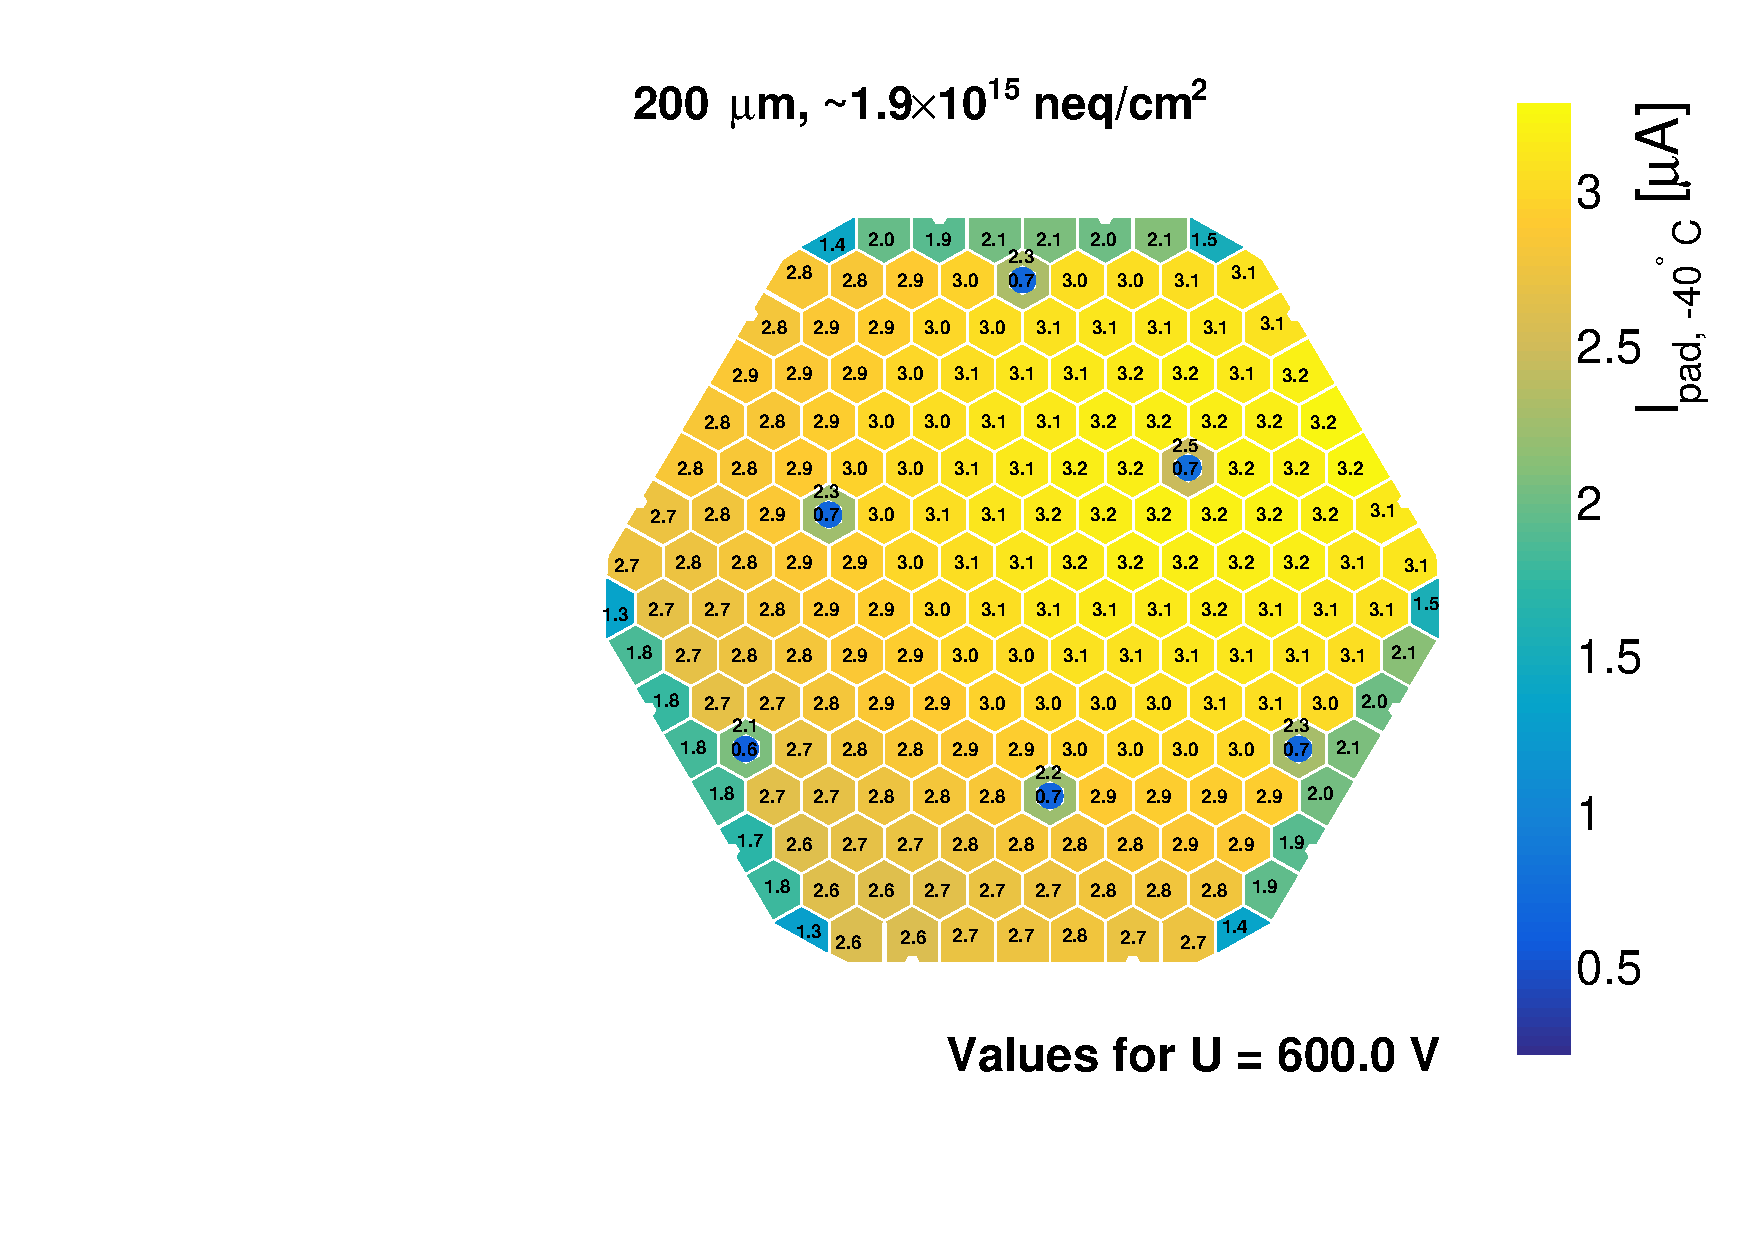
\includegraphics[width=0.999\textwidth]{plots/iv_hexplots/0541_04.pdf}
		\subcaption{
		}
		\label{plot:iv_hexplot_0541_04}
	\end{subfigure}
	\hfill	
	\begin{subfigure}[b]{0.32\textwidth}
		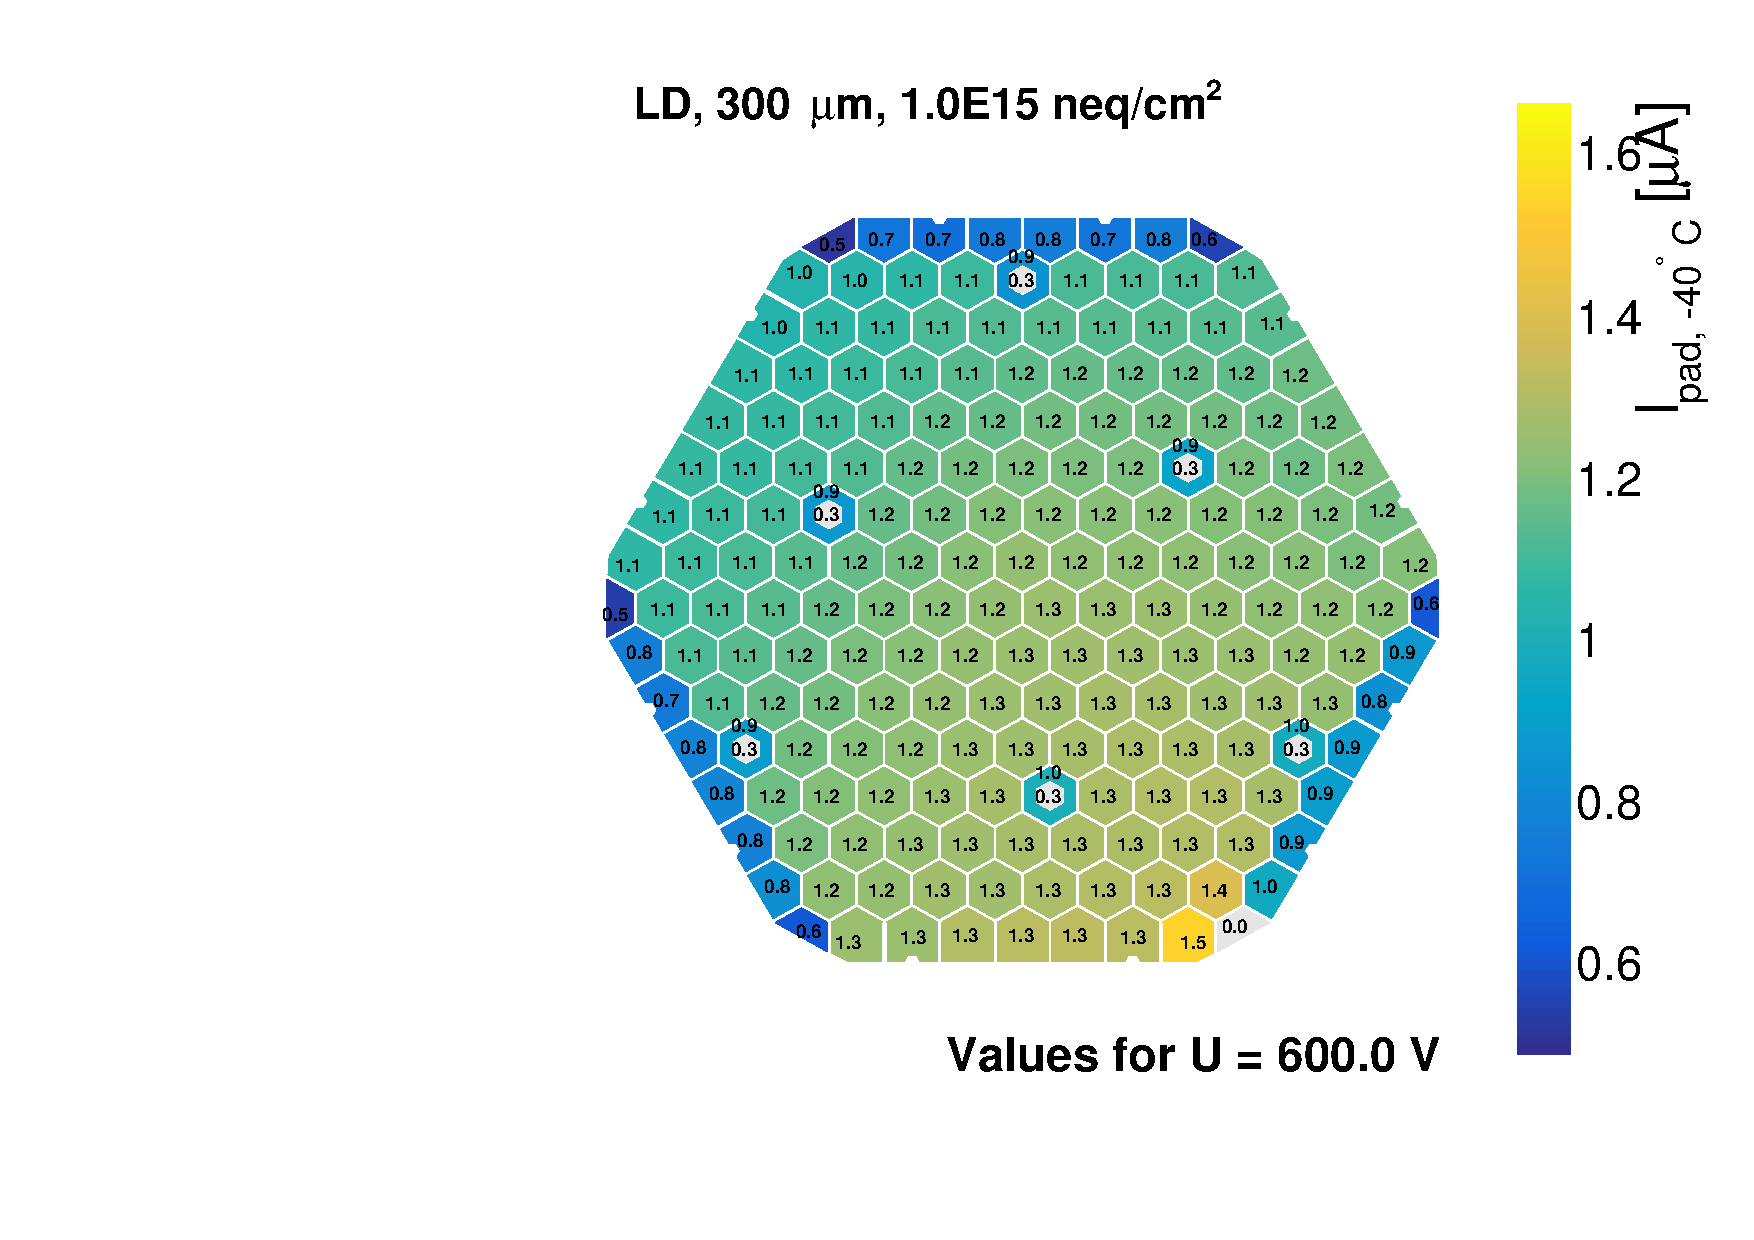
\includegraphics[width=0.999\textwidth]{plots/iv_hexplots/1013.pdf}
		\subcaption{
		}
		\label{plot:iv_hexplot_1013}
	\end{subfigure}
    \hfill
	\begin{subfigure}[b]{0.32\textwidth}
		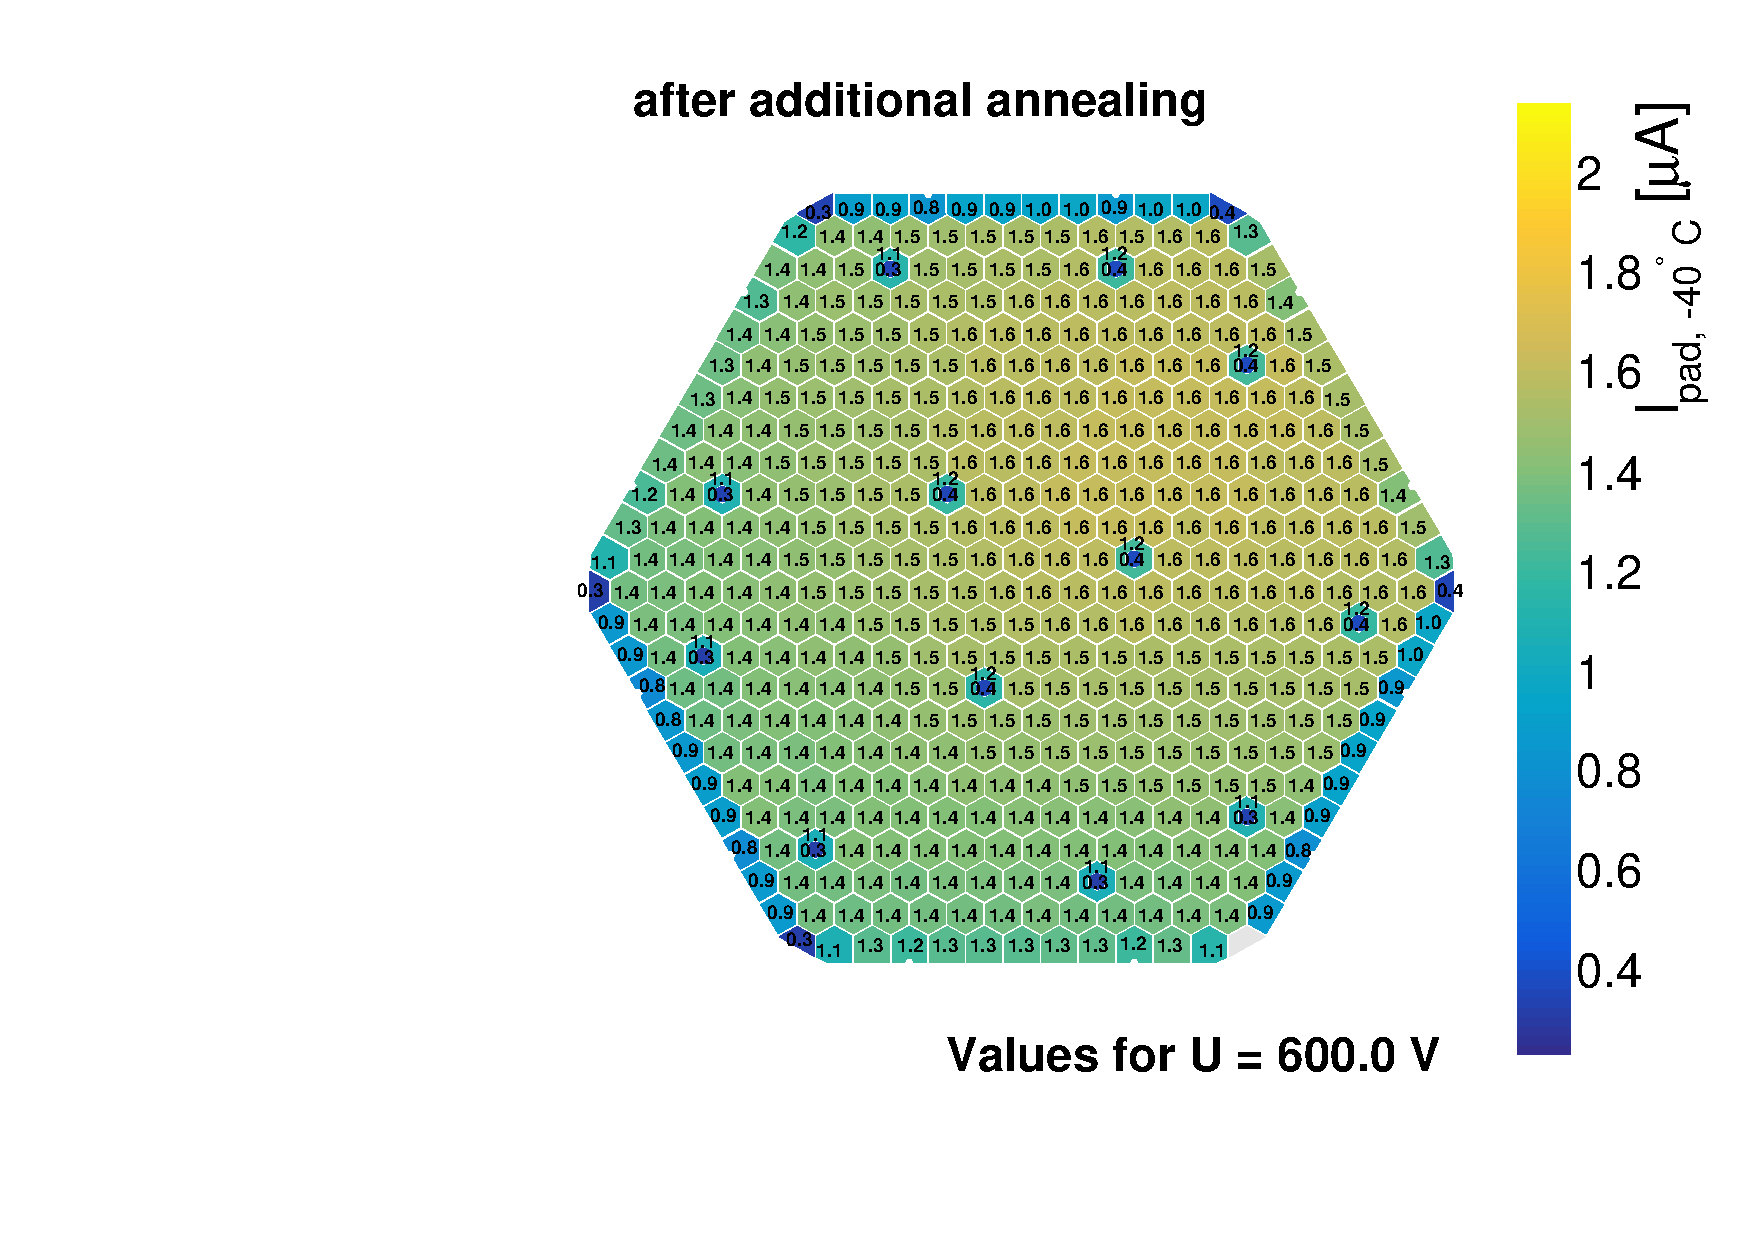
\includegraphics[width=0.999\textwidth]{plots/iv_hexplots/3009_annealed.pdf}
		\subcaption{
		}
		\label{plot:iv_hexplot_3009_annealed}
	\end{subfigure}
	\hfill
	\begin{subfigure}[b]{0.32\textwidth}
		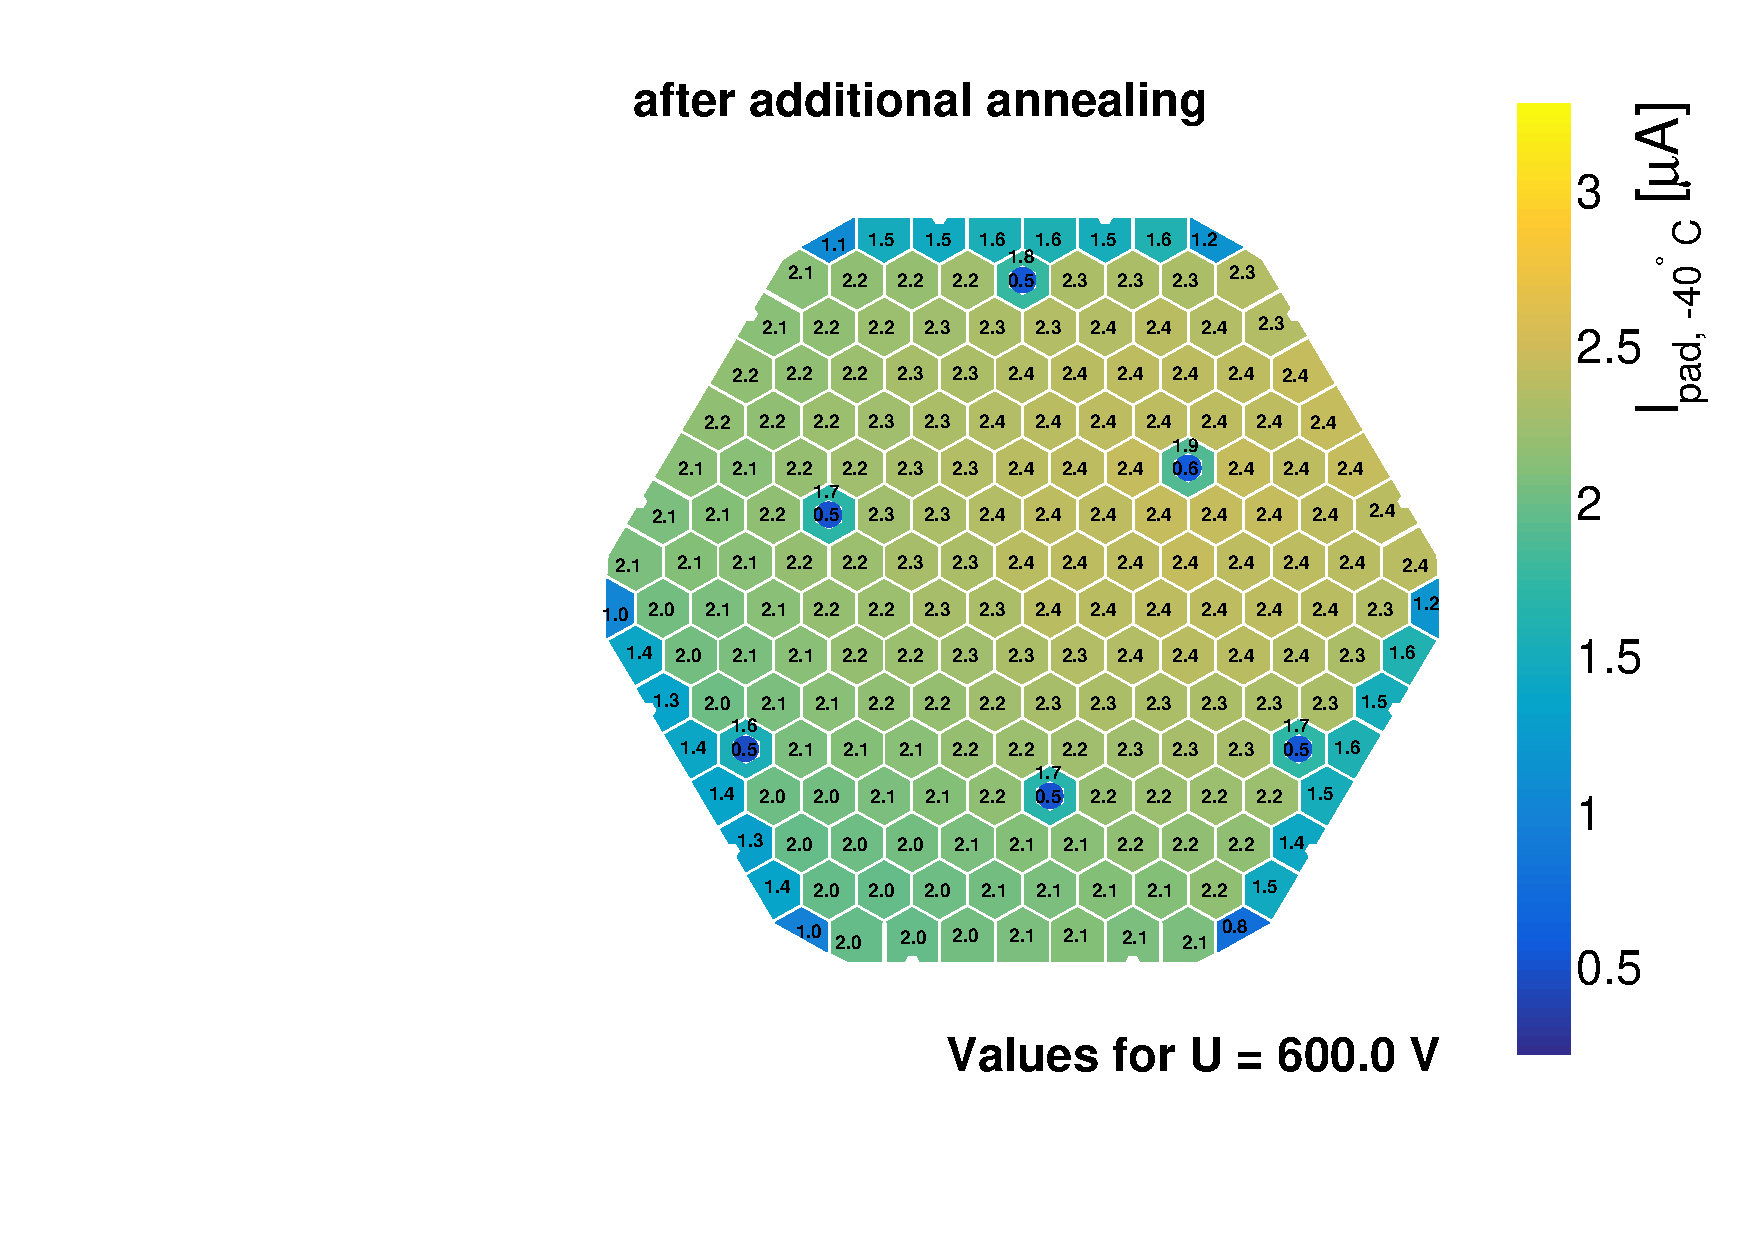
\includegraphics[width=0.999\textwidth]{plots/iv_hexplots/0541_04_annealed.pdf}
		\subcaption{
		}
		\label{plot:iv_hexplot_0541_04_annealed}
	\end{subfigure}
	\hfill	
	\begin{subfigure}[b]{0.32\textwidth}
		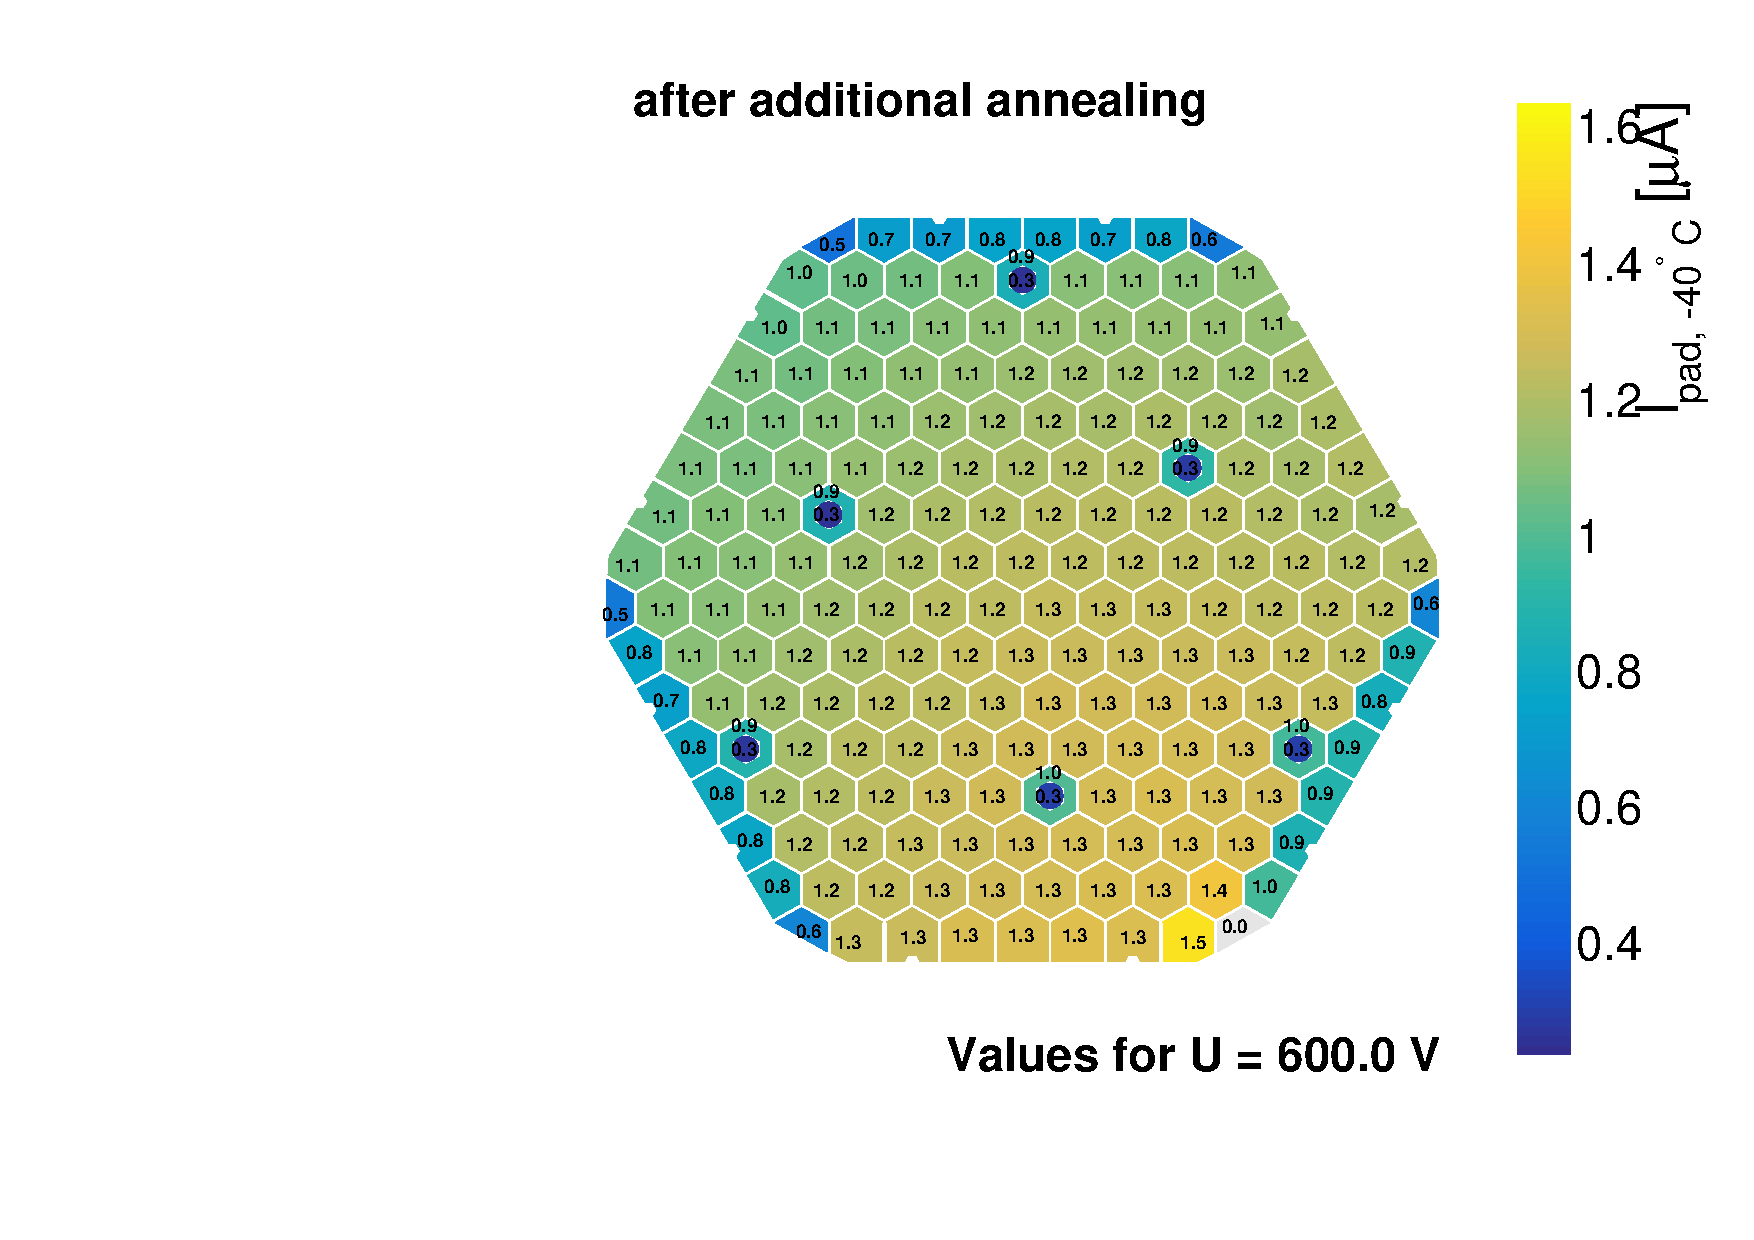
\includegraphics[width=0.999\textwidth]{plots/iv_hexplots/1013_annealed.pdf}
		\subcaption{
		}
		\label{plot:iv_hexplot_1013_annealed}
	\end{subfigure}    
	\caption{
		Per-pad leakage currents interpolated to an effective bias voltage of \SI{600}{\volt} for three representative sensors from different irradiation rounds before (a-c) and after additional annealing (d-f).
		Red- or white-colored edge pads correspond to well-understood measurement effects, e.g. insufficient contact between the pogo pins and the pads.
		}
	\label{plot:iv_hexplot}
\end{figure}


\subsection{Capacitance and Depletion Voltage}
\label{subsec:Udep}
The measured per-channel impedance is open-corrected by subtracting the impedance of the ARRAY system.
Subsequently, the sensor pad capacitance is computed assuming an underlying serial circuitry.
Due to the finite mobility of the sensor defects, the frequency at which the impedance is measured may, in principle, have sizeable impact on the hereby derived capacitance and on the depletion voltages for irradiated silicon pad sensors, cf. Ref.~\cite{Li1991}.
The impedance measurement for the results presented in this section was conducted at an LCR-frequency ($f_\text{LCR}$) of \SI{2}{\kilo\hertz}.
Experimental follow-up studies indicate a negligible impact of \SI{2}{\percent} on the asymptotic capacitance and a \SI{10}{\percent} reduction of the depletion voltage when decreasing $f_\text{LCR}$ to \SI{500}{\hertz}.
This dependence on $f_\text{LCR}$ has no practical implications on the following discussion.
The depletion voltage for each pad is assessed from the saturation of its squared reciprocal capacitance ($C^{-2}$) of a pad with respect to the effective bias voltage ($V$). 
It is defined as the intersection of a straight-line fitted to the rising part of the $C^{-2}$ vs. $V$ curve with a line fitted to its plateau.
Prior to additional annealing, such a plateau could not always be reached within the tested bias voltage range, see for example the black line in \ref{plot:annealing_CV}. 
After additional annealing to \SI{80}{\min} at \SI{60}{\celsius}, the estimated depletion voltage has been reduced by about a third with respect to the case without annealing, cf.~\ref{plot:annealing_Vdep}.
Only results from sensors after additional annealing are discussed in the following. 
\begin{figure}
	\captionsetup[subfigure]{aboveskip=-1pt,belowskip=-1pt}
	\centering

	\begin{subfigure}[b]{0.49\textwidth}
		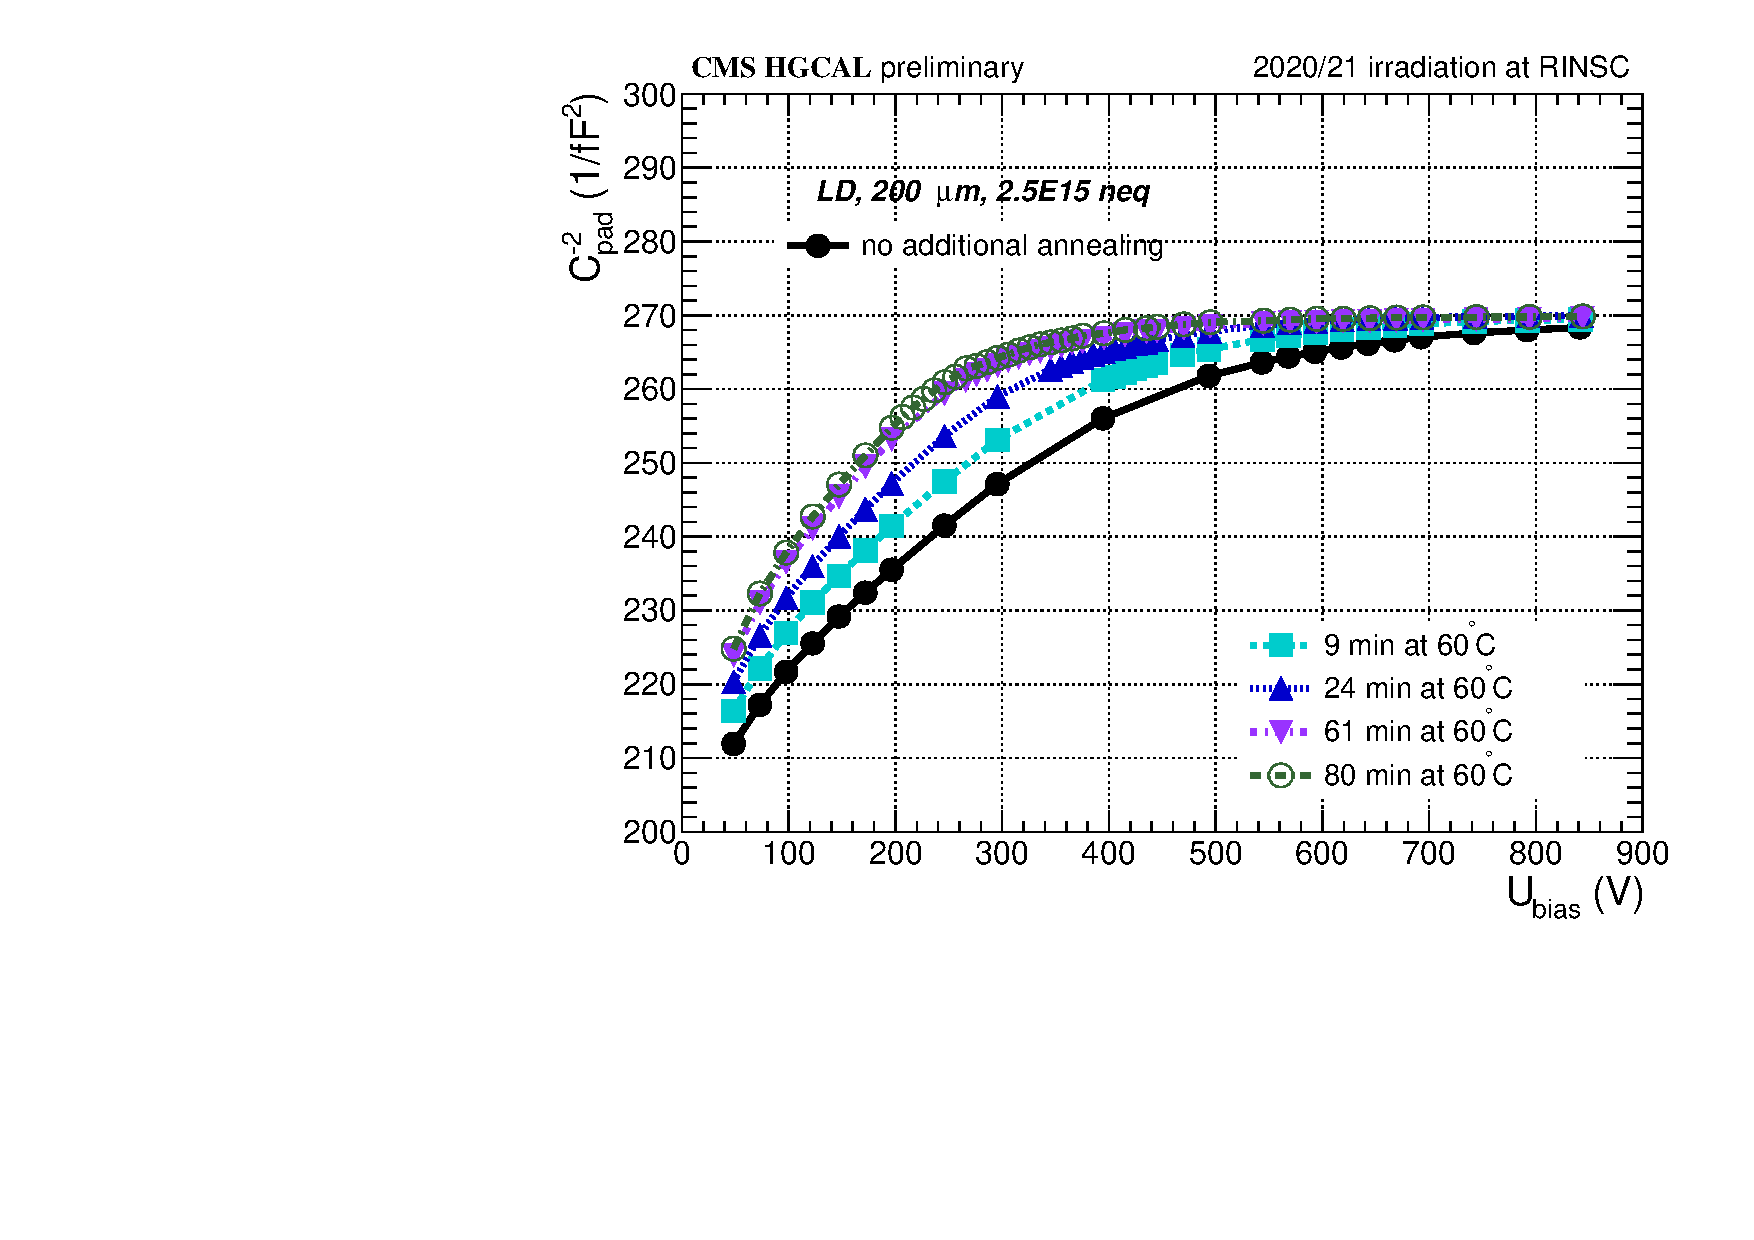
\includegraphics[width=0.999\textwidth]{plots/annealing_Vdep/annealing_CV_ch24.pdf}
		\subcaption{
		}
        \label{plot:annealing_CV}
	\end{subfigure}
    \hfill
    \begin{subfigure}[b]{0.49\textwidth}
		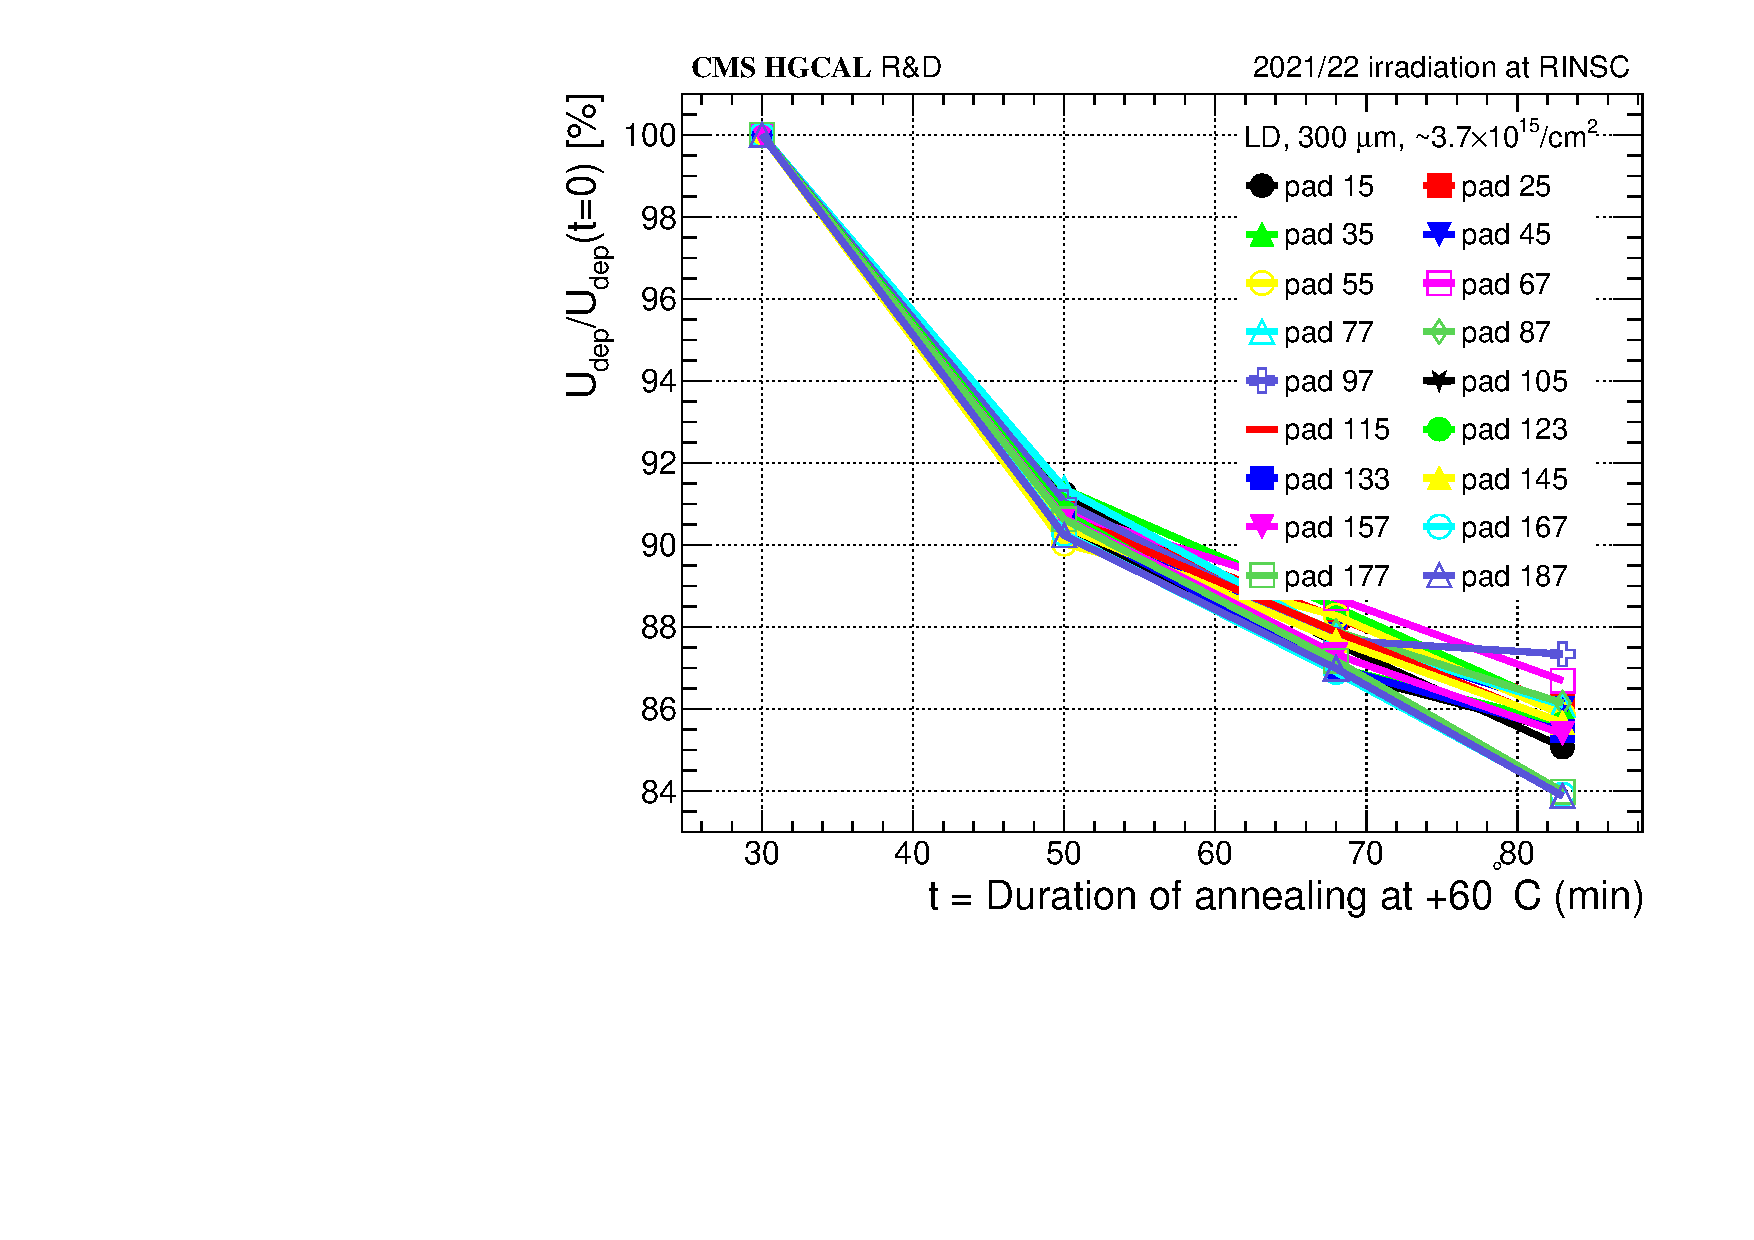
\includegraphics[width=0.999\textwidth]{plots/annealing_Vdep/annealing_Vdep.pdf}
		\subcaption{
		}		
        \label{plot:annealing_Vdep}
	\end{subfigure}
	\caption{
        (a) Reciprocal-squared capacitance ($C^{-2}_\text{pad}$) as a function the bias voltage of a representative full hexagonal pad for different annealing durations for a \SI{200}{\micro\metre} low-density prototype sensor irradiated to approximately 2.4$\cdot 10^{15}~\neqcm$.   
		(b) Relative decrease of the depletion voltage estimate ($U_\text{dep}$) as a function of the additional annealing time at \SI{60}{\celsius} for a subset of full pads.
	}
\end{figure}
\begin{figure}
	\captionsetup[subfigure]{aboveskip=-1pt,belowskip=-1pt}
	\centering
	\begin{subfigure}[b]{0.49\textwidth}
		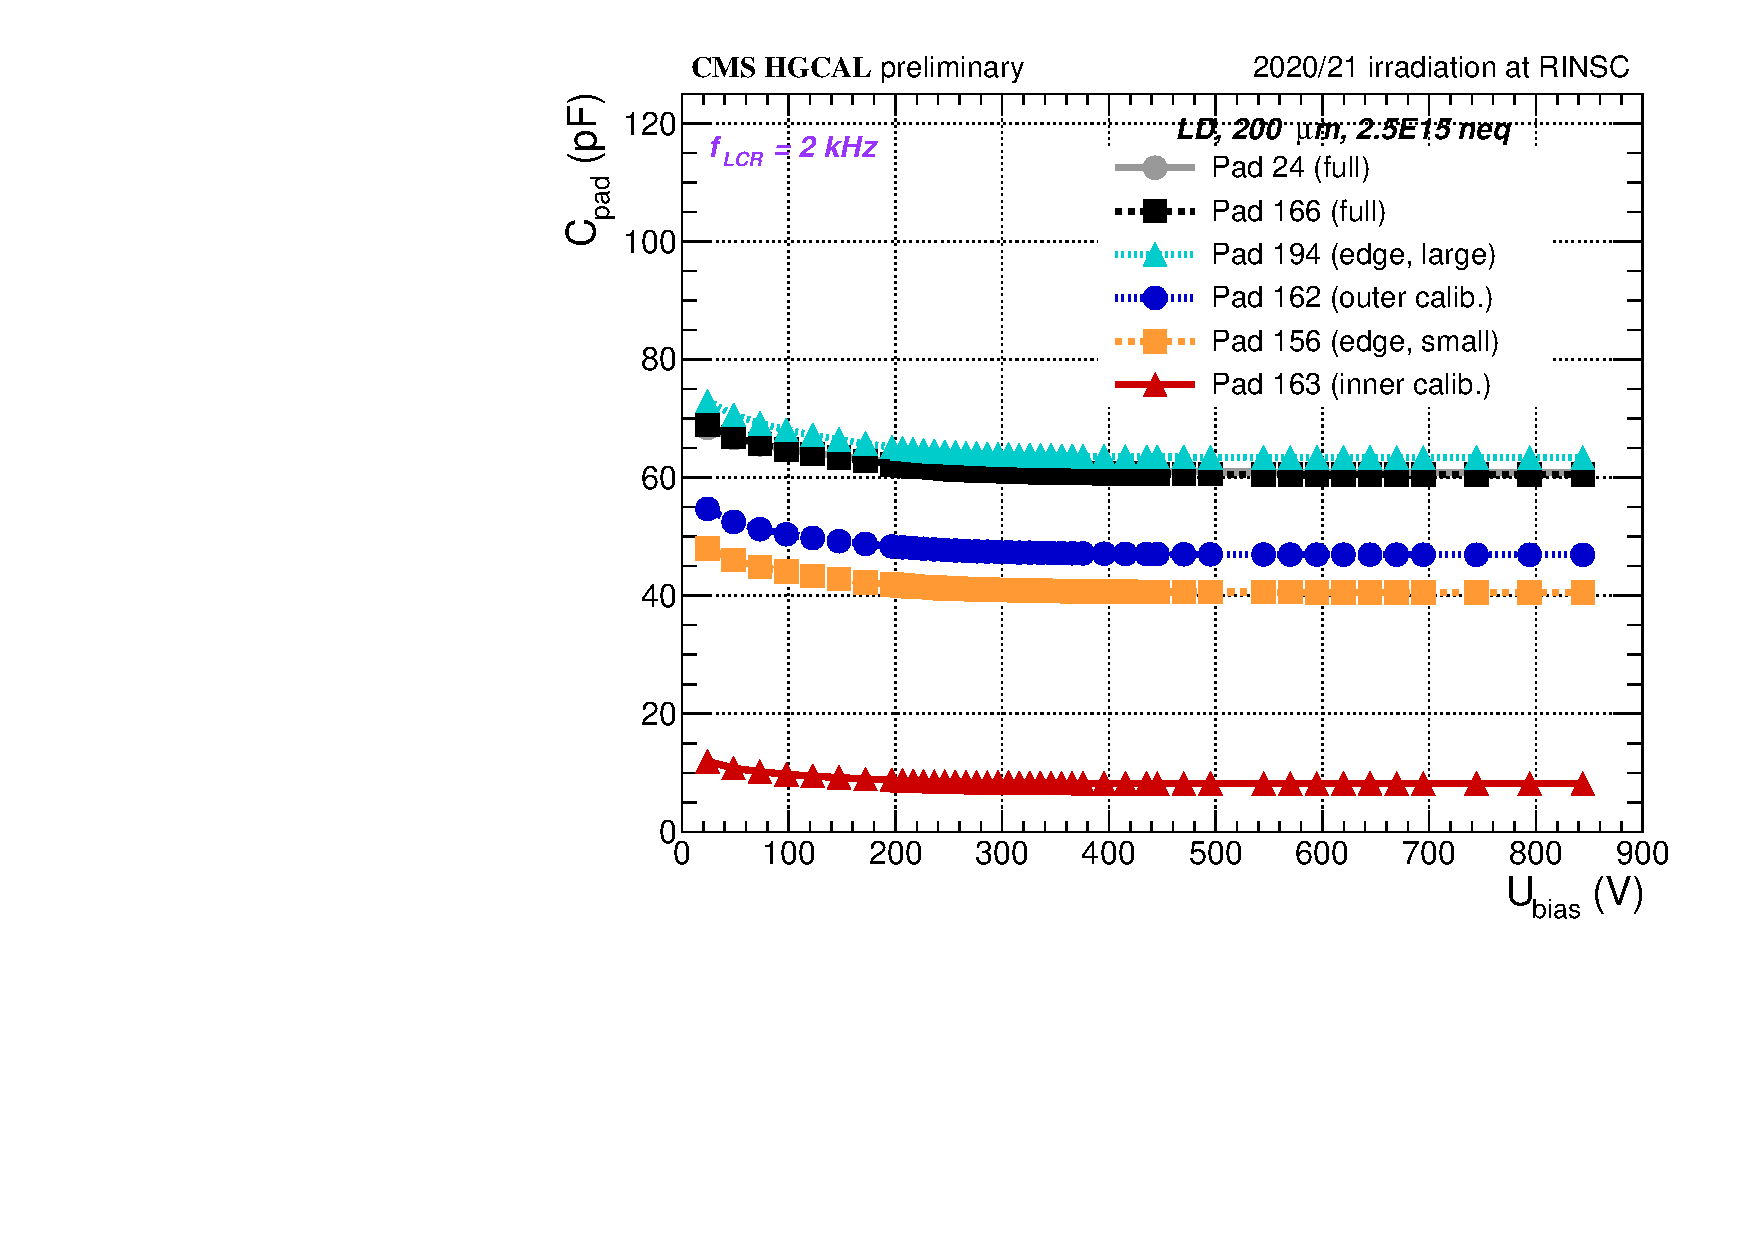
\includegraphics[width=0.999\textwidth]{plots/channel_cv/channel_CV_sensors_channels.pdf}
		\subcaption{
		}
		\label{plot:pad_CV_channels}
	\end{subfigure}
	\hfill
	\begin{subfigure}[b]{0.49\textwidth}
		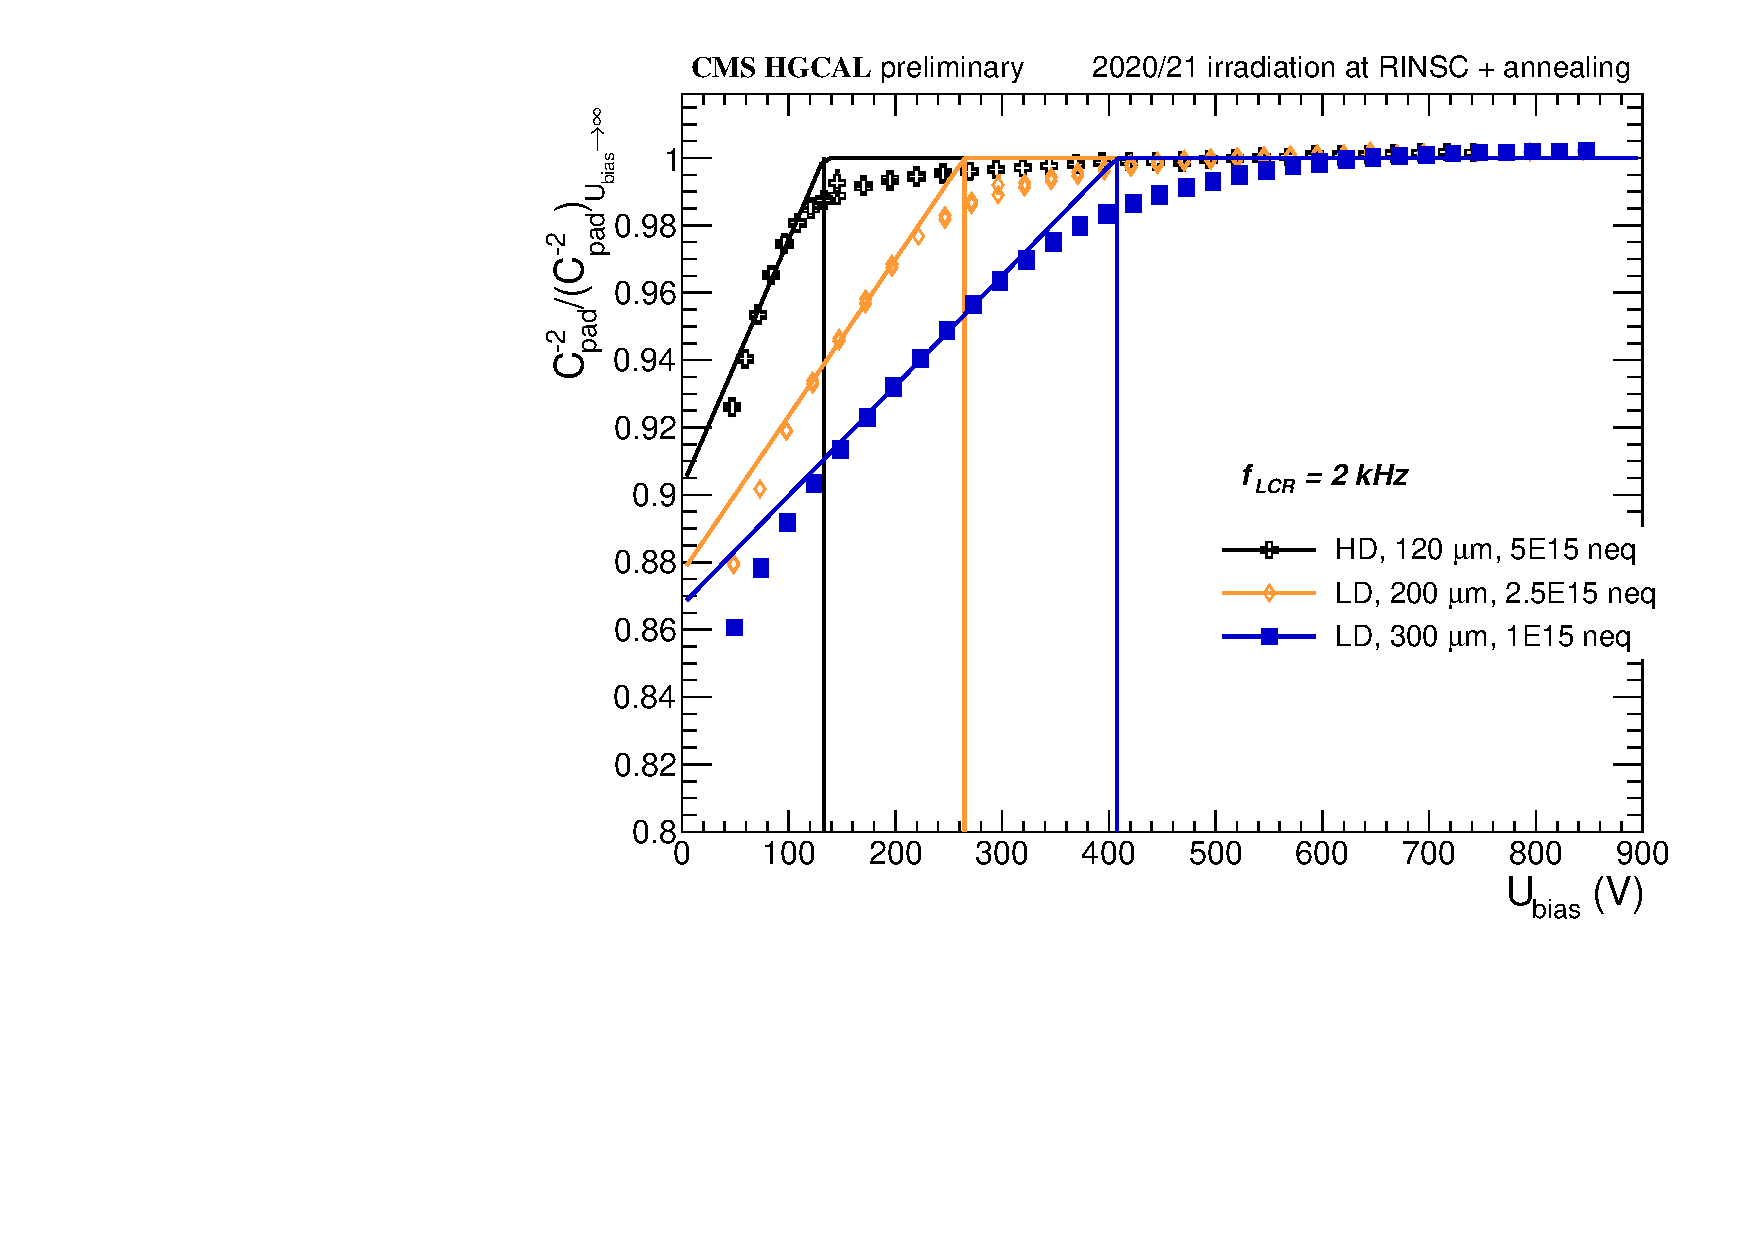
\includegraphics[width=0.999\textwidth]{plots/channel_cv/channel_invCV_sensors_sensors.pdf}
		\subcaption{
		}
		\label{plot:pad_invCV_sensor}
	\end{subfigure}
	\caption{
		(a) Area-normalised capacitances as a function of the effective bias voltage for different pads with different geometries on one example low density sensor.
		(b) Normalised squared-inverse capacitances as a function of the effective bias voltage for estimating the sensor depletion voltage for one central pad on three example sensors from different irradiation rounds.
		%The frequency of the Keysight E4980A LCR meter in these measurements was set to \SI{2}{\kilo\hertz}.
	}
\end{figure}
\begin{figure}
	\captionsetup[subfigure]{aboveskip=-1pt,belowskip=-1pt}
	\centering
	\begin{subfigure}[b]{0.49\textwidth}
		\centering
		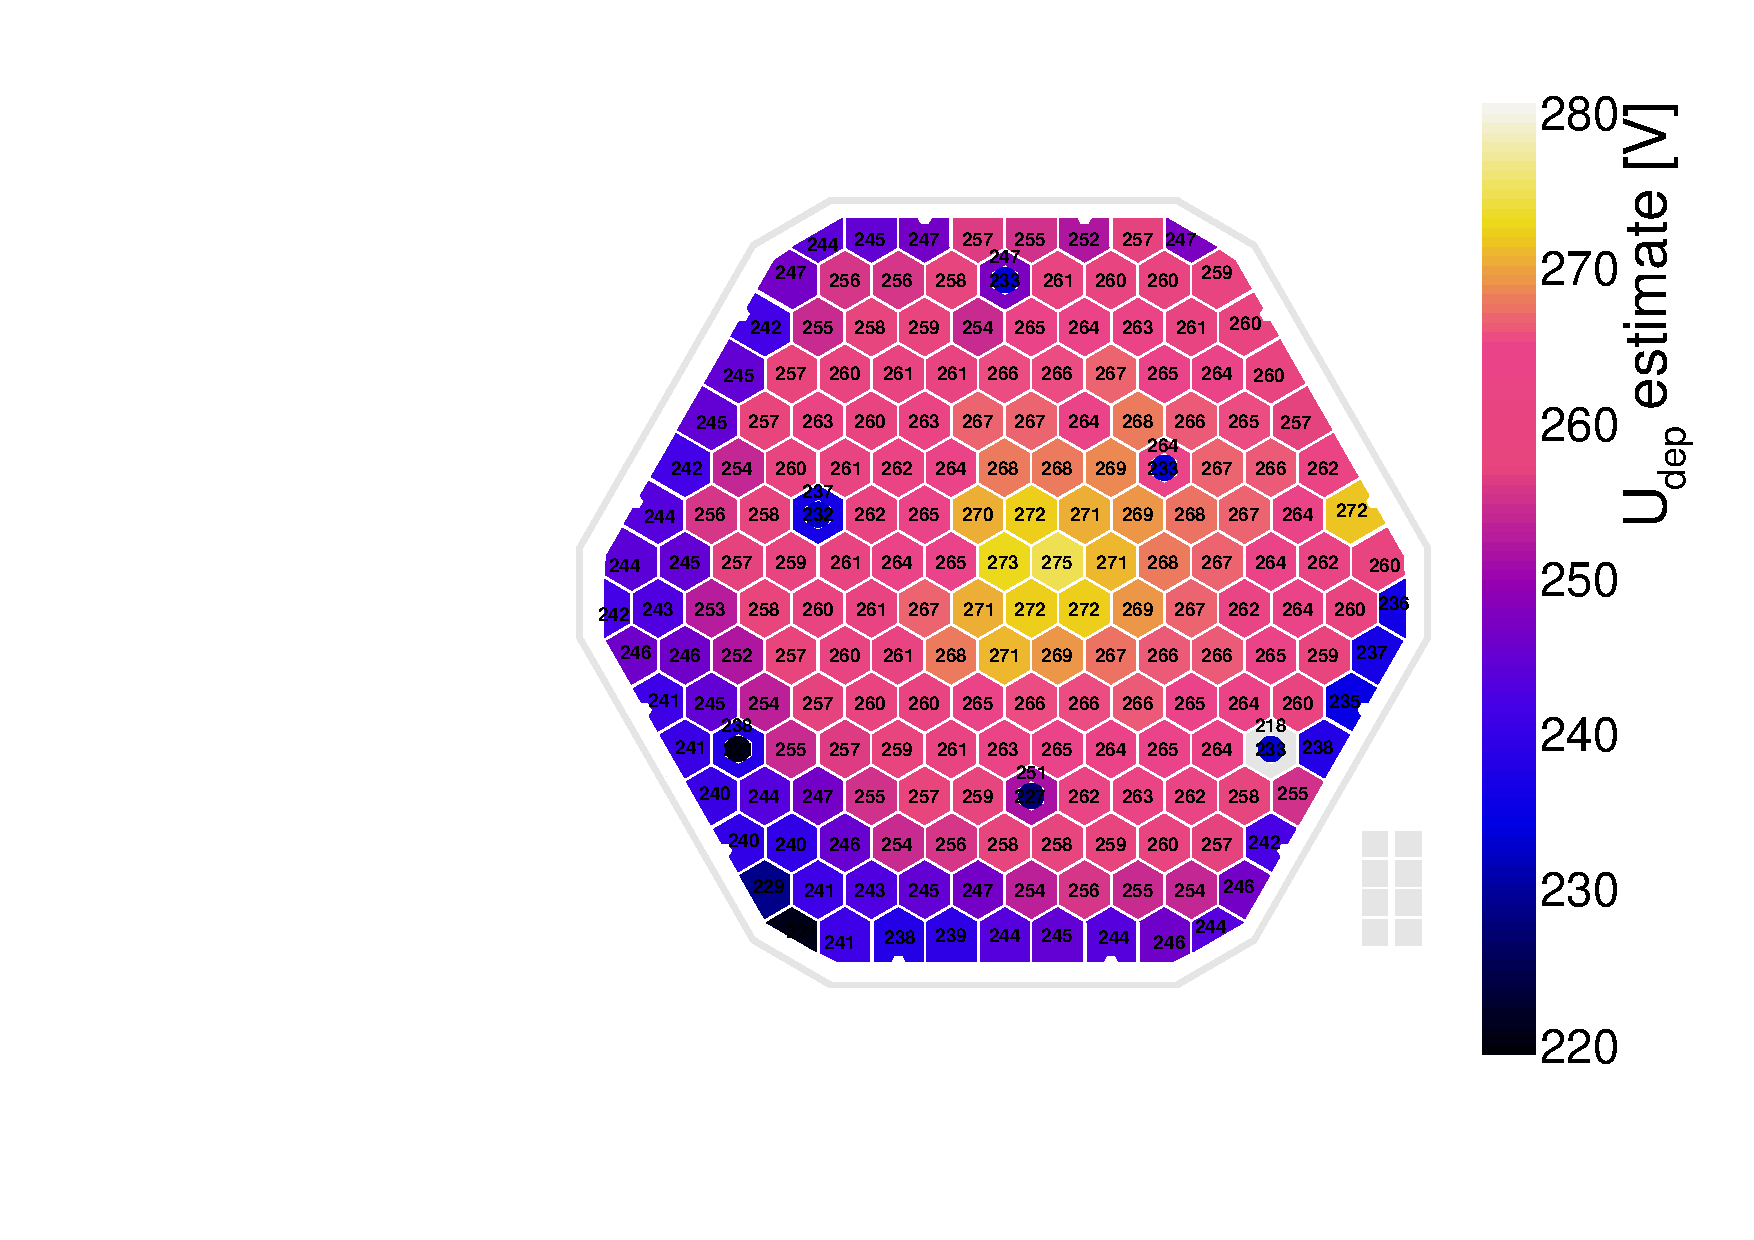
\includegraphics[width=0.99\textwidth]{plots/Vdep_hexplots/0541_04.pdf}
		\subcaption{
			}
			\label{plot:Vdep_hexplot_0541_04}
	\end{subfigure}
	\hfill
	\begin{subfigure}[b]{0.49\textwidth}
		\centering
		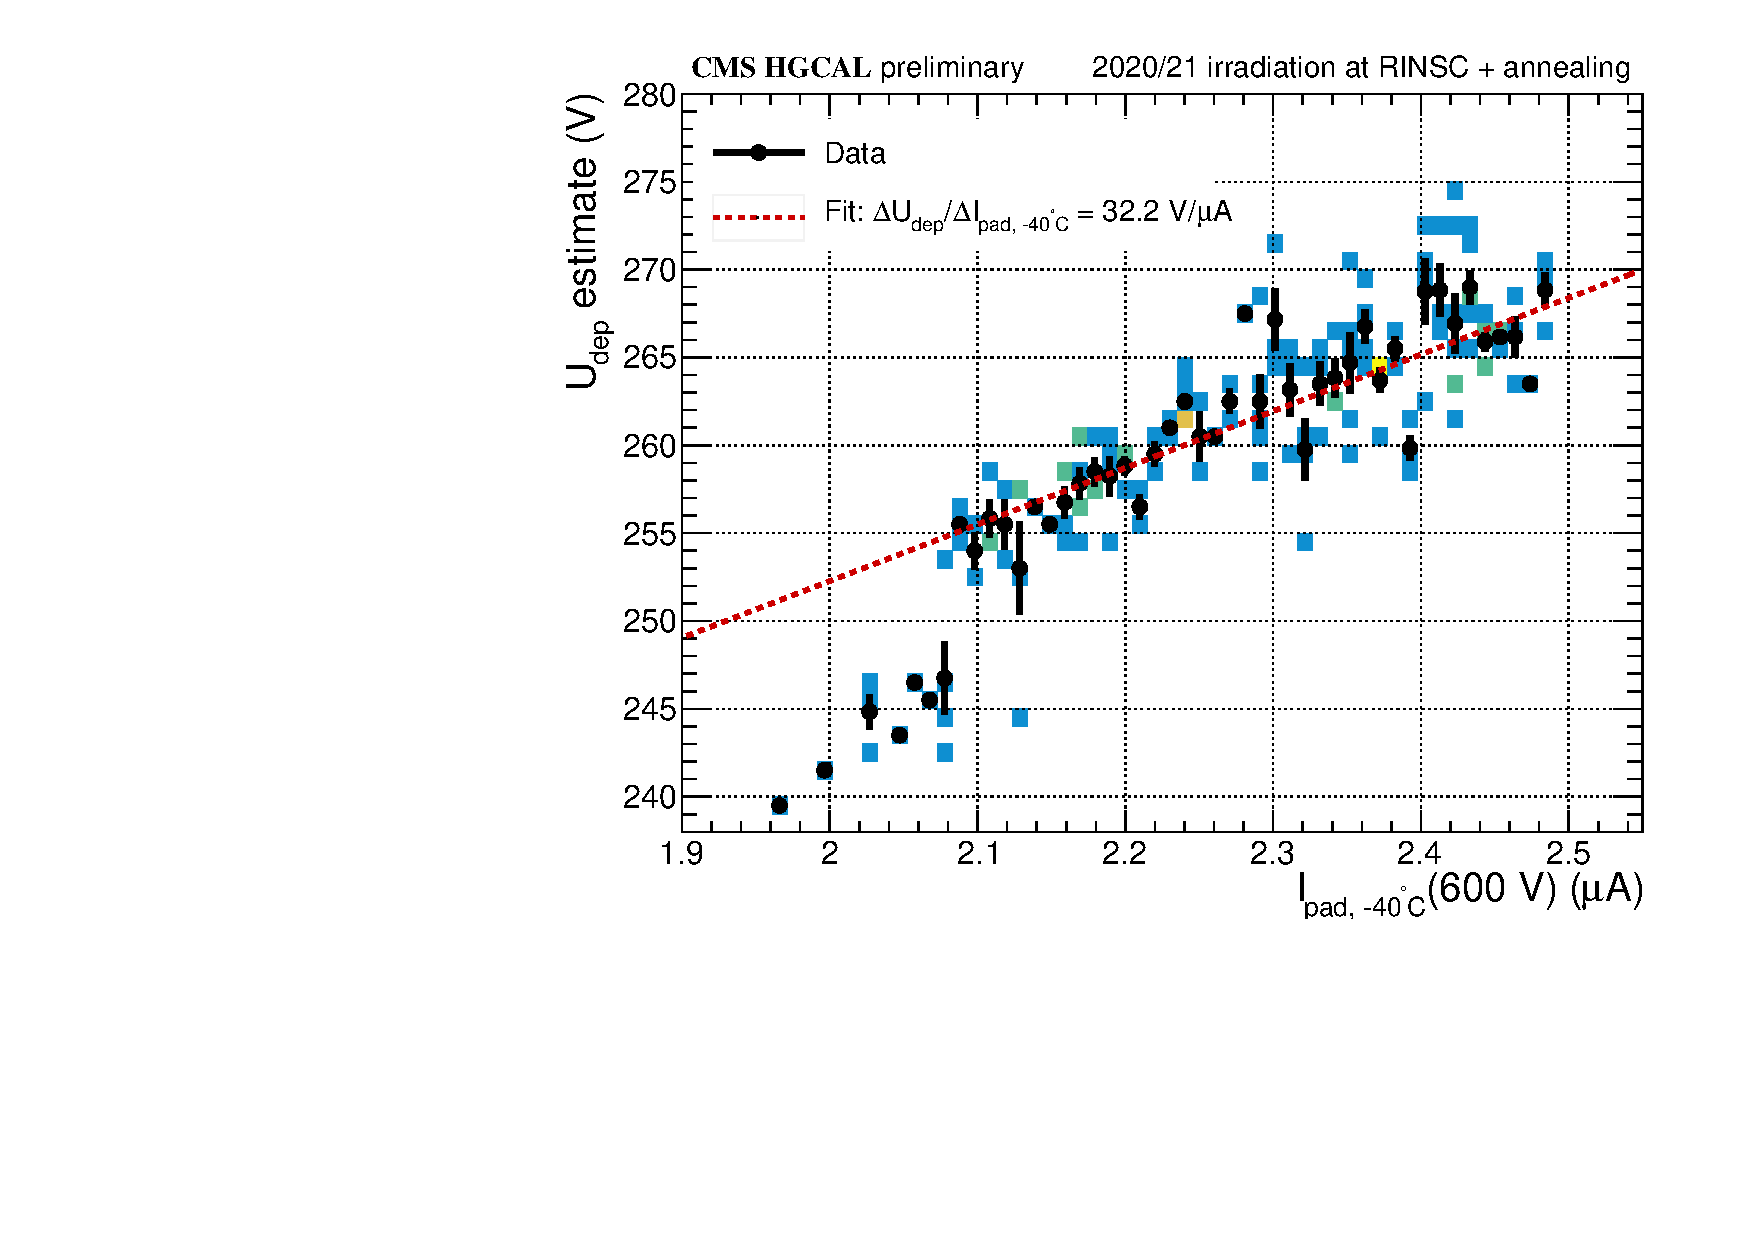
\includegraphics[width=0.999\textwidth]{plots/Vdep_vs_fluence/Vdep_vs_current_5414.pdf}
		\subcaption{
			}
			\label{plot:Vdep_vs_current_5414}
	\end{subfigure}
	\caption{
		(a) Per-pad depletion voltage estimates for a \SI{200}{\micron} LD example sensor irradiated to 1.9$\cdot 10^{15}~\neqcm$, and 
		(b) their correlation to the per-pad leakage current, used as proxy for the delivered fluence.
	}
\end{figure}
We find that the per-pad capacitance after irradiation scales reasonably well with the area of the pad, cf.~\ref{plot:pad_CV_channels}.
Deviations from this scaling amount to less than \SI{5}{\percent}.
The inter-pad capacitance has been in measured to be \SI{2}{\pico\farad}.
The deviation of the pad capacitance of up to \SI{5}{\percent} may hint at differing inter-pad capacitances between other pads geometries.
However, further investigation of this hypothesis is beyond the scope of this paper. 
\ref{plot:pad_invCV_sensor} illustrates that the estimated depletion voltages in this work scale primarily with the associated thickness of the depleted zone. 
The estimated per-pad depletion voltage across the sensor of a representative sensor is shown in~\ref{plot:Vdep_hexplot_0541_04}.
Those estimates exhibit positive correlation with the leakage currents, taken as proxy for the fluence, cf. \ref{plot:Vdep_vs_current_5414}.
In fact, the obtained correlation coefficient from this analysis is positive for all tested sensors where full depletion could be reached.
This circumstance can be understood as further evidence for the presence of a fluence profile inside the beam port during irradiation.

\subsection{Discussion}
\label{subsec:discussion}
The leakage currents measured from the neutron-irradiated silicon sensors in this work exhibit both qualitative and quantitative consistency with previous R$\&$D on irradiated silicon sensors, and in particular they are found to be independent on the tested silicon fabrication process (flatband voltage, p-stop).
Furthermore, unchanged end-capacitances and reduced depletion voltages after beneficial annealing are qualitatively consistent with previous R$\&$D.
The accurate determination of depletion voltages of irradiated silicon sensors is delicate and requires a thorough understanding of the underlying circuitry, in particular a dedicated choice of f$_\text{LCR}$ and of R$_\text{bias}$ on the switch card, and are biased by the choice of tested bias voltages.
Therefore and given that variations in those quantities are not a concern for the operation of HGCAL, we refrain from more quantitative statements on the depletion voltages and their variations between different sensor fabrication parameters at this point.\newline
Despite this limitation, our findings with the first prototypes of 8'' HGCAL silicon sensors are in full support of the radiation-hardness of their general design.
By implication, RINSC could be qualified as a valid facility for neutron irradiation of 8'' silicon sensors for the first time.
However, more accurate studies on the electrical sensor properties after neutron-irradiation would need to incorporate the systematic uncertainty on the effective annealing during irradiation, that is due to the temperature evolution and its potential lateral profile inside the reactor's beam port.
Similarly, an accurate assessment of the actual fluence at each pad would have to address the neutron flux profile, for whose existence this work provides first evidence.
\section{Conclusion}
\label{sec:conclusion}
\textcolor{red}{Todo.}
\acknowledgments
We thank the staff at the Rhode Island Nuclear Reactor for their support during the preparation and conduction of the neutron irradiations.
The former EP-LCD group at CERN has developed essential infrastructure, in particular the ARRAY system including the associated data acquisition software, and has co-financed the acquisition of the utilised cold-chuck probe station at CERN.
Without their input, this R$\&$D milestone towards the realisation of this novel calorimeter would not have been possible. 
We are thankful for the technical and administrative support at CERN and at other CMS institutes and thank the staffs for their contributions to the success of the CMS effort. 
We acknowledge the enduring support provided by the following funding agencies and laboratories: BMBWF and FWF (Austria); CERN; CAS, MoST, and NSFC (China); MSES and CSF (Croatia); CEA, CNRS/IN2P3 and P2IO LabEx (ANR- 10-LABX-0038) (France); SRNSF (Georgia); BMBF, DFG, and HGF (Germany); GSRT (Greece); DAE and DST (India); MES (Latvia); MOE and UM (Malaysia); MOS (Montenegro); PAEC (Pakistan); FCT (Portugal); JINR (Dubna); MON, RosAtom, RAS, RFBR, and NRC KI (Russia); MoST (Taipei); ThEP Center, IPST, STAR, and NSTDA (Thailand); TUBITAK and TENMAK (Turkey); STFC (United Kingdom); and DOE (USA).


\appendix
\section{Irradiation Rounds and Fluences}
\label{appendix:irrad_rounds}
See~\ref{table:irrads}.
\begin{table}[h]
	\centering
	\begin{tabular}{c|cccc}
		\textbf{Date} & \textbf{No. sensors} & \textbf{Duration} & \textbf{Fluence (\SI{1}{\mega\eV} neq/cm$^2$)} & \textbf{Reference} \\
		26 Aug 20 & 4 & \SI{13}{\minute} & 7.1E+14 & Si diodes \\
		%& 22 Sep 20 & 4 & \SI{38}{\minute} & E+14} & Si diodes \\
		20 Oct 20 & 4 & \SI{180}{\minute} & 110.0E+14 & Fe foils \\
		%21 Jan 21 & 4 & \SI{38}{\minute} & E+14 & Si diodes \\
		28 Jan 21 & 4 & \SI{38}{\minute} & 23.5E+14 & Si diodes \\
		%4 Feb 21 & 4 & \SI{180}{\minute} & E+14 & Fe foils \\
		11 Feb 21 & 4 & \SI{38}{\minute} & 16.5E+14 & Si diodes \\
		11 March 21 & 4 & \SI{76}{\minute} & 50.0E+14 & Fe foils \\
		01 March 21 & 4 & \SI{23}{\minute} & 13.5E+14 & Si diodes \\
		15 April 21 & 4 & \SI{15}{\minute} & 8.2E+14 & Si diodes \\
		06 May 21 & 4 & \SI{38}{\minute} & 19.0E+14 & Si diodes \\
	\end{tabular}
	\caption{Irradiation duration and estimated integrated fluences for the neutron-irradiation at RINSC of HGCAL prototype silicon sensors discussed in this work.
	The uncertainty on the fluence estimates amounts to 20$~\%$.
	}
	\label{table:irrads}
\end{table}



\section{Temperature Uniformity of the Systems att C200-40 Cold Chuck}
\label{appendix:chuck_temp}
The leakage current in silicon devices is dependent on the temperature.
For the investigated sensors in this work, the current is mainly generated in the bulk for which the temperature ($T$) and current ($I$) are related by~\ref{eq:temp_scaling}~\cite{Chilingarov_2013}, where $E_\text{eff}=\SI{1.21}{\electronvolt}$ is the effective gab energy and $k_b$ denotes the Boltzmann constant.
\begin{equation}
    \frac{I}{T^2}\cdot \exp{\frac{E_\text{eff}}{2\cdot k_b \cdot T}}~\equiv~\text{const.}
    \label{eq:temp_scaling}
\end{equation}
The validity of this temperature scaling law applied for the HGCAL silicon pad sensors in the relevant temperature range has been verified and is illustrated in~\ref{plot:iv_tempscaling}.
\begin{figure}[h]
	\centering
	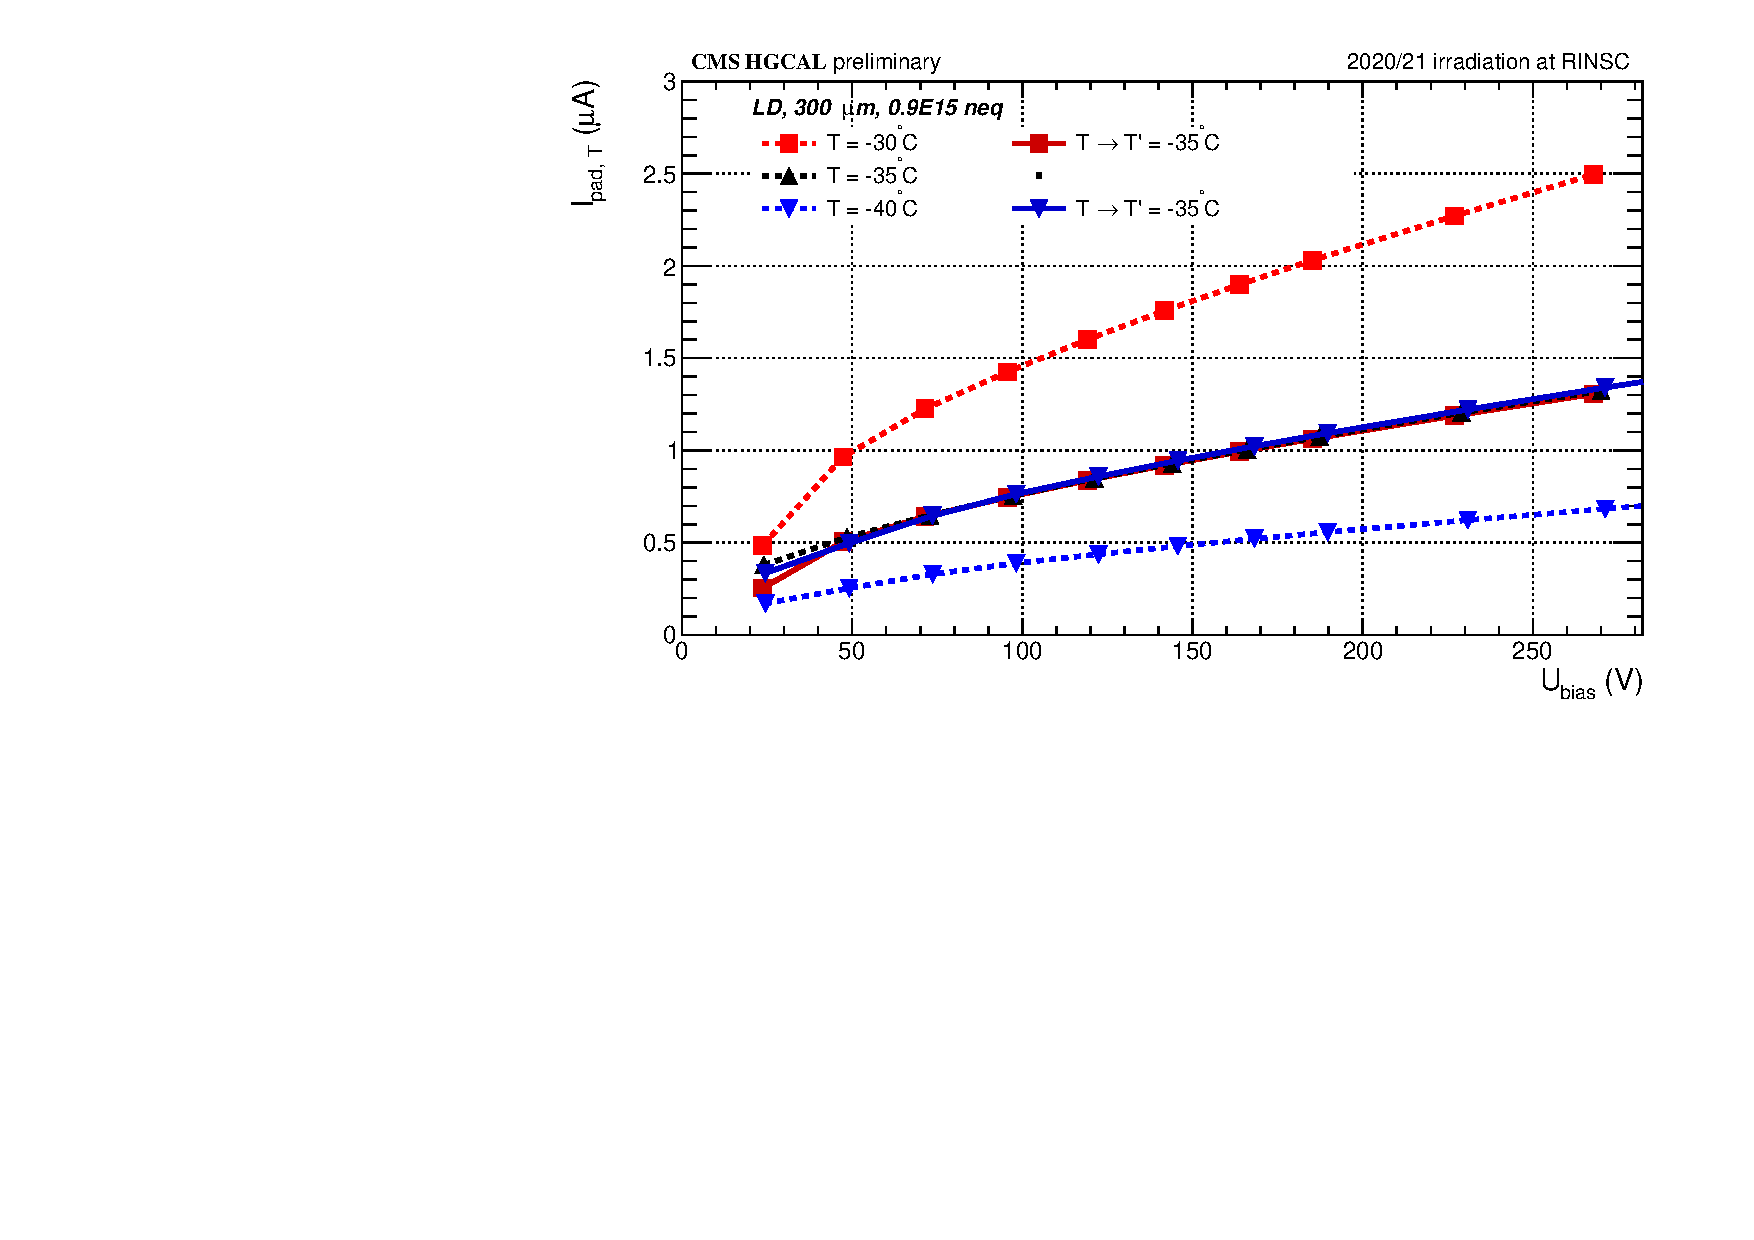
\includegraphics[width=0.69\textwidth]{plots/iv_temp_scaling/iv_overlay_ch24.pdf}
	\caption{
		Leakage currents as a function of the bias voltage for an example sensor measured at \SI{-40}{\celsius}, \SI{-35}{\celsius}, \SI{-30}{\celsius}, and scaled to \SI{-35}{\celsius} using$~$\ref{eq:temp_scaling}.
		}
	\label{plot:iv_tempscaling}
	\end{figure}
Notably, a change by \SI{1}{\celsius} impacts the current by more than 10$~\%$. 
Variations of the temperature across the chuck, and with it across the sensor, may mimic neutron fluence profiles as in~\ref{plot:iv_hexplot}. 
This, they should be identified and corrected for.\newline
In this work, the temperature non-uniformity of the cold chuck at CERN (C200-40 model produced by Systems att) could be estimated from leakage current data of neutron-irradiated sensors.
By comparing per-pad currents ($I_{i(j,k)}$) at a fixed bias voltage between symmetry locations $i$, $j$, $k$, temperature differences $\delta I_{i(j), k}$ can be calculated according to~\ref{eq:temp_diff}.
For this purpose, one of the neutron-irradiated low density sensor wafer was characterised three times at \SI{0}{\degree}, \SI{120}{\degree}, and \SI{240}{\degree} orientation.
The precision in repeating the sensor placement on the chuck can be neglected with respect to the size of the pads. 
\begin{equation}
    \frac{\delta I_{i(j),k}}{I_k} = \frac{\delta T_{i(j), k}}{T_k} \cdot \left(2 + \frac{E_\text{eff}}{2\cdot k_b \cdot T_k} \right)~,~~T_k \coloneqq T_\text{ref}
    \label{eq:temp_diff}
\end{equation}
\ref{plot:chucktemp_before} shows the hereby computed chuck temperature differences.
The determined variation is consistent with the $\pm\SI{0.5}{\celsius}$ non-uniformity as specified by the chuck producer.
Assuming a reference temperature of $T_\text{ref}\equiv\SI{-40}{\celsius}$, a two-dimensional gaussian parameterisation bound to $[\SI{-0.5}{\celsius}, \SI{0.5}{\celsius}]$ is fitted to reproduce the temperature differences $\delta I_{i(j),k}$.
The fit is performed with the tensorflow library (version 2.6.0) and the result is shown in~\ref{plot:chucktemp_correction}.
\begin{figure}
	\captionsetup[subfigure]{aboveskip=-1pt,belowskip=-1pt}
	\centering
	\begin{subfigure}[b]{0.32\textwidth}
		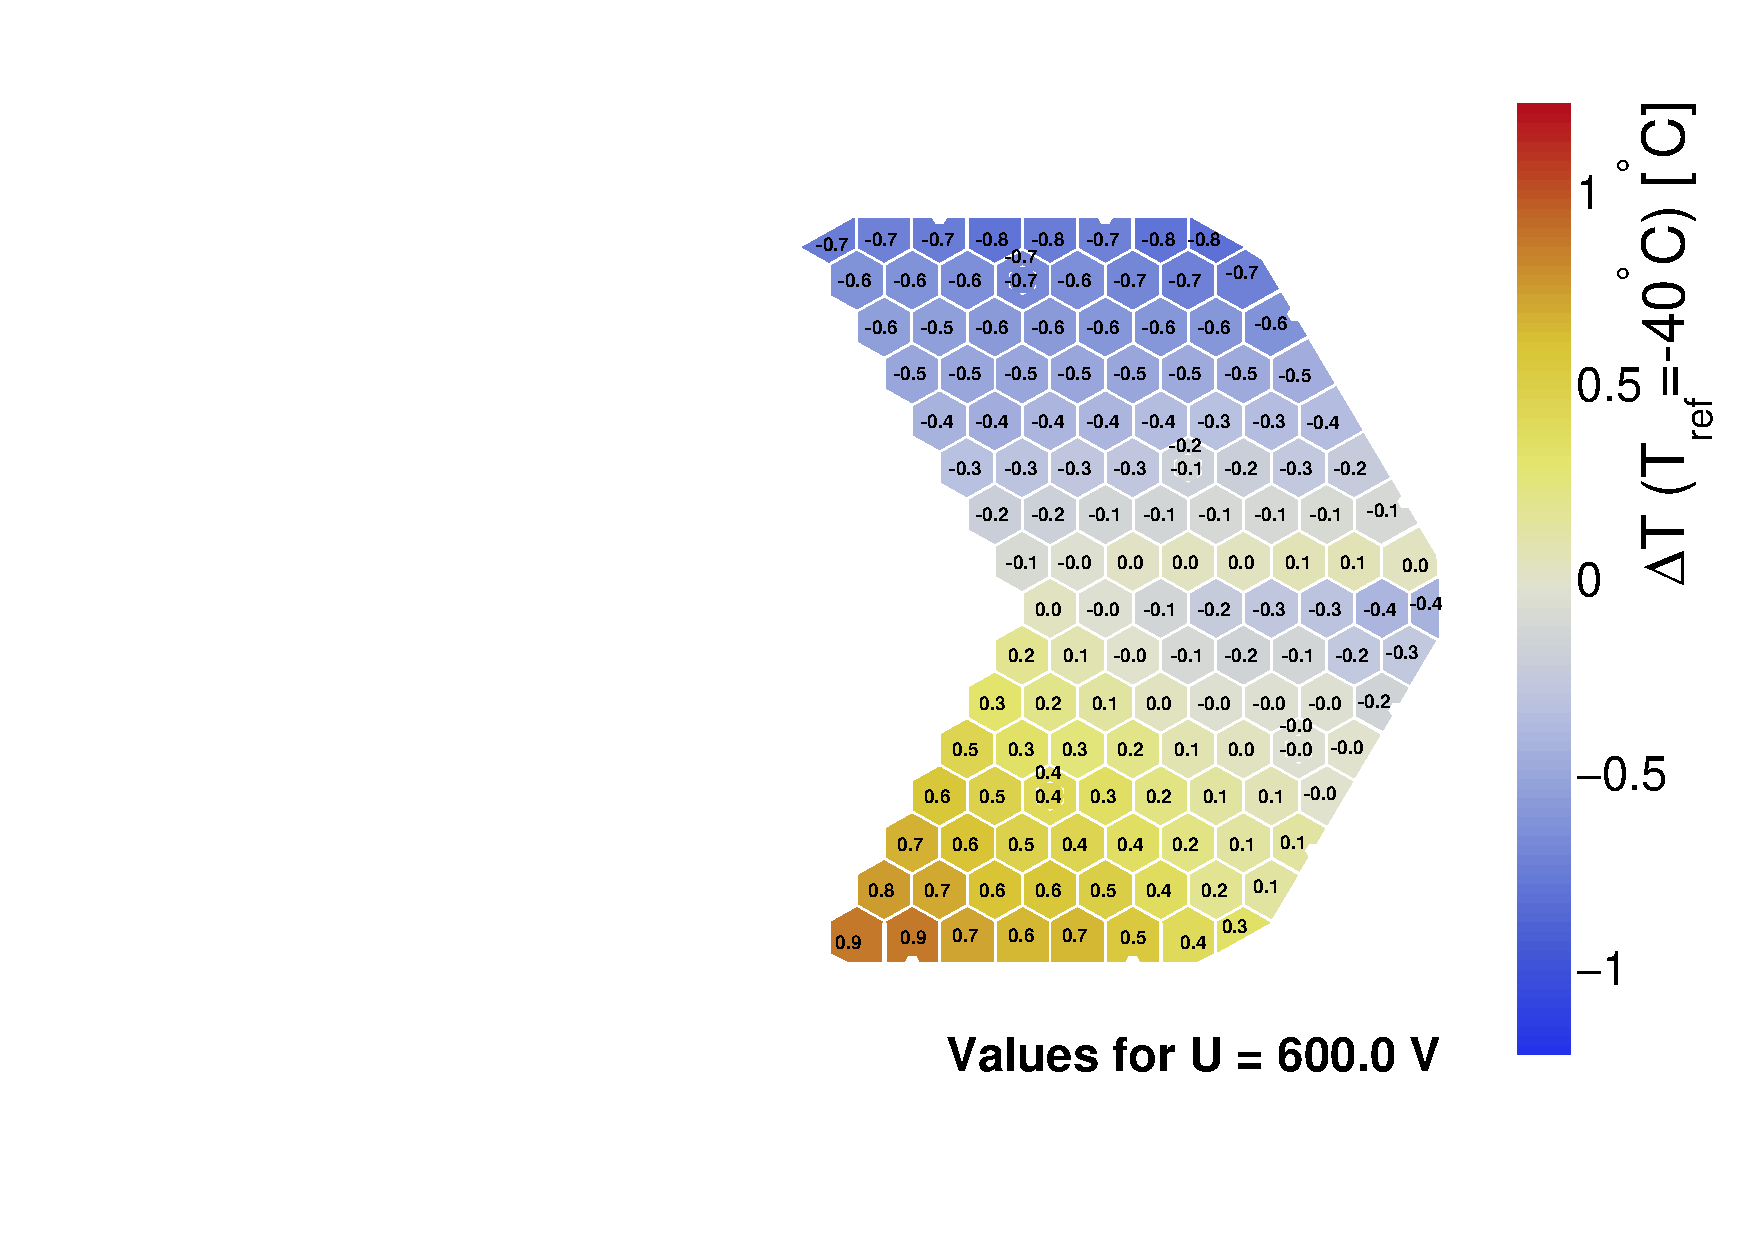
\includegraphics[width=0.999\textwidth]{plots/chuck_temp_correction/Spring2021_ALPS.pdf}
		\subcaption{
		}
		\label{plot:chucktemp_before}
	\end{subfigure}
	\hfill
	\begin{subfigure}[b]{0.32\textwidth}
		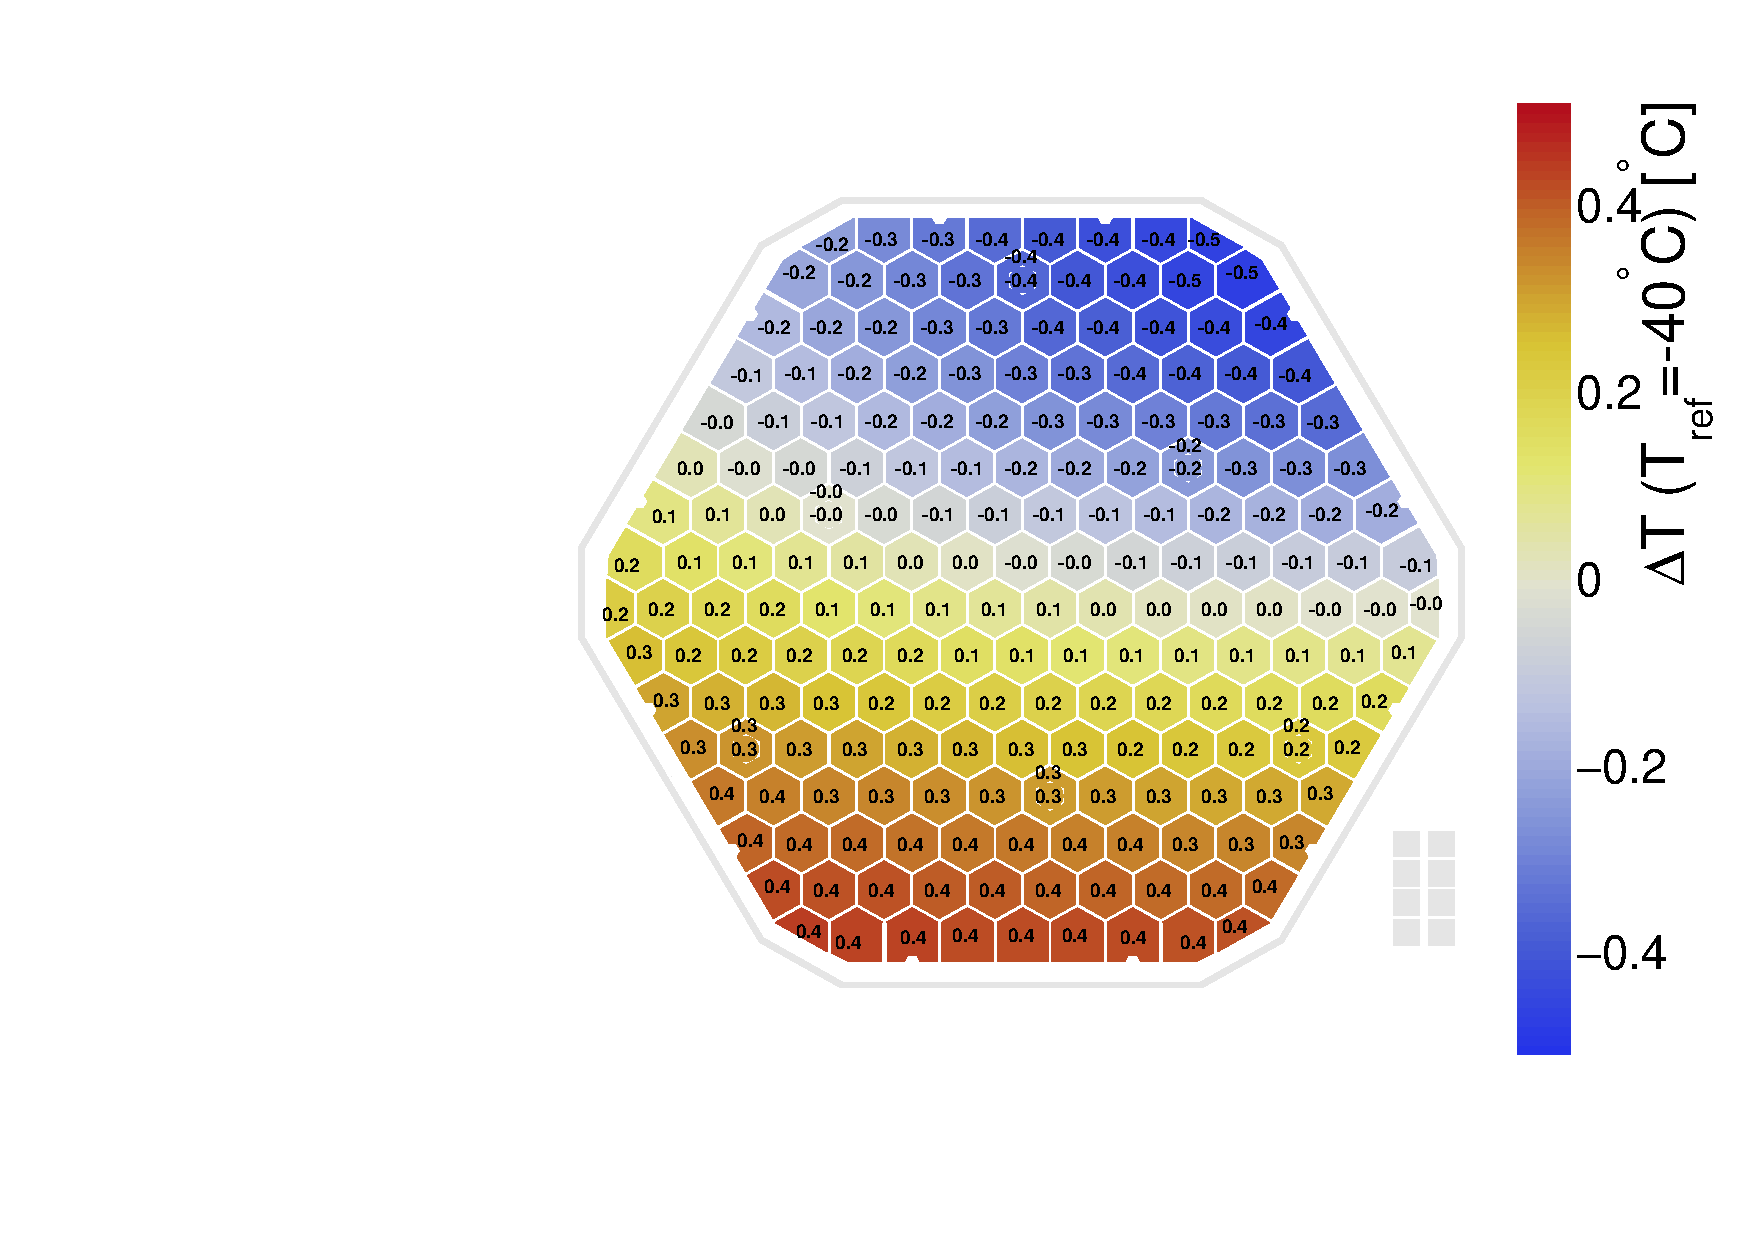
\includegraphics[width=0.999\textwidth]{plots/chuck_temp_correction/Spring2021_ALPS_deltaT.pdf}
		\subcaption{
		}
		\label{plot:chucktemp_correction}
	\end{subfigure}
	\hfill
	\begin{subfigure}[b]{0.32\textwidth}
		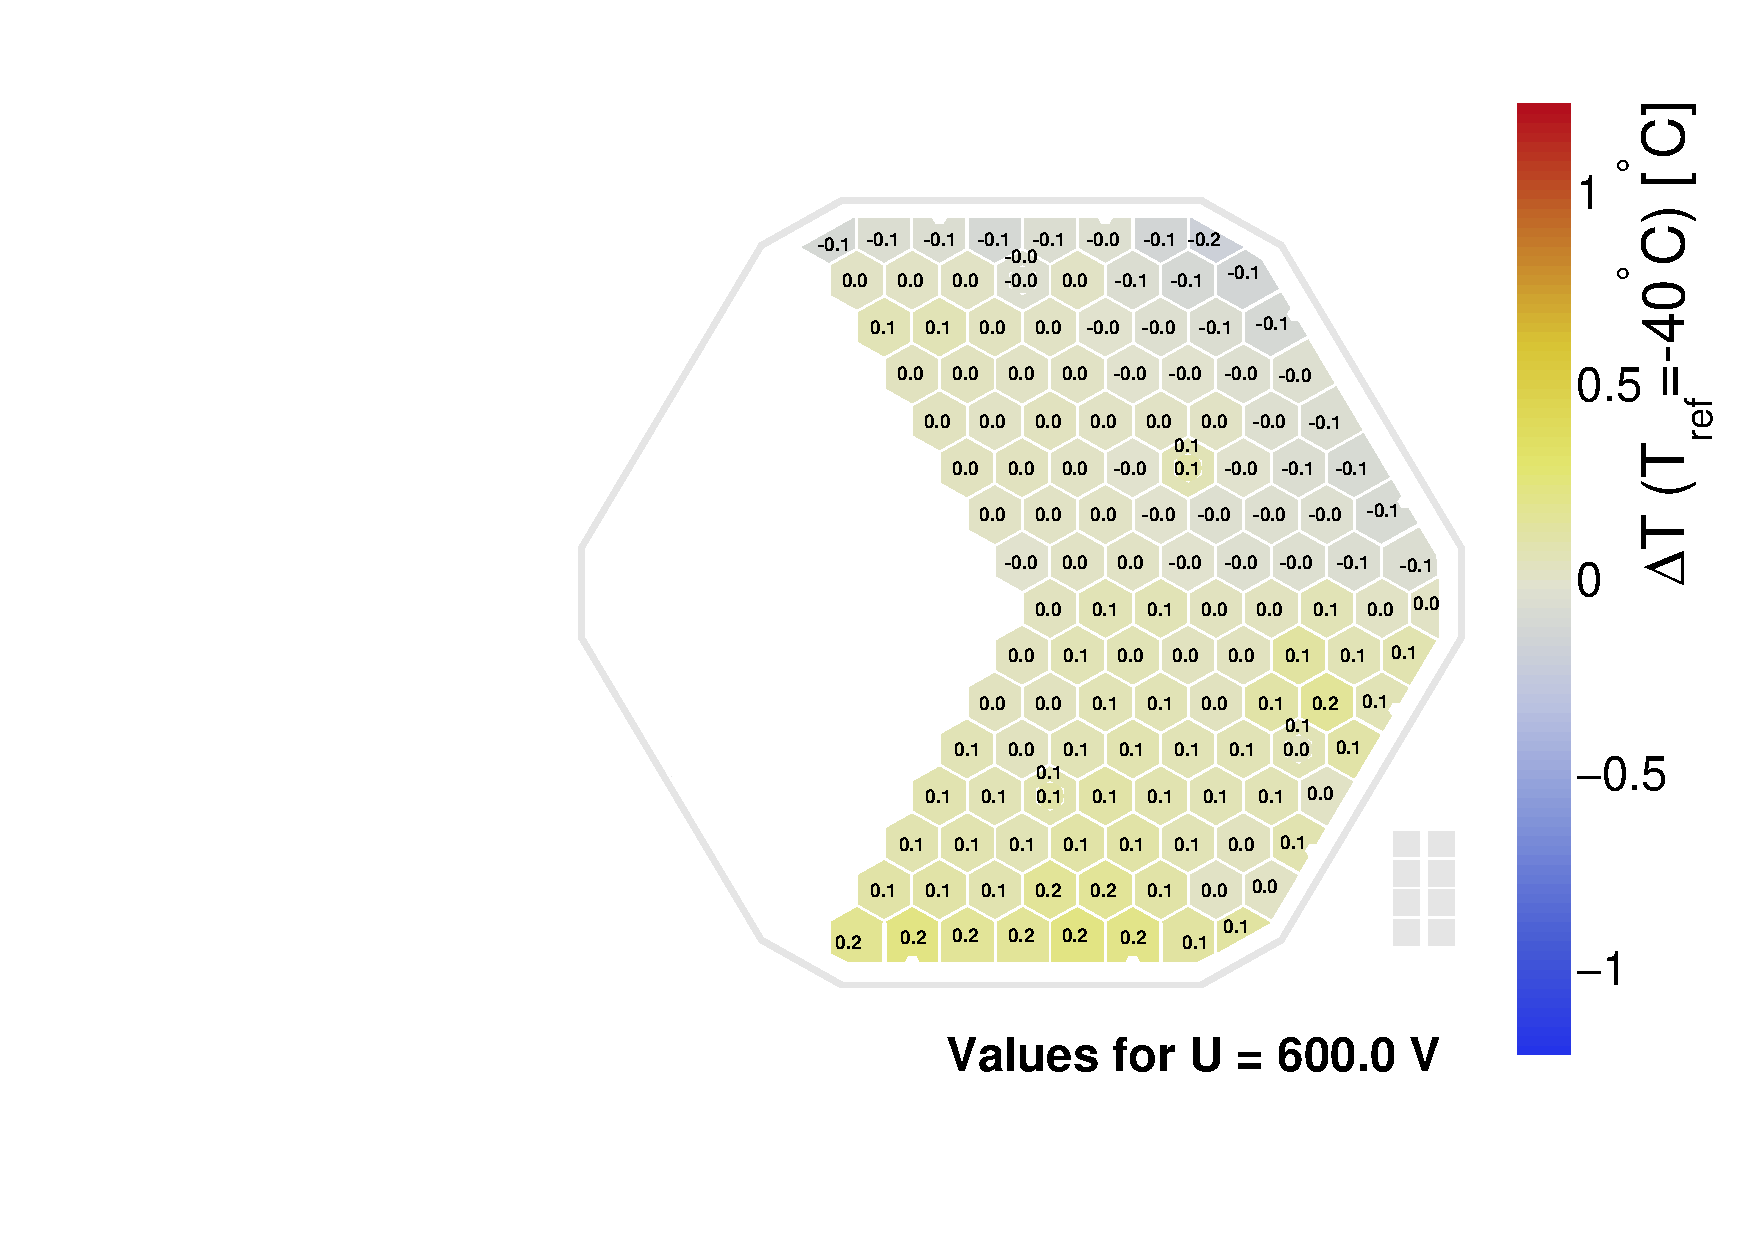
\includegraphics[width=0.999\textwidth]{plots/chuck_temp_correction/Spring2021_ALPS_chucktempcorrected.pdf}
		\subcaption{
		}
		\label{plot:chucktemp_after}
	\end{subfigure}
	\caption{
		(a) Temperature differences derived from per-pad leakage currents between symmetry locations of a representative neutron-irradiated HGCAL silicon sensors on the cold chuck at CERN.
		(b) Determined profile of temperature differences, modelled as a two-dimensional gaussian, across the sensor surface.
		(c) Closure check: Derived temperature differences after accordingly correcting the measured per-pad leakage currents.
	}
\end{figure}
The hereby constructed map of chuck temperature differences is input to correct the measured per-pad leakage currents using~\ref{eq:temp_scaling}.
As a closure check, the re-application of~\ref{eq:temp_diff} on the temperature-corrected dataset demonstrates the applicability of this particular chuck temperature model.


\bibliographystyle{unsrt}
\bibliography{bib/bib}

\end{document}
